\usepackage{amsmath}
\usepackage{adjustbox}
\usepackage[
backend=biber,
style=numeric, %TODO ask 
]{biblatex}
\addbibresource{mobius.bib}
\addbibresource{icp.bib}
\addbibresource{bibliography.bib}
\addbibresource{how-kinect-work.bib}
\addbibresource{linemod-origins.bib}
\addbibresource{primesense-patent.bib}
\addbibresource{stereo-vision-robot.bib}
\addbibresource{stereo-precision.bib}
\addbibresource{grasp-training.bib}
\addbibresource{bombarolo.bib}
\addbibresource{extinction.bib}
\addbibresource{pisa-softhand.bib}
\addbibresource{computervision.bib}

\newcommand{\vmiddle}[1]{\begin{tabular}{@{}c@{}} {#1} \end{tabular}}
\begin{document}
\english
\tableofcontents
\listoffigures
\listoftables
\chapter{Introduction}
Robotics has always been an appealing research field for many
application fields. Since the first industrial revolution, machinery
has been built in order to automate repetitive tasks which had been
completed by humans before that moment. This process brought the
entire humanity to change its way of life, bringing the main part of
society from an agricultural, artisanal system to a modern,
industrialized one. In general, this has been pointed out as one of
the biggest turns in the human history, which changed almost every
aspect of people's life; although many changes due to the automation
processes have been seen as catastrophic by some, such as
\cite{bombarolo} and \cite{extinction}, mainly because of the
increased gap between wealthy countries and poorest ones, it is
undeniable that the increase of material richness which has come as a natural
consequence of all of this is a great benefit for any person.

In the first century since industrial revolution, research on
automation has focused on applying new technological discoveries to
special-purpose machines; this has brought to automating tasks like
cloth washing, objects' manufacturing, and warehouses' management.

However, this approach has shown its drawbacks in recent times: having
a different machine for each single task, especially in case of
factory automation ones, pays a lot in terms of flexibility of the
machine itself, and this brings a much higher cost in the scenario,
which is going to be actually very common in the near future, in which
a factory wants to automate its whole structure. Also, recent
technological improvements have lowered a lot the need of
mechanics-based machinery, preferring solutions based on electronics
and complex software. This allowed a further push on automatic tasks'
completion by reducing a lot the cost of machinery (expect for
non-recurring engineering costs) due to limited material cost, which
are the most important to optimize in a world based on
mass-production. Thus, research on automation has moved to find a
solution for completing general tasks, in order to obtain, in the far
future, a robotic product which will have the ability to substitute
almost completely humans in labour.

The main research projects operating with this goal have, for obvious
reasons, focused their efforts on the study of \emph{humanoid
  robotics}, as the human body is, by an engineering point of view,
one of the most optimized, general-purpose machines in existence,
being capable of directly fulfilling extremely complex tasks, except for the
ones needing extreme precision or strength to complete. From this point of view, a
robot able to compare with the human brain in terms of decision capabilities
would make the general automation task totally completed, bringing to
the complexity of human intelligence the added value of virtually
infinite working strength and precision, due to its ad-hoc mechanical
and electronic components.

One of the main application fields in which human-like robotic devices
have always had their space is the one of objects' manipulation. In
fact, since the beginning many automatisation tasks involving
nontrivial handling of items, notably pick-and-place into
manufacturing pipelines, have been solved by usage of human-like
robotic arms, which for this reason gained their own industrial sector
since the early '70s, with the birth of companies like the Italian COMAU,
producing industrial automation solutions from the start, and the
expansion of others like the German KUKA, which moved its commercial
focus from the production of goods for manual use (wielding equipment,
communal vehicles) to the development of automated industrial robots,
which lead to the production of the first 6-DOF electric robot, named
\emph{FAMULUS}, in 1973.\footnote{http://www.kuka-robotics.com/usa/en/company/group/milestones/1973.htm}

Picking objects has thus always been a fundamental task for all of this
scenarios, and can nowadays be considered fully solved in most
cases. However, this are again all special-purpose solutions: most of
these solution are built for situations in which the pose of the
objects which will have to be manipulated is known a-priori, as they
are often coming from a preceding section of a production pipeline,
and the set of movement which the object will have to do is fixed
too. Thus, an ad-hoc solution can be studied and built, and the robot
can be thought, built and programmed to fulfil robustly its unique
task. The more general manipulation scenario, in which a robot is able
to be instructed at runtime to which object to take, how to manipulate
it, and where to find it, is far beyond the current state of the art
in robotics. Neverthless, research is growing more and more
quickly on this topic; it would, in fact, lead to virtually infinite
new opportunities for a lot of fields. One of the most important use
cases for this include
the relatively recent growth of e-commerce platforms, such at the 
most known company of this sector, \emph{Amazon.com, Inc.}, or the
online retail platform \emph{Overstock.com, Inc.}, which has become
famous as the first major e-commerce platform to accept Bitcoin as a
valid currency. Automated object manipulation is, anyway, absolutely
not limited to big companies' automation systems: another utility case
is the use of mobile, robotic platforms, equipped with robotic arms,
for domotic and household tasks, either to bring further ease in
domestic work, or to help diseased people, especially if with motion
or mental impairment. In this case, a human-like robotic arm, or a
complete humanoid robot, would be for sure the best solution, as all
the domestic scenarios are naturally designed for being interacted
with humanoids.

Research on the topic of automated object picking has, by now, started
to bring interesting and promising results; for example, universal gripping systems
are being studied for robotic arms both for industrial and domestic
scenarios (which, being so different, will hardly converge to a unique
solution); for the latter, most of the systems which have been created
take their inspiration from natural gripping systems: for example, the
solution proposed by the
robotics department of the \emph{Pisa/IIT} research centre, called
\emph{SoftHAND} and introduced in \cite{pisa-softhand}, which is shown in fig.~\ref{fig:pisa-softhand}, makes
use of a single motor to close a human-like, five-fingered hand. Each
finger, just like in a human hand, is capable of small deformations in
order to get a better grip on objects. This brings goods result in
all the scenarios in which a real human hand would suitable, which in
case of domotic areas corresponds to almost everything. Human-like
grippers are, obviously, not the only solution which is in
development: other, original systems are in study, such as Empire
Robotics' \emph{Versaball}: this gripper, which is shown in
fig.~\ref{fig:versaball}, makes use of a latex sphere filled with thin
sand, combined with a penumatic system which draws the internal air
from the sphere, thus compressing the latex: if put onto the suface of
a small, hand-pickable object, the sand will make the latex fold
perfectly the object, and when the pneumatic system is opened it will
thus close with good strength on it.

\begin{figure}[htbp]
\centering
\begin{tabular}{c|c}
  \adjustbox{valign=m}{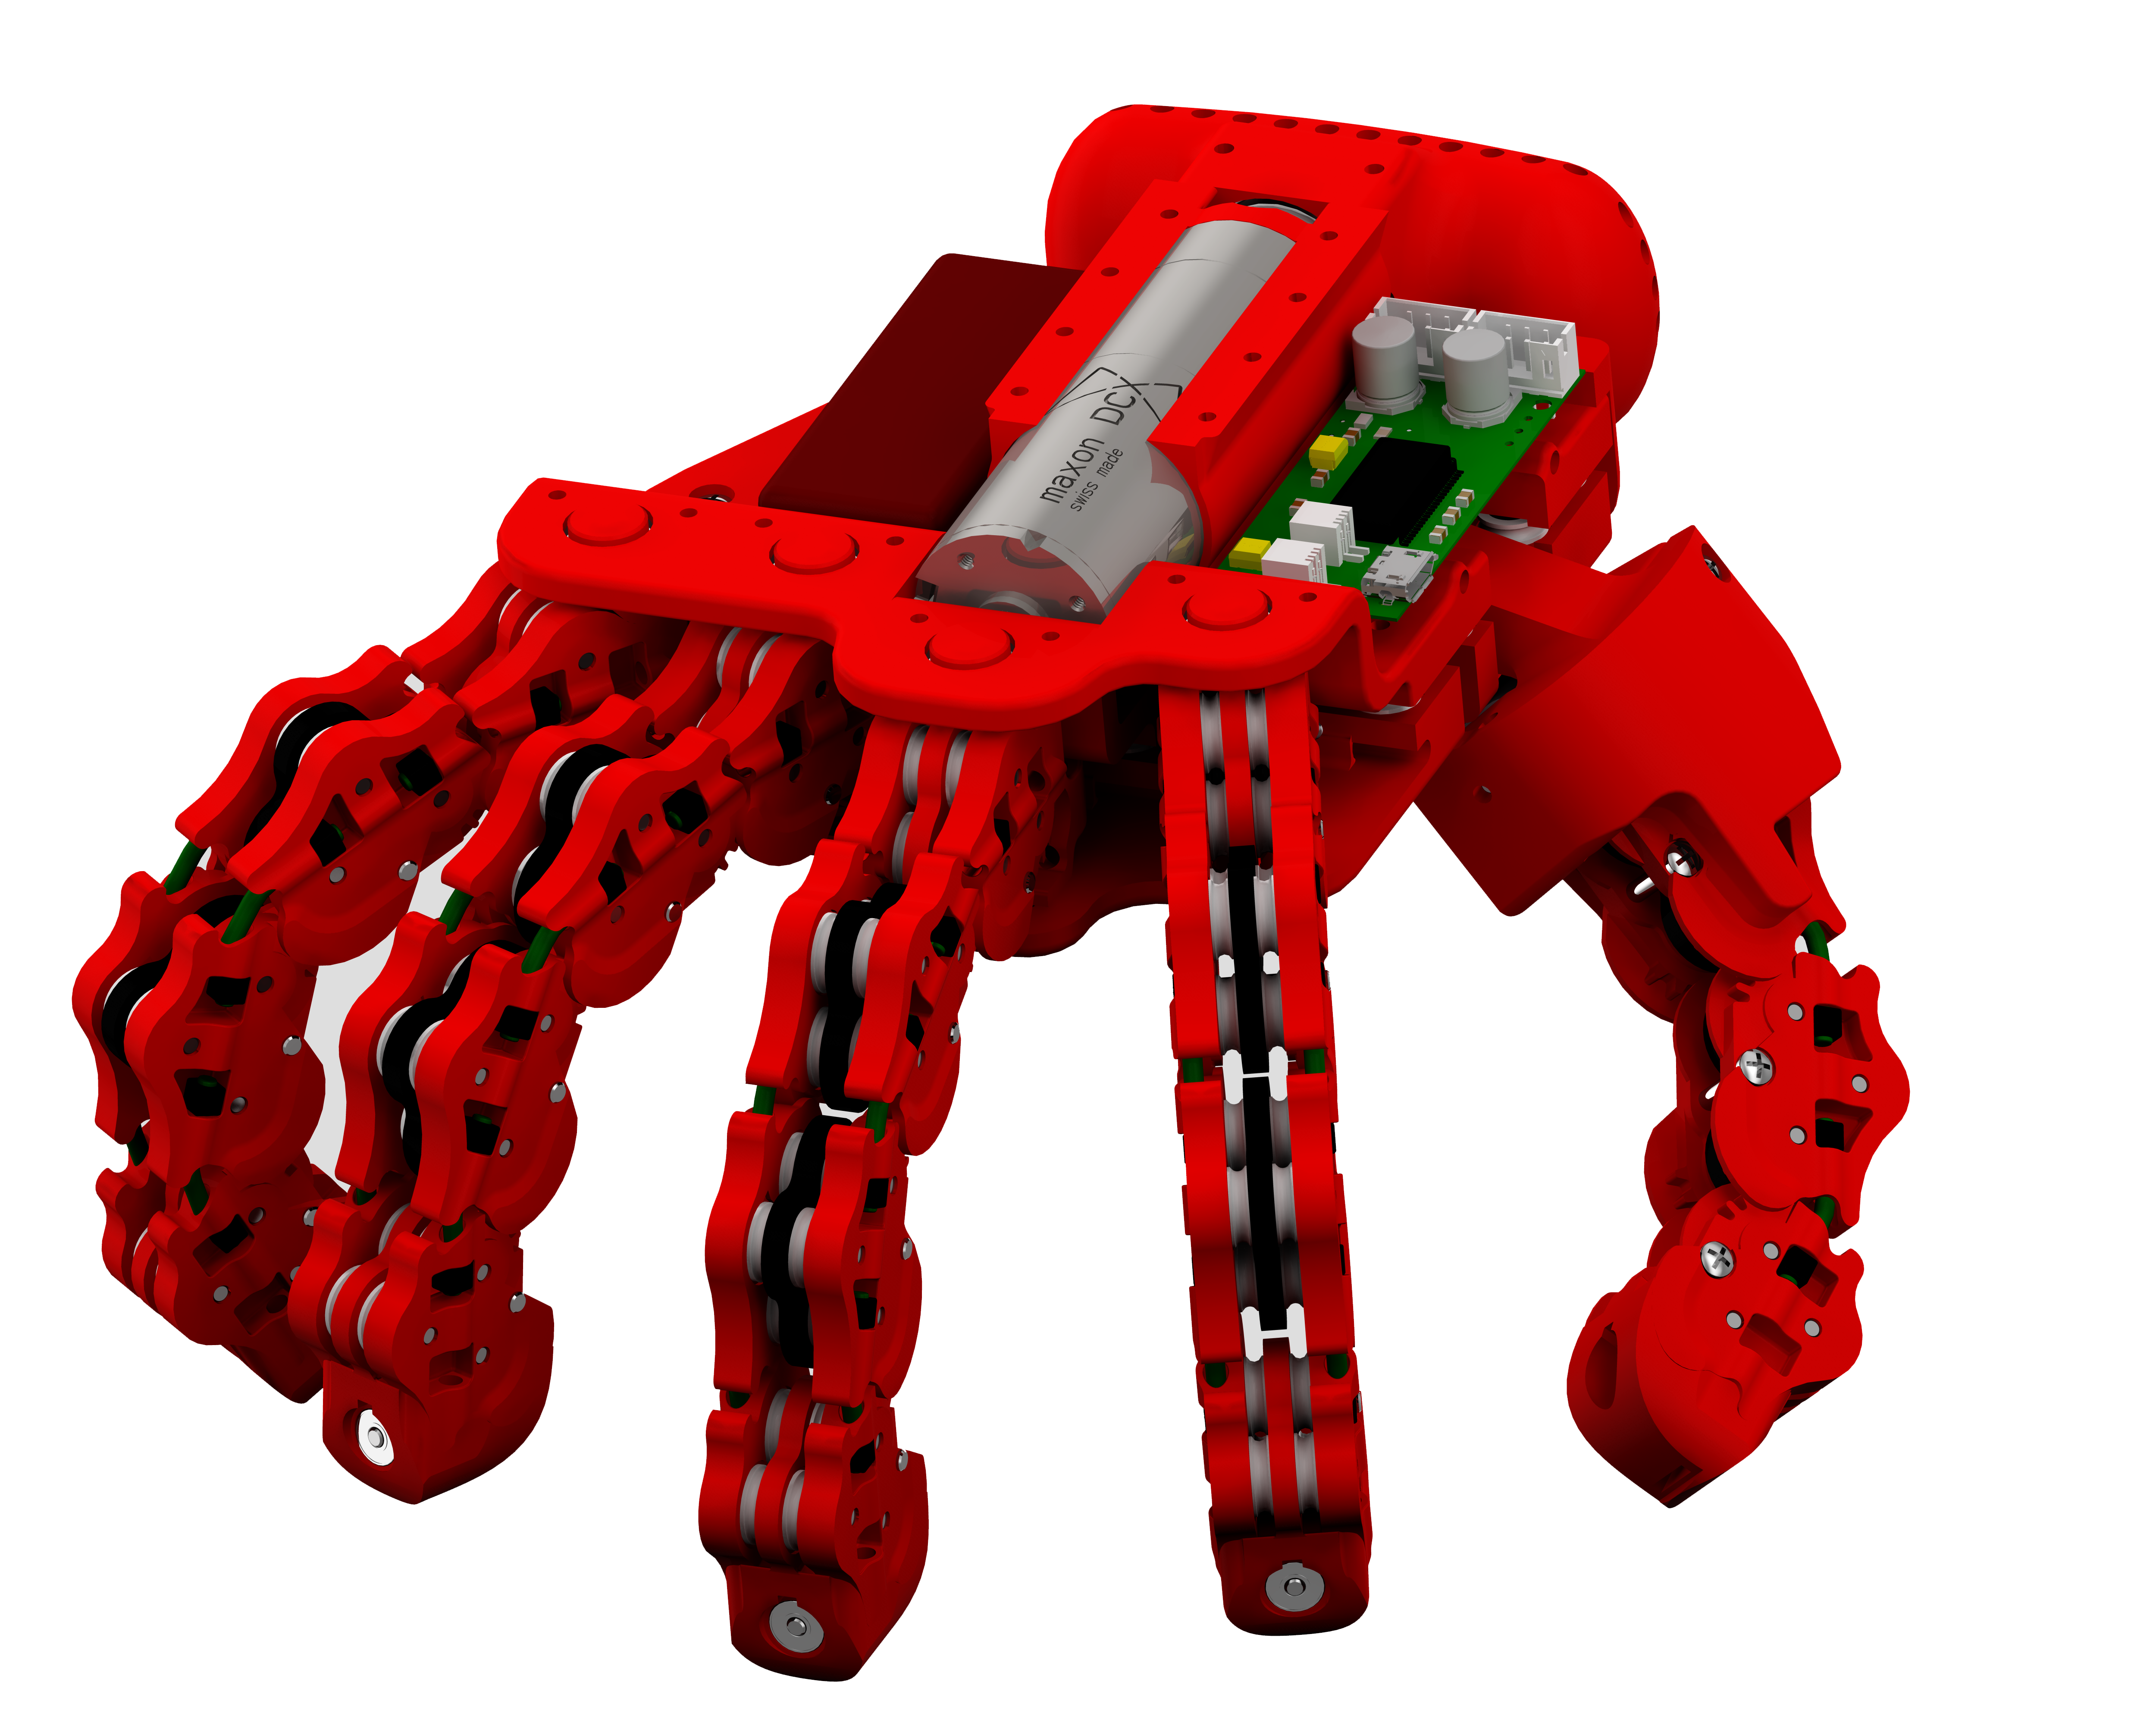
\includegraphics[width=2.5in]{./Graphics/pisa-softhand1}} &
  \adjustbox{valign=m}{\includegraphics[width=2.5in]{./Graphics/pisa-softhand2}}
\end{tabular}
\caption{Pisa/IIT's robotic gripping system, called \emph{SoftHAND},
  takes its design from the structure of a human hand, and is thus
  suitable for every task in which the latter would be. Image courtesy of Manuel Giuseppe Catalano.\label{fig:pisa-softhand}}
\end{figure}

\begin{figure}[htbp]
\centering
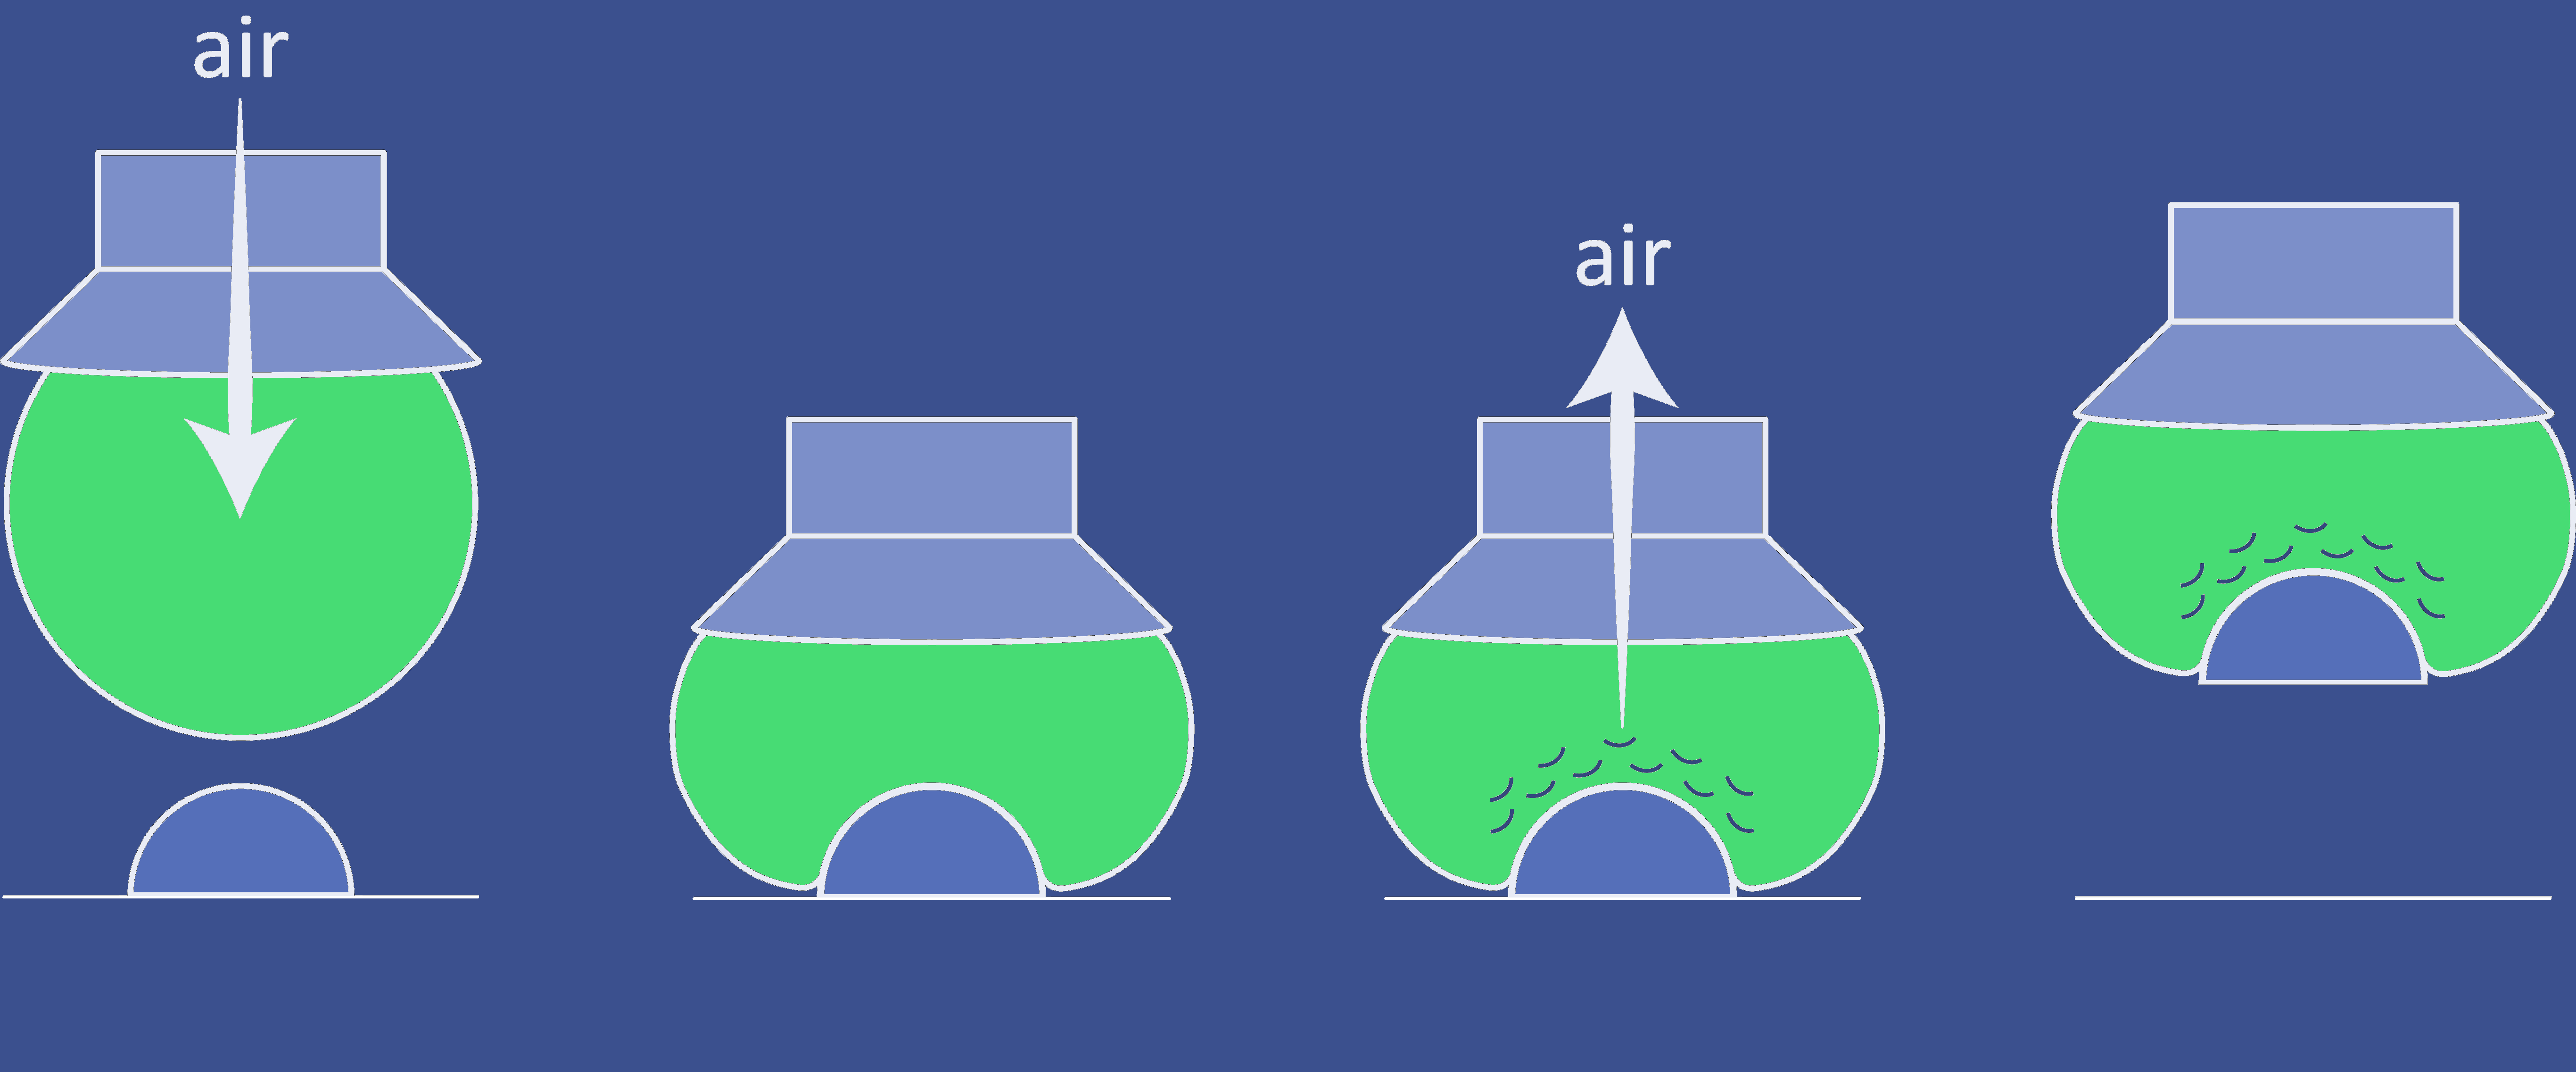
\includegraphics[width=3in]{./Graphics/versaball}
\caption{Empire Robotics' gripping system, called \emph{Versaball},
  diverges from the recent humanoid research and proposes a novel
  approach to the gripping problem. Image courtesy of Bill Culley.\label{fig:versaball}}
\end{figure}

\section{A case study for automated gripping systems: Amazon Picking
  Challenge} \label{sec:apc}
The high request of research in the field of automated objects picking
is not only a supposition, but has been proven to be a impellent need
by the financial effort that big companies are putting on this
topic. One of the most important events which has come out for this is
the \emph{Amazon Picking Challenge}, a robotics competition which saw
its first edition if June, 2015, as part of the 2015 edition of the \emph{IEEE
International Conference on Robotics and Automation (ICRA)}. This
event has brought some of the world's top-level research 
centres to show the state of the art in this field.

Being one of the biggest companies in the world, and establishing its
multi-billionaire business mainly on big volumes on electronic sales
of material goods, Amazon.com, Inc. has important and obvious interest
in selling automatization\footnote{http://www.wired.com/2014/06/inside-amazon-warehouse/}. In fact, during the last years, it has
added more and more automatic processes to their warehouses; in
particular, the whole organizative process, which receives its
material orders directly from the Amazon web selling system, is
managed totally in an automatic way, delivers its orders to the
warehouses, manages the package delivery process, and thus provides
the totality of the order fulfillment service. This huge organization,
however, still relies on a huge manpower (the Phoenix warehouses
consist of an impressive $0.1\unit{km^2}$ structure, employing more
than 1500 people); the long-term plans for it have been made evident
in recent years, being to bring full independance from human intervention for the whole
sales process: in this sense, research has first focused on investing
for the delivery path going from the destination warehouse to the
buyer's address, with the big investment made in 2013 on drones-based
systems, and the 2015 announce that deperible products would have been
made available to the final customer within one hour from order, which
started to work in the early November, 2015, in major world's
cities. As this research projects are quickly converging on a
solution, Amazon started to move on with the last -- and most
difficult -- problem which still has to be solved, which is the one of
internal automatization of warehouses, i.e. moving objects from one
place to the other into the factory and automatically package them,
using if possible the same robot which took the object from its
stocking place.

For this purpose, the contest's specifications have been made quite simple, and the plans
for future editions are to increase the difficulty level of the tasks
to be completed, in order for the best research groups to develop a
stable and robust platform which will be able to substitute the human
manpower almost completely.

The goal of this thesis project is to develop a framework for robotic
gripping like the ones proposed into this challenge; this will be able
to be extended and used as a base to build general-purpose robots
which are the aim of factory automation systems of these types.

The complete source code of this project, which complements this
thesis, together with its documentation, which comes as an integrative part to this more theoretical report, can be found at \url{github.com/Conte91/JG}.

\subsection{Amazon Picking Challenge problem statement} \label{sec:apc}
Here follows a brief description of the Amazon Picking Challenge's
specifications, which have been taken as a reference for how the robot
shall behave in a warehouse environment.

\begin{itemize}

\item{First of all, each robot is assigned a \emph{shelf} on which it will
operate; both the robot and the shelf could actually be able to move
into the warehouse (KivaPOD shelves, for example, are systems able to
move on wheels and coordinate each other in a crowded environment),
but for the purpose of focusing on the problem it will be assumed
that, when instructed to start, the robot will already be in front of
its shelf;}
\item{A shelf is made of several \emph{bins}, for which the location
into the shelf is known a-priori; each bin can contain one or more
instances of objects taken from a predefined set. For this challenge,
a set of 25 items commonly sold on Amazon.com has been selected,
composed mainly by everyday items such as books, children toys, and
office equipment; each object type is uniquely identified by its ID
(multiple objects of the same type share a common ID);}
\item{Each bin is labelled with a sequential letter, starting with A,
and its content in terms of objects is known; what is not known is the
position of these objects inside their bin;}
\item{The list of items which the robot will have to grasp is defined
in a \emph{work order}, which is given as an input to the robot at
startup, as a single JSON file (app.~\ref{app:json} contains an
example of such files); for each item into the work order, both the object's ID and
the bin from which the object has to be taken are specified; it is not
possible that an item does not correspond to a real object into its
bin (i.e. bin descriptions are consistant, and no checks are needed
for this);}
\item{For each item into the work order, the robot will have to
identify the object into the correct bin, pick it, and put it into a
plastic container, representing the destination package of the
object. It is very important that the robot does not break any of the
objects into the shelf while operating, and that it never extracts an
object for the shelf which is not present into the work order (if it
does, it will have to put it back in the correct place); in this
cases, it is preferrable for the robot to do nothing rather than
committing an error.}
\end{itemize}

The rest of this project focuses on implementing a good strategy which
would comply with these specifications; more constraints which have
been included for this work have the rationale of preparing for a
future partecipation in the same challenge for future editions
(starting with the 2016 one). With this in mind, both flexibility and
scalability of the work has been kept in mind for all the design
choices. This led to a software stack that is admittedly more
complex in architecture and usage, but has the advantage of bringing
more complete access to all of its facets for a future user. In this
sense, although a few demonstration softwares have been created, the
scope of this work is more focused on the single components (vision
and gripping algorithms) which will make up the complete system in the
future rather than on the system itself.

\chapter{Detection and fine pose estimation of objects through computer vision}
\label{sec:vision}
\section{Depth cameras' working principles}

The world of computer vision has, in recent years, benefit a lot of new hardware
technologies and improvement. In particular, object pose estimation algorithms
have been developed which, differently from the past ones which based themselves
either on standard, RGB images, or on couples of RGB images to use for
stereoscopic vision, exploit new generations of camera sensors which can provide
3D data to the user. Within the most common types of these are comprehended the
so-called \emph{depth sensors}; these particular kinds of sensors can provide
the user with an image which is built of floating-point, or integer, values,
each representing the distance from the sensor itself to the nearest obstacle
within line-of-sight, along the sensor's axis. If combined with the commonly
used geometric model for a camera, described in detail in sec.~\ref{sec:camera_modelling}, this measurement can lead to having not only a $z$
coordinate for each sampled point, but a complete 3D point $P=(x,y,z)$.

Other known approaches have been used in the past to obtain 3D vision systems:
in particular, the stereoscopic (or \emph{binocular}) system -- i.e., emulating the human vision by usage
of two different cameras -- has been widely studied and used, particularly into
the robotics' field, leading to
results such as \cite{stereo-vision-robot}; using this system, images taken
from two cameras are first scanned for correspondent, influential features
(\emph{keypoints}); pose information for each keypoint is then extracted from
the geometrical properties of the system in what is called \emph{triangulation}
as shown in fig.~\ref{fig:stereo-triangulate}.

\begin{figure}[htbp]
\centering
\includegraphics[width=3in]{./Graphics/stereo-triangulate}
\caption{Two different cameras can match the same feature into different points
of their image: these will allow to extract 3D coordinates for the feature.\label{fig:stereo-triangulate}}
\end{figure}

Anyway, this approach has several limitations and can't be applied for proper
pose estimation of objects. Advantages of using depth sensors instead of
stereoscopic cameras include:
\begin{itemize}
  \item{Stereoscopic cameras can't produce an image with depth information for
      each pixel: in fact, this system is optimised for measuring depth over a
      small subset of the image (the keypoints), while completely ignoring the
      rest of the pixels. This comes as a natural consequence of the fact that
      features must be matched together in order to produce a depth information,
    as points in the background will seldom own such features;}
  \item{Although the previous problem could be solved by only looking for
      objects' keypoints when recognizing them, stereoscopic vision also can't
      be, by nature, as precise as depth sensors; \cite{stereo-precision} has
      shown that in order to have $2\unit{mm}$ of error in depth measurements
      with these systems, one must have precise information about the
      geometrical properties of the searched object, and must apply strong data
      filters in order not to have a high number of outliers; on the other hand,
      good depth sensors such as Occipital's Structure have an average error of
    some fractions of millimetre;}
  \item{Searching for matches into images in order to obtain good precision in
      stereoscopic vision is computationally expensive; also, effectiveness of
      these algorithms suffers from common RGB vision problems such as
    illumination changes or weakly textured images.}
\end{itemize}

Obviously, depth sensors have their disadvantages too: the most problematic one
is usually their very limited range of operation. For example, Microsoft
Kinect's Primesense module can sense in a range going from about $80\unit{cm}$
to about $3\unit{m}$; this makes it useless to adopt a visual depth sensor as
the main vision system in large environments, while stereoscopic vision,
especially if implemented with a high-definition camera, has
virtually no limit (except for focal loss) to the maximum depth it can sense;
this is the main reason for which stereoscopic vision is preferred for
autonomous robots, smart-cities, or search-and-rescue applications. Anyway, this
limited range is adequate for gripping purposes, as the objects will ordinarily
stand fixed within a range of one to two metres from the robotic arm.

For this project, two different type of depth cameras have been used: the first
is Microsoft Kinect, a common camera which can merge together both depth and RGB
informations, widely used in both consumer and research environment,
the layout of which is shown in fig.~\ref{fig:kinect}; the second is Occipital's
Structure sensor, which is a depth-only camera with optimal minimum range
($40\unit{cm}$) and precision capabilities (about $1\unit{mm}$ of maximum error,
with very reduced noise).

\begin{figure}[htbp]
\centering
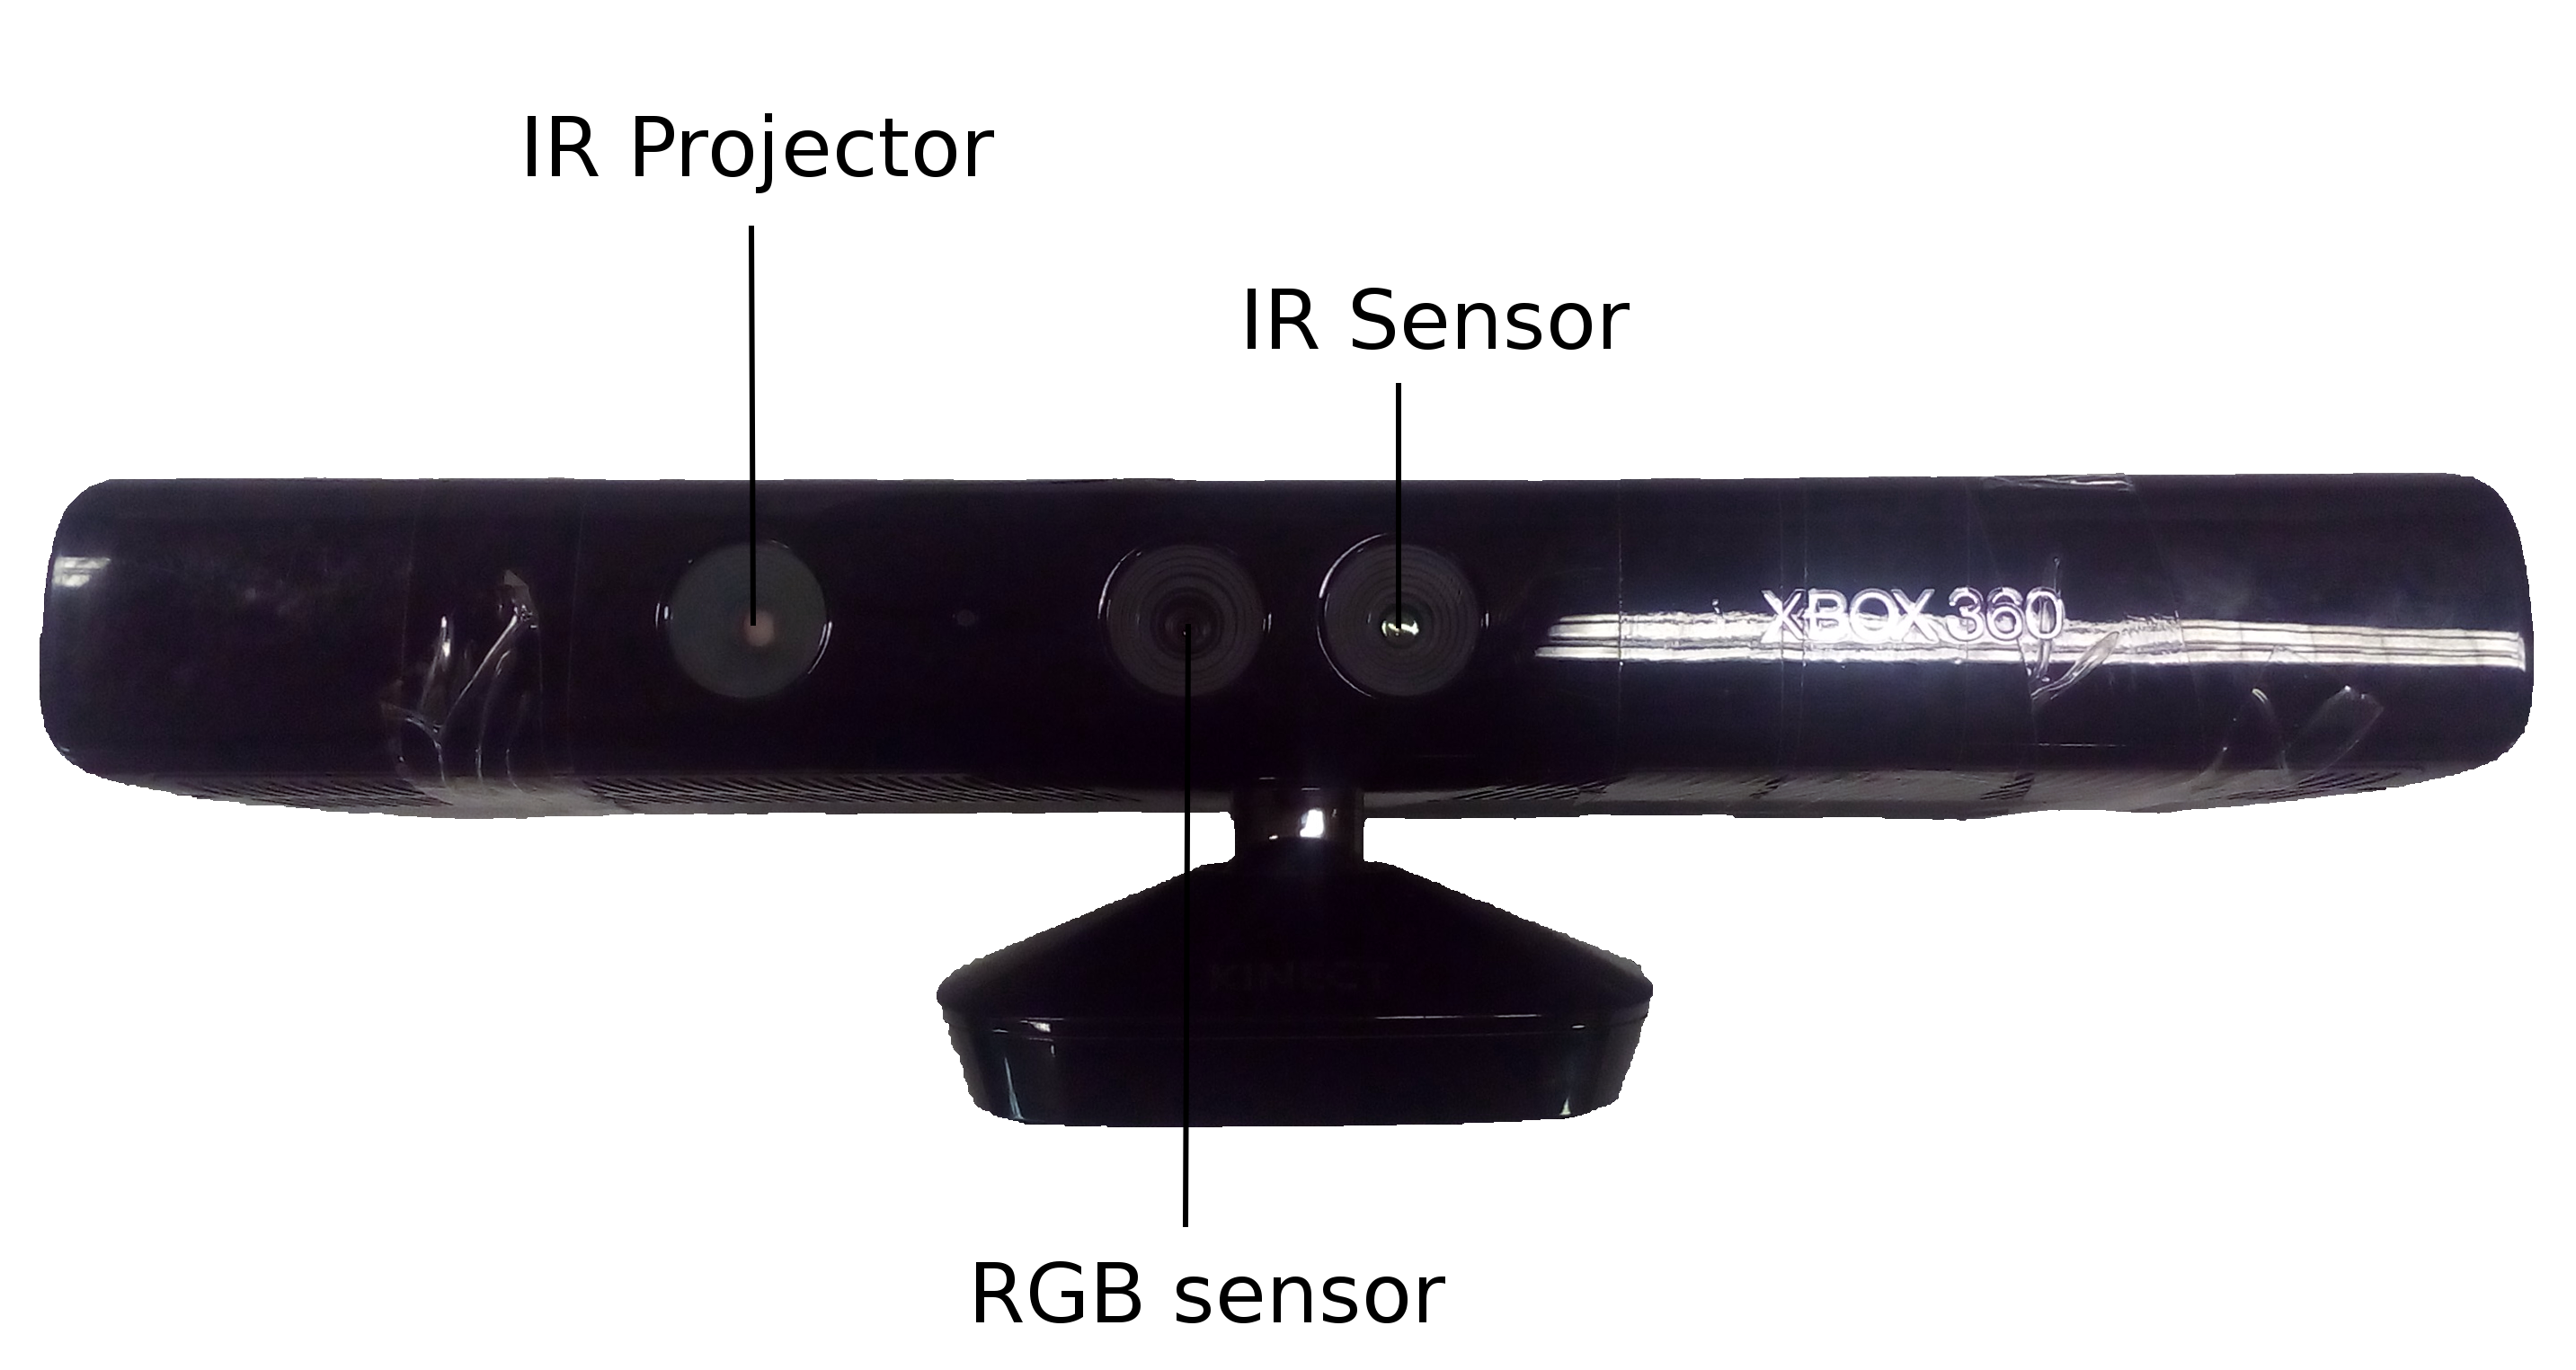
\includegraphics[width=3in]{./Graphics/kinect}
\caption{Microsoft Kinect depth camera, including infrared structured light
projector and sensor, and an RGB camera.\label{fig:kinect}}
\end{figure}

\subsection{Structured light sensors}
In this section, a common type of depth sensor is introduced, which is the one
implemented by Kinect's Primesense hardware, called \emph{structured light
sensor}. This technology was first patented by Shpunt et al. in
\cite{primesense-patent}; although it is used into Microsoft Kinect for its
XBox360 devices, and thus is a mainstream, common device, very few technical
details about the implementation are available. \cite{how-kinect-work}, together
with the original patent's text, remain the best available sources of
information about this kind of technology.

The idea behind structured light sensors is the use of a strong infrared projector
which can draw a known pattern onto the scene. Being made of infrared light,
the pattern will not disturb any RGB camera which is operating in parallel with
it. Primesense devices' projection, in particular, consist in a coherent beam
forming a speckle pattern, as the one shown
in fig.~\ref{fig:primesense-speckle}. When the pattern is projected at a certain
depth, it is distorted by the environment, and its reflected image is sampled
by an infrared sensor (acting like a normal camera), put behind an infrared
filter operating with a narrow frequency range in order to remove noise. All of
the processing described into this section is presented here as a serie of
algorithms, but is in fact implemented in hardware within the Primesense's
processing circuitry. This makes it possible to directly get the depth image in
output, with an extremely good framerate ($30\unit{fps}$ for VGA images).

\begin{figure}[htbp]
\centering
\begin{tabular}{c|c}
  \adjustbox{valign=m}{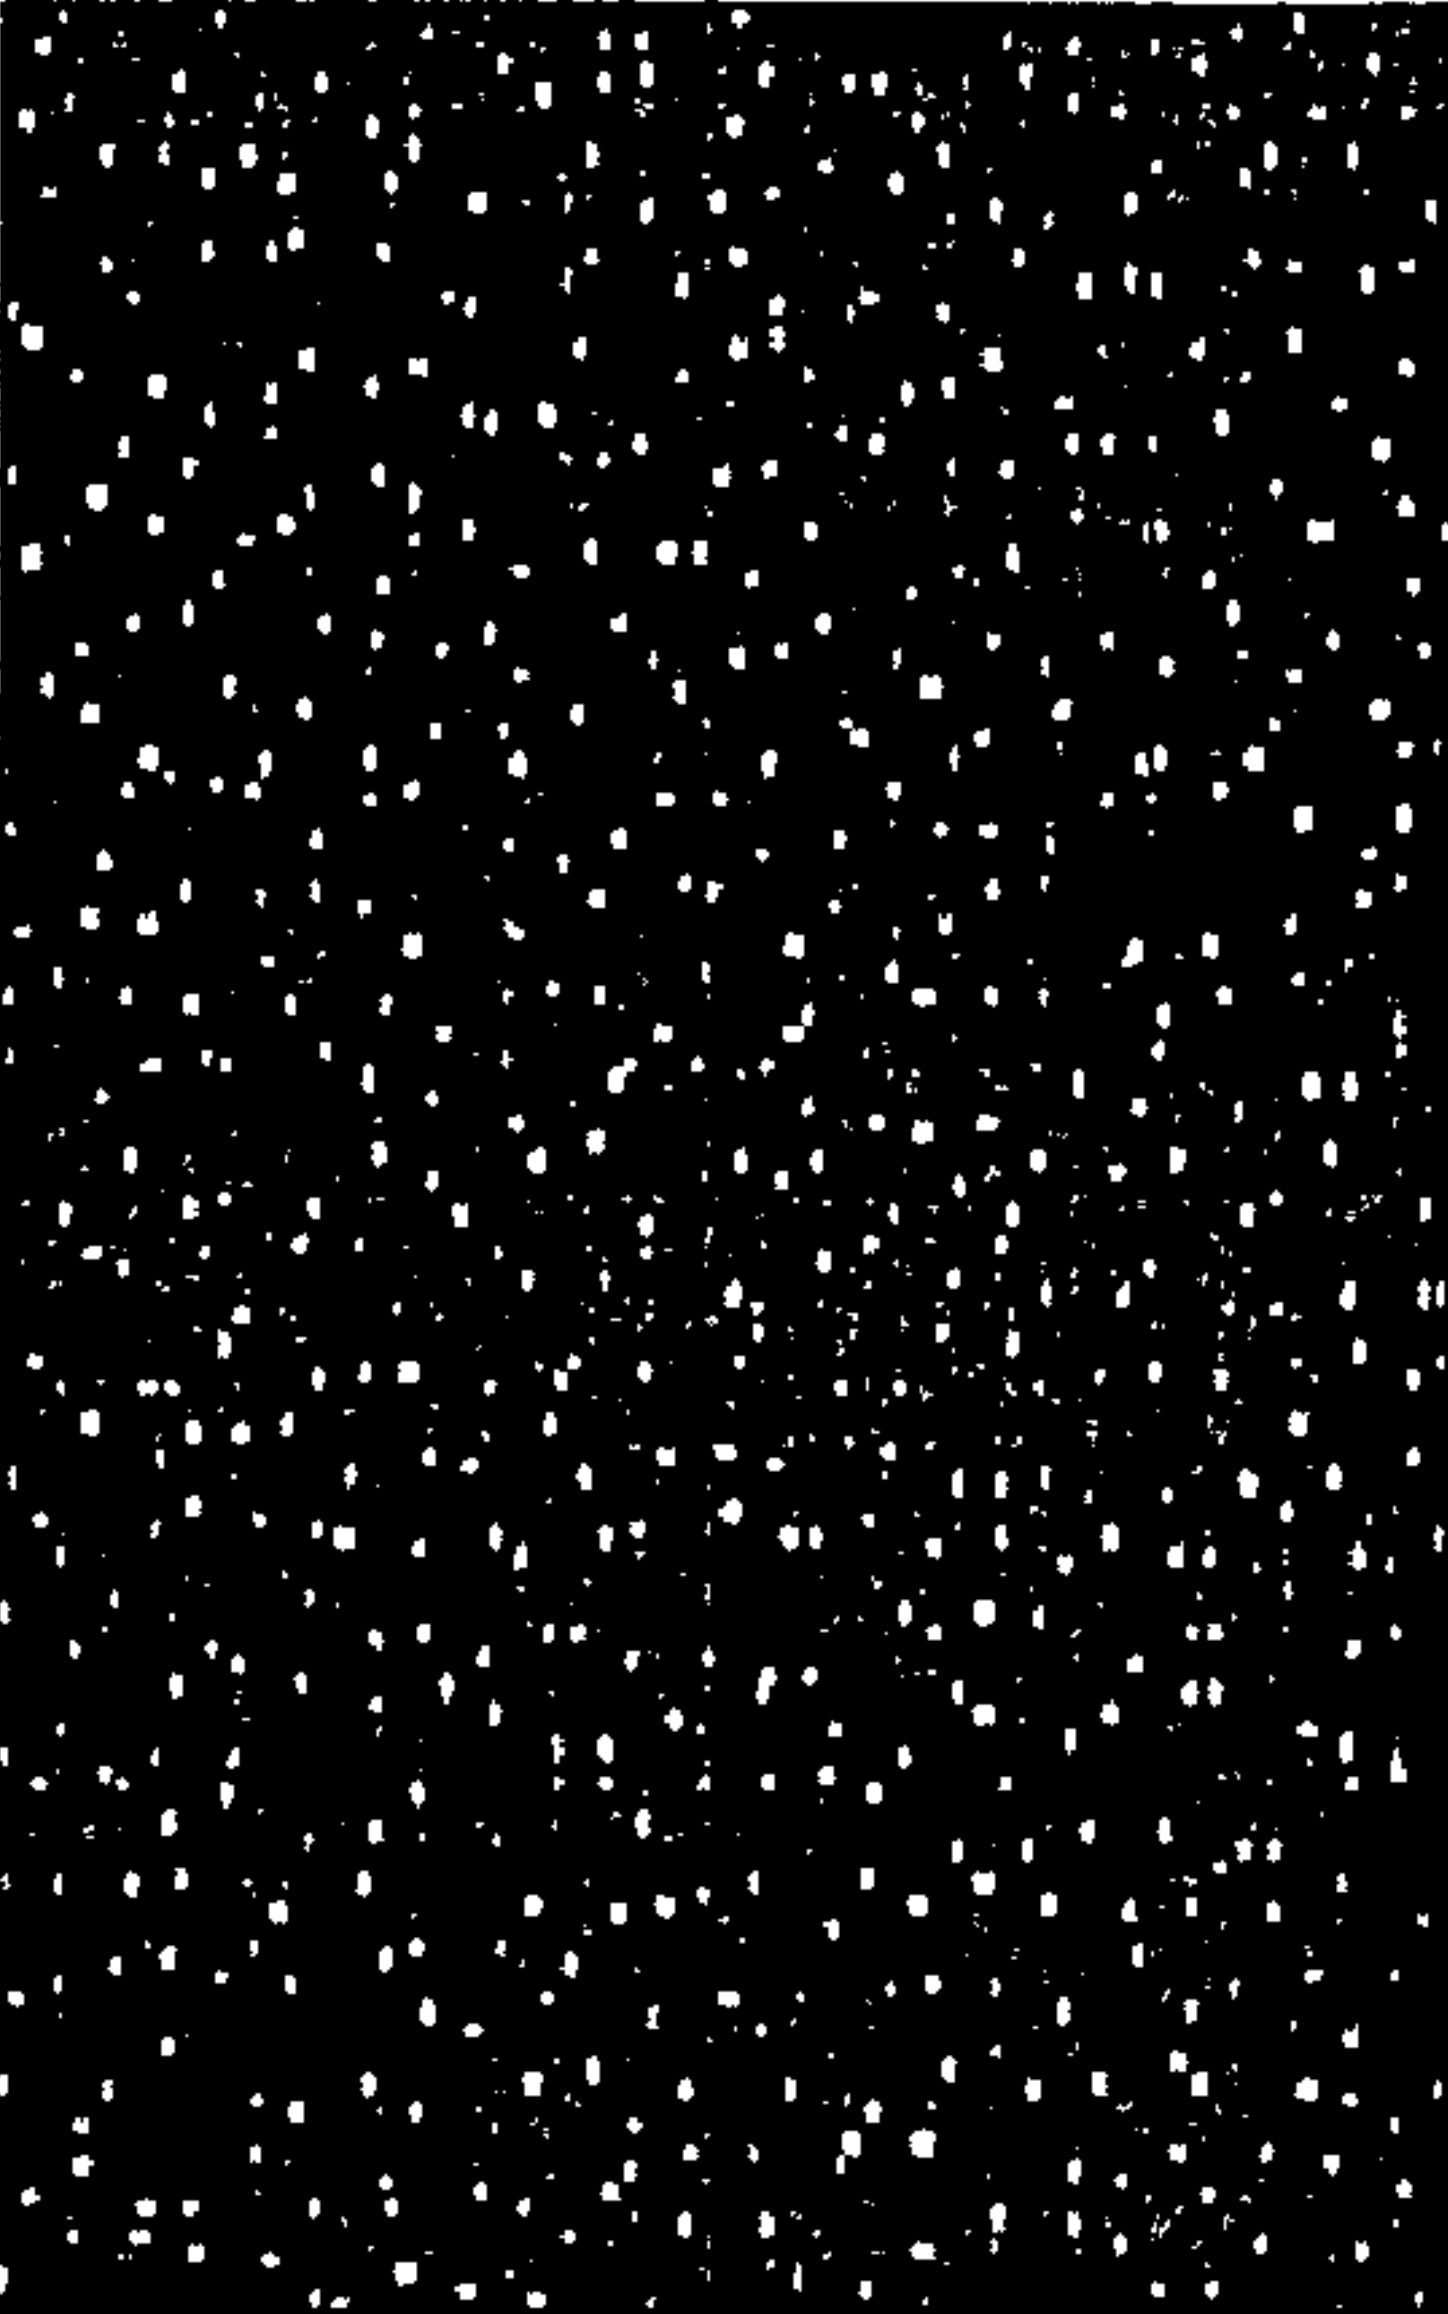
\includegraphics[height=3in]{./Graphics/primesense-speckle}}
&
  \adjustbox{valign=m}{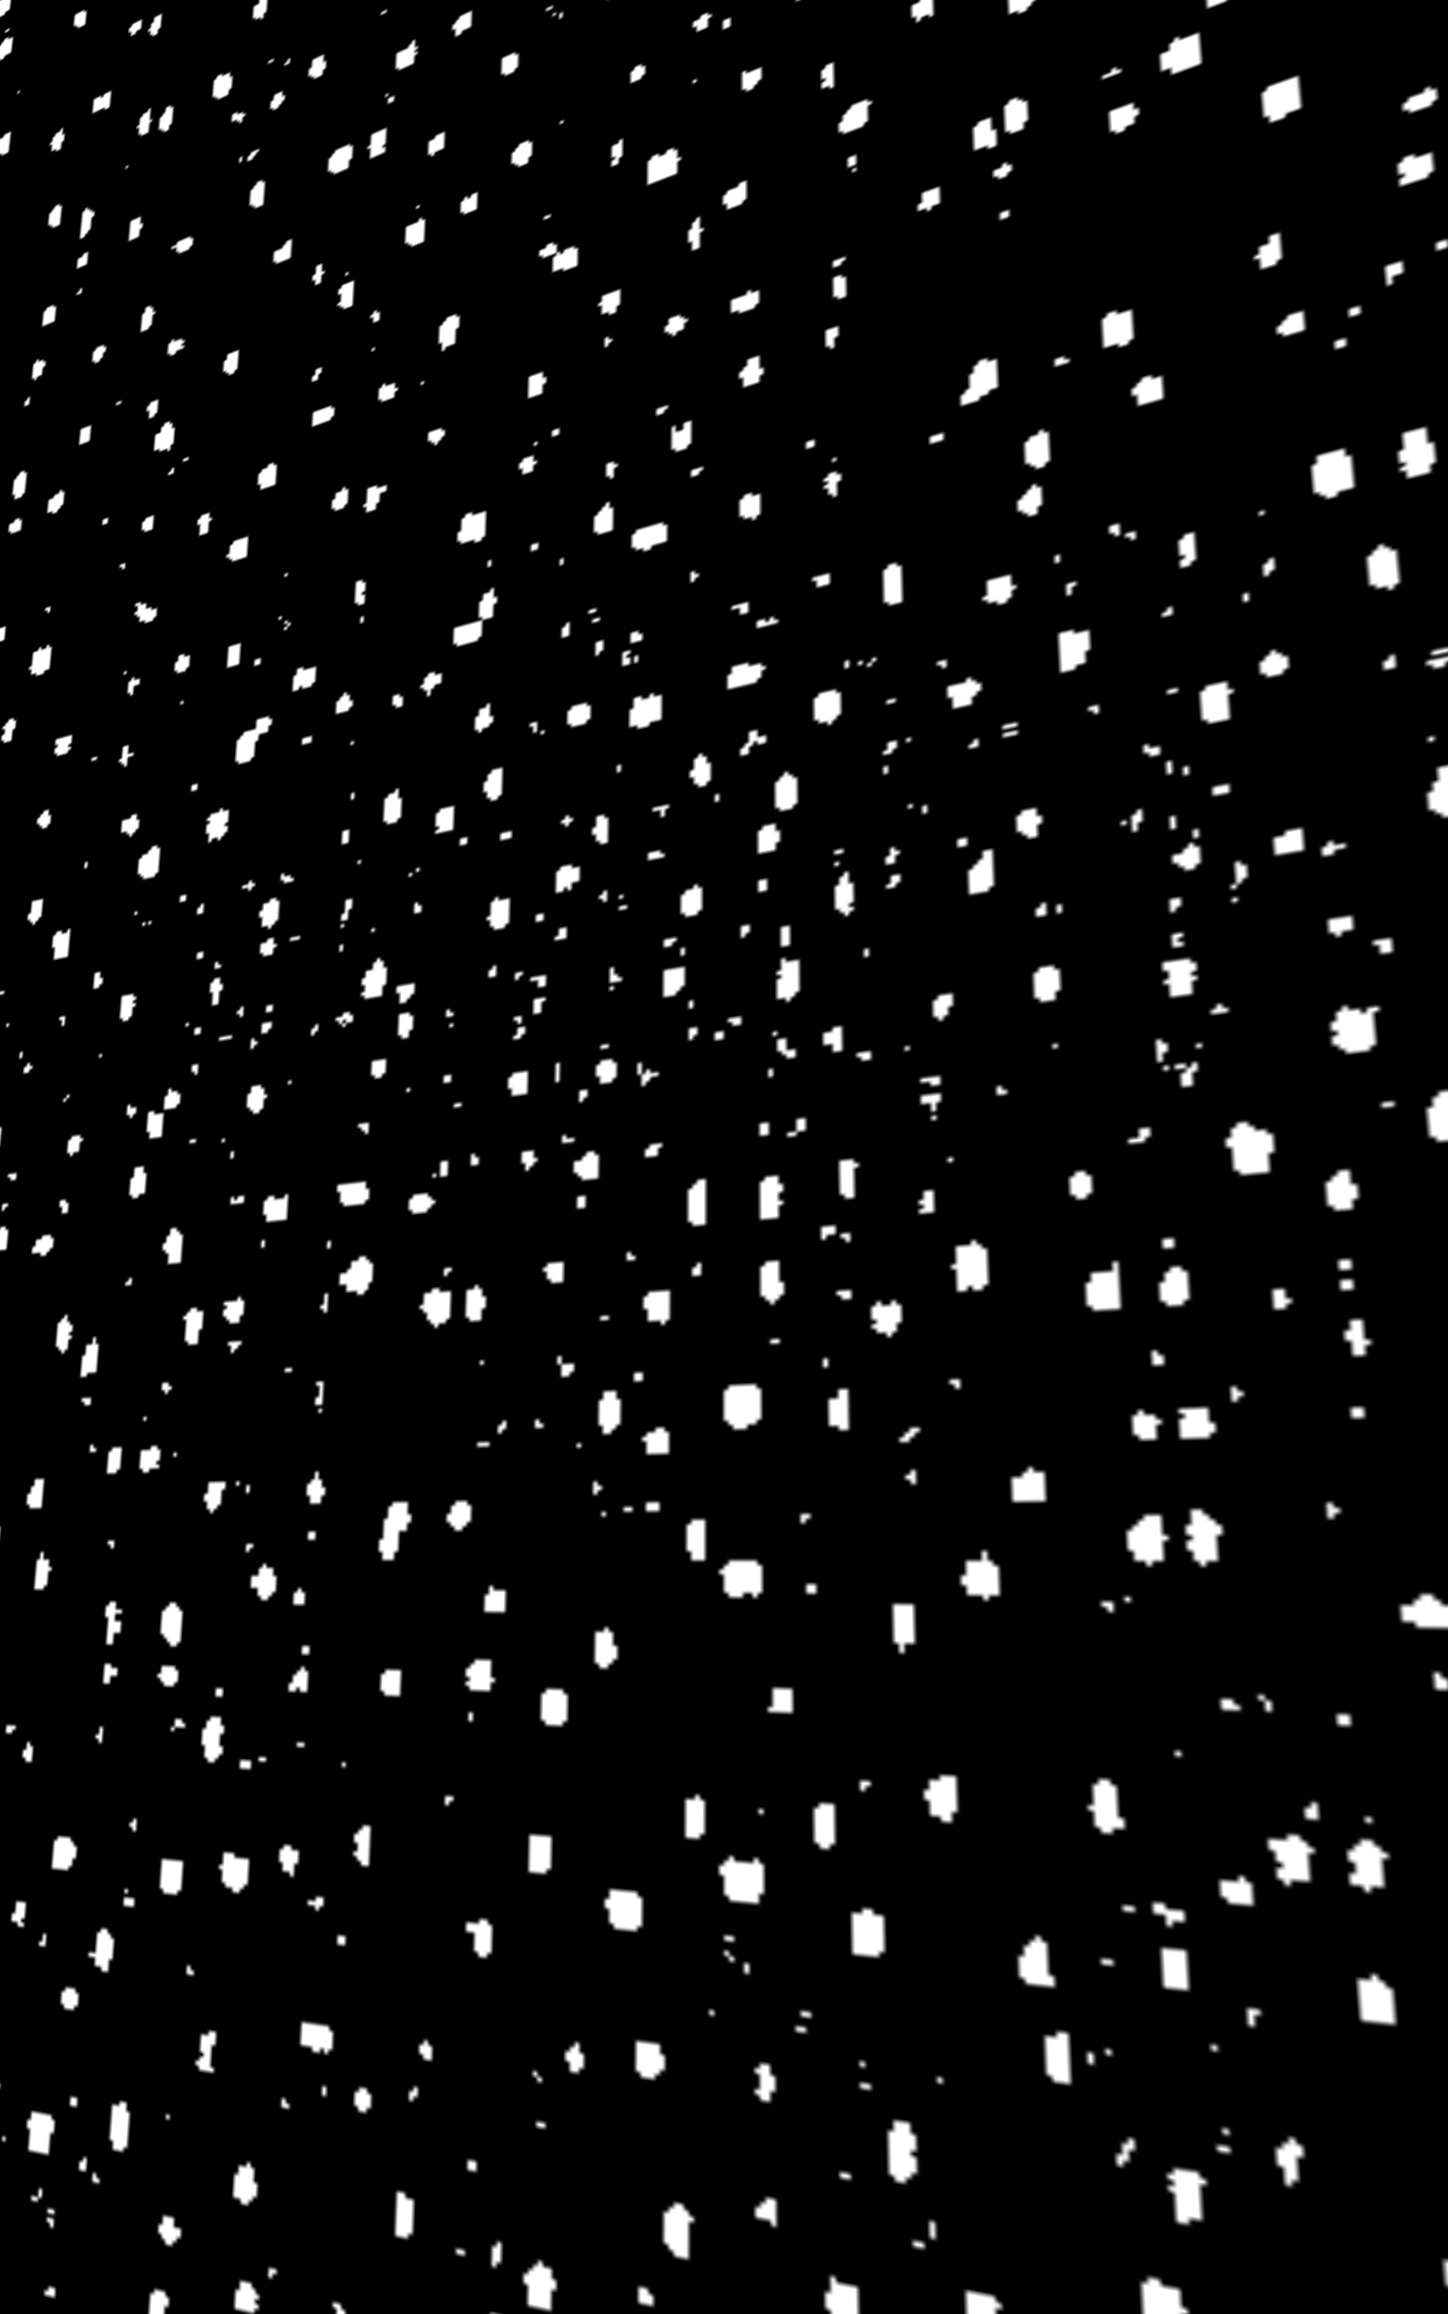
\includegraphics[height=3in]{./Graphics/primesense-speckle-dist}}
\end{tabular}
\caption{Left: speckle pattern, as projected by a Primesense device (from
\cite{primesense-patent}). Right: the same projected pattern, as seen by the
infrared sensor, shows distortion of the pattern depending on the depth of reflection
point.\label{fig:primesense-speckle}}
\end{figure}

Two main techniques are used to obtain a depth value from the sensed infrared
image: \emph{depth from focus}, and \emph{depth from stereo}.

The first one is based on two observations regarding the single spots
composing the pattern: first, as the pattern is both projected
and recaptured using fixed-focus lenses, it will become blurrier the more
distant the reflection point is. Also, lenses used by the capturing device (the
IR sensor) are built in order to have very different focal lengths $f_x$ and
$f_y$ (this concept is explained, together with camera modelling, in sec.~\ref{sec:intrinsics}): they are \emph{astigmatic} lenses. Also, its axes are not
perfectly aligned to the pattern's reference system; in practice, deformation in
the image is introduced by purpose. Usage of astigmatic lenses means that, given
a certain point at a certain depth $d$, it will be more in focus on one principal
axis with respect to the other. The result is that, if a circle of the speckle
is captured using this lens, it will look like an ellipse due to different
blurring on both its directions. The main ellipse's axis angles will vary in function
of $d$.

The second technique used for depth reconstruction is based on the same
principle of stereoscopic vision: as it can be seen in fig.~\ref{fig:kinect}, the projector and the IR sensor are by purpose mounted
at a quite high distance. The result is that each pattern's point is shifted on
one side of the captured image depending on its reflecting distance (i.e. depth
value). Measurement of this shift can improve the results obtained with the
\emph{depth from focus} technique. In fact, this is equivalent to using two
cameras together, in parallel with the depth sensor; the other camera is a
virtual one, as it doesn't match a real sensor: as the pattern image is fixed,
it can be thought of by applying normal stereoscopic matching algorithms with
the captured image and the orthographic drawing of the pattern. This last image
will correspond (for any depth) to the image that would be captured by a camera
placed in correspondence of the projector. With this in mind, stereoscopic
vision can be emulated with a single camera. 
Two advantages are there, with respect to binocular systems: first, no
geometrical calibration is required. Calibration of the sensors' position can be
done once at the factory of origin, and after this it will not suffer from
carriage or system reimplementation, as the sensors are embedded into one single
device. Also and most important, having a fixed pattern to detect extremely
simplifies the problem of features' matching. Features' positions can be
precomputed, and being mainly circular, they are easy to detect in the dynamic
image grabbed by the IR sensor. Knowing their fixed position, triangulation is
almost immediate too.

By combining these two techniques depth can be refined accurately for each
pixel. Most importantly, outliers can be totally filtered out as they will
correspond to very different outputs coming from the first and the second
algorithm; this is a good improvement over binocular systems.

After getting a good point map, the camera model of sec.~\ref{sec:camera_modelling} is used by the camera's hardware to associate to each
obtained spatial location a point into the RGB image taken by the colour sensor.
Again, this procedure is highly simplified by the fact that the relative
position between the two sensors is known a priori. The result of this operation
is what is called a \emph{registered RGBD image}, i.e. an image with four
channels, representing red, green, blue, and depth components of each pixel.

Simplification of the algorithms due to the fixed pattern is the main idea that
allows an efficient implementation of these in hardware; structured light systems are thus
naturally suitable for high frame rates, low cost, high precision depth
measurement solutions.

\section{Camera modelling} \label{sec:camera_modelling}
A central problem when working with camera-generated images and 3D models is
correctly mapping 3D points in camera (and world) frames into 2D points on the
acquired camera's image and viceversa. In particular, the capability to map
points of the world to a generalized camera model in a realistic way allows all
the algorithms, such as point cloud alignement, to work within a generalized,
global coordinate system, which remains valid also if cameras are moved around
within the scene and is camera-independent: this means that different cameras
can be used in order to maximimize the peculiarities of each. Also, virtual
renders can be done using the same model in order to correctly template-match
the chosen data.  A \emph{pinhole} camera model can be used for this task, and
provides the correct approximation for both RGB cameras and depth-capable ones.

\subsection{Pinhole model for registered RGBD cameras}\label{sec:intrinsics}
A camera, be it a digital camera or the human eye, can be modeled by
considering the path the light coming from a point will take when
captured. By approximating the camera's objective with a single point (hole),
light rays come onto projective plane (where the light sensor is) with central
simmetry with respect to the position of the point in world coordinates. By
rotating the $(u,v)$ reference frame of the image so that it has the same
orientation as the image seen by the camera \footnote{Notice that the image
  coordinate system the $V$ axis is pointing downwards; this is coherent both
  with standard screen coordinate systems, which have the origin in the
  upper-left corner, and with having the camera $Y$ axis pointing downwards and
$Z$ axis pointing forward.}, the point corresponding to the camera hole
becomes the destination point for all the light paths, as seen in single-point
prospective. This transformation is called \emph{perspective projection}.

\begin{figure}[htbp] \label{fig:pinhole_camera}
\centering
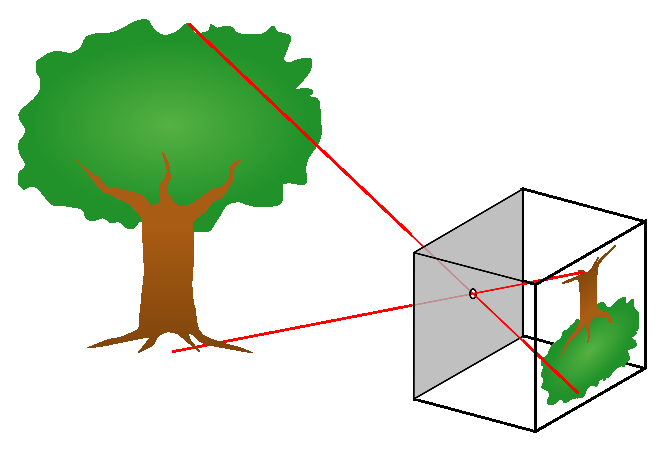
\includegraphics[width=2.5in]{./Graphics/pinhole_camera}
\caption{The pinhole camera model}
\end{figure}
\begin{figure}[htbp] \label{fig:intrinsics}
\centering
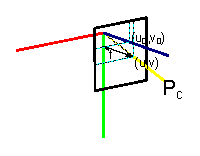
\includegraphics[width=2.5in]{./Graphics/camera_intrinsics}
\caption{Geometric projection of a general point into the camera's projective
plane.}
\end{figure}
Examining the geometric properties of this system from fig. \ref{fig:intrinsics}, we can easily extract the
transformation from a point $P_c(x_c,y_c,z_c)$ in the local coordinate system
$X_cY_cZ_c$ to the corresponding point $P_p(u,v)$ in the image's coordinate
system by applying trivial similar triangles' laws:

\[
  \begin{array}{c}
    \left\{\begin{array}{c}
    \frac{(u-u_0)}{\lambda _x f}=\frac{x_c}{z_c} \\
    \frac{(v-v_0)}{\lambda _y f}=\frac{x_c}{z_c}
  \end{array}
  \right. \\
  \Updownarrow \\
  \left\{\begin{array}{c}
      u=\left(\frac{x_c f}{z_c}\right) \lambda _x+u_0 \\
      v=\left(\frac{y_c f}{z_c}\right) \lambda _y+v_0
    \end{array}
    \right. 
  \end{array}
\]

Here, $\lambda _x$ and $\lambda _y$ are camera-dependant ratios between the
physical sensor's dimensions and its horizontal and vertical resolution, in
order to map coordinates from meters to pixels. These can be merged into $f$ to
get $f_x$ and $f_y$.

Also, as we are assuming to work with a registered RGBD image, $z$ coordinate is
directly measured from the depth sensor and is reported on a per-pixel basis
without the need of further processing.

If we use \emph{homogeneous coordinates} % TODO nota
to describe both 3D and 2D points, we get

\begin{equation} \label{eqn:intrinsics}
z_c \left(\begin{array}{c}u\\v\\1\end{array}\right)
  =
  \left(\begin{array}{cccc}
      f_x & 0 & u_0 \\
      0 & f_y & v_0 \\
      0 & 0   & 1 
  \end{array}\right)
\left(\begin{array}{c}x_c\\y_c\\z_c\end{array}\right)
\end{equation}

We call the matrix 
$K=
  \left(\begin{array}{cccc}
      f_x & 0 & u_0 \\
      0 & f_y & v_0 \\
      0 & 0   & 1 
\end{array}\right)$
the \emph{intrinsic} camera matrix. This matrix incorporates all the
characteristics which are proper of the used camera, and is different for each
camera -- also of the same model -- as it depends on small build details too,
such as lens geometry.

\subsection{Global camera transformation}
By using the matrix derived in section \ref{sec:intrinsics}, points from 2D
images can be brought into a reference system centered into the camera.
By considering the relative transformation between the world's frame and camera
frame, we can move those points into global coordinates to be further
manipulated from other algorithms in a camera-agnostic way.

If we consider $E$ to be the relative pose between world and camera, we have
(again, using homogeneous coordinates):

\begin{eqnarray}
  E&=&\left(
  \begin{array}{c}
  R | T \\
  0 | 1
\end{array}
\right) \\ 
\nonumber \\
\left(\begin{array}{c}x\\y\\z\\1\end{array}\right)
  &=&
  E
\left(\begin{array}{c}x_c\\y_c\\z_c\\1\end{array}\right) \label{eqn:extrinsics}
\end{eqnarray}

The matrix $E$ is called \emph{Extrinsic camera matrix}.

\subsection{3D cloud reconstruction from RGBD image}
By inverting equations \ref{eqn:intrinsics} and \ref{eqn:extrinsics} we can pass from homogeneous
$(u,v,z_c)$ coordinates to homogeneous $(x,y,z)$ coordinates. In practice, this
means passing from points into a camera-generated image to a cloud of points in
the global coordinate system.

\begin{equation}
  \left(\begin{array}{c}x\\y\\z\\1\end{array}\right)
  =E^{-1}K^{-1}\left(\begin{array}{c}u\\v\\z_c\end{array}\right)
\end{equation}

\subsection{Calibration of camera parameters}
Calibration is the process of extracting the intrinsic and extrinsic
camera matrix for a camera. It is done through the analysys of a serie of RGB and depth
frames containing a single, known object with known size and features. In
particular, a big chessboard pattern has been chosen for this work.

Intrinsic camera matrix can be obtained by using the built-in
\texttt{calibrateCamera} OpenCV's feature %TODO ref
. Before calling it, the pattern's features can be found using the corresponding
facilities like \texttt{findChessboardCorners}. This function examines a serie
of $(u,v)$ points corresponding to the features as they are seen from multiple
frames and multiple pattern's poses, and tries to minimize the RMS error on a
fitness function considering the relative position between these features. Care
must be paid in order to cover the whole camera space when taking frames, thus
minimizing the total error on the intrinsic matrix computation.

In order to compute efficiently the extrinsics matrix, an original program has
been developed in order to exploit depth information too, which is not used at
all by OpenCV's builtins. First, the chessboard corners are located using the RGB
channels of the image. After this, they are sorted so that the point with the
lower $u$ and higher $v$, i.e. the one in the bottom-left corner, is point
number 0, and proceeding left to right. Each point is then mapped to its 3D
camera coodinates $(x_c,y_c,z_c)$ using equation \ref{eqn:intrinsics}. 

Points associations between camera and global coordinates are done
bidirectionally: point 0 is associated to global origin, and point N to global
coordinate $(x_n, y_n, 0)$.

As points' correspondances are univocal, we can use the ideas presented in
\cite{extrinsics-algorithm}, which introduce a closed-form algorithm for finding
the optimal transformation between the points. First, we find the two points sets' relative
translation by computing the distance vector between the points' centroids:
\begin{equation}
  T=\frac{1}{N}\sum_{i=1}^{N}(P^i-P_c^i)
\end{equation}

After this, we align the two centroids into the origin and use Singular Value
Decomposition to find the optimal rotation:
\begin{eqnarray}
  H &=& \sum_{i=1}^{N} (P^i - C)(P_c^i - C_c)' \\
  \left[U,S,V\right] &=& SVD(H) \\
  R &=& VU'
\end{eqnarray}

Finally, the error can be computed and tested to be low enough. If the result is
good, the theoretical and captured chessboard are correctly aligned as shown in
fig. \ref{fig:extr_alignment}.

Both intrinsic and extrinsic matrices are saved to a camera model file by the
calibration programs.

\begin{figure}[htbp] \label{fig:extr_alignment}
\centering
\begin{tabular}{c|c}
  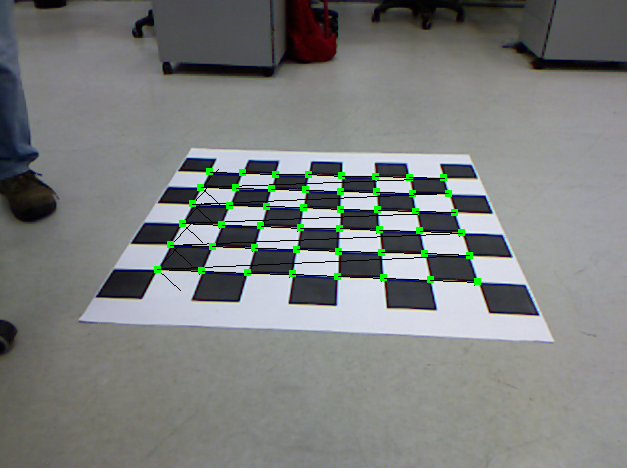
\includegraphics[width=2.5in]{./Results/Chessboard_points_cut} &
  \raisebox{-.5\height}{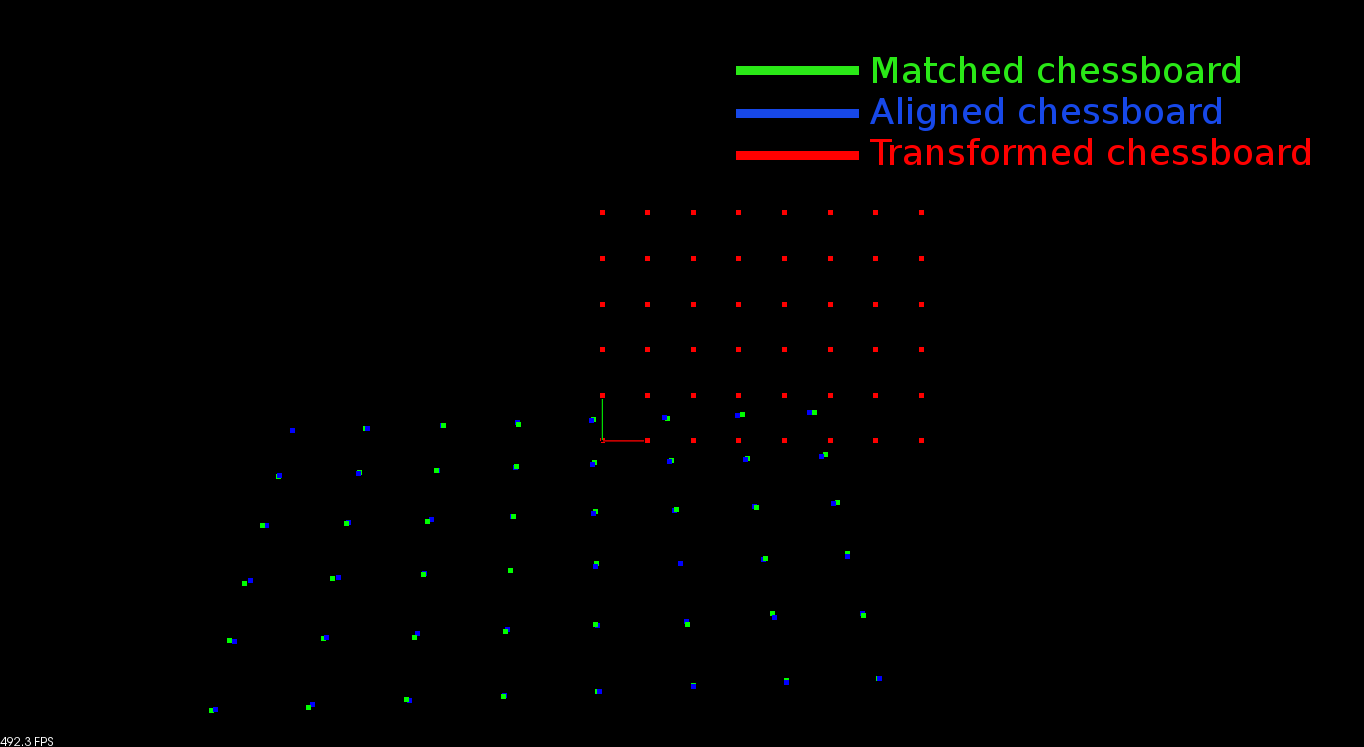
\includegraphics[width=2.5in]{./Results/Chessboard_alignment}}
\end{tabular}
\caption{Left: Chessboard's points are correctly found during calibration. Right: Chessboard's points are correctly aligned after full camera calibration.}
\end{figure}

\section{OpenGL rendering process} \label{sec:opengl-rendering}
In order to obtain good renderings for training and recognition purposes, it is
important to create photo realistic, virtual snapshots of the objects in
diffent poses. It is also important to use the same model of camera introduced in sec.
\ref{sec:camera_modelling} in the most uniform manner as possible.

In this section, this modelling is described. First, a brief
introduction to OpenGL (sec. \ref{sec:opengl-intro}) and to the correct usage of homogeneous coordinates (sec.
\ref{sec:homogeneous-coordinates}) is done, followed by a description of OpenGL reference systems (sec.
\ref{sec:opengl-reference-systems}). After this, the OpenGL rendering
process is analyzed more in details (sec. \ref{sec:opengl-rendering-process}), and finally the
implementation of objects' rendering for the purpose of this project is
described keeping all of the previous into account (sec. \ref{sec:renderer3d}).

\subsection{Homogeneous coordinates} \label{sec:homogeneous-coordinates}
Homogeneous coordinates were introduced by the famous mathematician August Ferdinand Möbius in
\cite{homogeneous-coordinates}; they are a common way to represent points in
\emph{projective geometry} by using an additional scale value, usually called
$w$, in represented
vectors, which can be seen as an inverted scale factor for the whole vector. In
practice this means that the association between homogeneous coordinates $H$ and
cartesian coordinates $C$ is:


\begin{equation}
H=\left(\begin{array}{c}wx\\wy\\wz\\w\end{array}\right) \Leftrightarrow
C=\left(\begin{array}{c}x\\y\\z\end{array}\right)
\end{equation}

Although this generates redundancy, as there will always be more freedom degrees
then constraints when mapping from coordinates to points (2D points are
represented with 3 values, 3D points with 4, and so on), this notation can
simplify a lot the computing effort for usual geometric operations -- for
example, scaling a set of points only requires to change their $w$ value.
Also, when performing matrix operations, this geometry has the good property to
be \emph{scale-invariant} for vectors, which means that coordinates are
multiplied by a constant value they keep representing the same point.

The last interesting property of homogeneous coordinates for the purposes of
this thesis is their capability to easily distinguish points from directions;
in fact, a directional vector can be represented as a point at the infinity,
and, differentely from cartesian coordinate systems, homogeneous coordinates
easily represent them as directional vectors by setting their $w$ coordinate to
$0$.

Also, \emph{all} affine transformations, if operating on homogeneous
coordinates, can be representing as $4\times 4$ matrices including rotation
matrix $R$, translation vector $T$, and scale properties $s$:

\begin{equation}
  A=\begin{pmatrix}
    R & T \\
    0 & s
  \end{pmatrix}
\end{equation}

By representing directional vectors as points at the infinity, they will have
the good property of never being scaled nor translated by these transformation,
which is desirable e.g. for unit direction vectors.

OpenGL, together with applications like OpenCV and algebraic libraries like
Eigen\footnote{eigen.org}, use homogeneous coordinates for almost all of their
work. During this project, homogeneous coordinates have been used extensively
thanks to the Eigen library, in order to have a well-defined system (Affine
transformations) to define the reference systems of interest, and in order to
compute transformations between objects. Homogeneous coordinates are converted
to native formats (e.g. COMAU robots' euler axis representation) only in the
final backend of the applications, so that data representation is unique and
coherent in the whole scope of the project.

\subsection{OpenGL reference systems} \label{sec:opengl-reference-systems}
Opposing to a lot of 3D manipulation systems, such as COMAU's robotic arms or
CAD applications, which use different coordinate systems for different logical
aspects of their work, typically requiring at least a \emph{local} and a
\emph{global} coordinate system, OpenGL only works with a single 
coordinate system (\emph{clip coordinates}) when drawing (rendering) objects,
in which camera's frame is fixed at the origin and aligned with global axes,
with Z-axis pointing backward\footnote{This actually brings out a left-handed
  coordinate system, which must be taken into account when interfacing OpenGL
with external world like it has been done in this project.},
which is then transformed into another unique coordinate system
(\emph{Normalized device coordinates}) after drawing in order to map 3D points to 2D points into the
render (camera) buffer. A third buffer (\emph{Z-depth buffer}) keeps
informations about the depth of drown points into the visible scene and is
registered with the rendering buffer. As described in \cite{opengl-book}, in order to give the
programmer full access capabilities to the rendering engine's internals, 
multiple reference systems appear to the user only on the
OpenGL API's abstraction layer, in which different functions \emph{appear} to
work on different coordinate systems, but instead limit themselves to act
differently on the latter. Thus, with the target of emulating a physical
camera in mind, the programmer can act on the most suitable components of the
rendering process as needed, without caring about what is the right coordinate
system to transform. 

\subsection{Details about OpenGL rendering process} \label{sec:opengl-rendering-process}
Here follows a description of the full process performed by OpenGL in order to
render a 3D mesh, from scene generation to actual mapping of 3D points into a
2D buffer. A complete and detailed description can be found in
\cite{opengl-book}, completed of actual API examples which are omitted here
for brevity.

OpenGL library implements a state machine: sequential calls to library
functions modify internal state variables (e.g. colour information), allowing the renderer to be
instructed about how to add elements in the scene and how to transform them to
get the final renderer. Thus, single, independent objects can draw themselves
into the scene and manage each one a single part of the scene (e.g. camera and
fog): current scene's state is actually a global accessible datum. While this
has the obvious advantage of full and deep freedom of implementation, it also
brings the drawback of needing to be careful for how each of the elements
modifies the global state when it finishes operating. In general, it is thus
important to define with extreme precision what each object is supposed to do
and never implement complex operations in a single block, rather splitting them
into single, well-defined tasks.

In this project the simpler -- although deprecated in newest (3.0) versions and
substituted by shaders --
rendering procedure using OpenGL's \emph{fixed pipeline} has been used; this
procedure assimilates the rendering process to an assembly line, in which every
element of the scene undergoes a predefined sequence of processing steps before
being merged with others to form the final render. In particular, geometric data
like lines or polygons are moved into the scene, cut based on their $z$ coordinate, and
finally mapped to 2D screen coordinates through the \emph{projection matrix}.
Mapped points are then bound to 2D data like bitmaps and 2D points in a
process called \emph{rasterization}; finally, every token can be modified by
\emph{per-fragment operations}, like texture appliances and alpha (transparency)
computation.

The first operation done by the renderer is taking the list of vertices
which have to be drown from the global state. Vertices can be added to the
scene by use of \emph{display list} (cached sets of 3D vertices created using
basic drawing functions) or explicitely drown during a single rendering
iteration. Drawing primitives different from vertices, which were inserted into a
display list via drawing functions, are numerically computed and transformed to
vertices sets too.

From vertices informations OpenGL extrapolates geometric primitives'
data, like surfaces, edges, texture coordinates.
Each primitive is then moved into the scene through an affine transformation
described by the \emph{Modelview matrix}. This $4 \times 4$ matrix multiplies
each primitive on the left to produce its coordinate in the first of two
coordinate systems described in sec. \ref{sec:opengl-reference-systems}, called
\emph{clip coordinates}. This is the global, 3D reference system and is the one in
which the actual 3D drawing is done: first, $z$ coordinate is used to determine
which parts of which object will actually be visible. Points are not considered
if their $z$ coordinate makes them covered by another object. At this point the
whole scene is clipped (hence the name), using two planes, \emph{near} and
\emph{far} clipping planes. Objects are kept if they lie in between this planes,
i.e. if and only if $near<z<far$ as shown in fig. \ref{fig:clipping-planes}.
This is to minimize the number of objects to process, by removing objects that
are actually too far away or too near to be rendered accurately. These values
must be chosen in the most restrictive way as possible: this is because $z$
coordinate is mapped to its output buffer (depth buffer) with a low-range
(usually, $12\unit{b}$) value, taking the values of $near$ and $far$ as a
reference for minimum and maximum value. So, having a too wide range in near and
far planes results in heavy loss of depth information due to discretization of
depth values.

\begin{figure}[htbp]
  \centering
  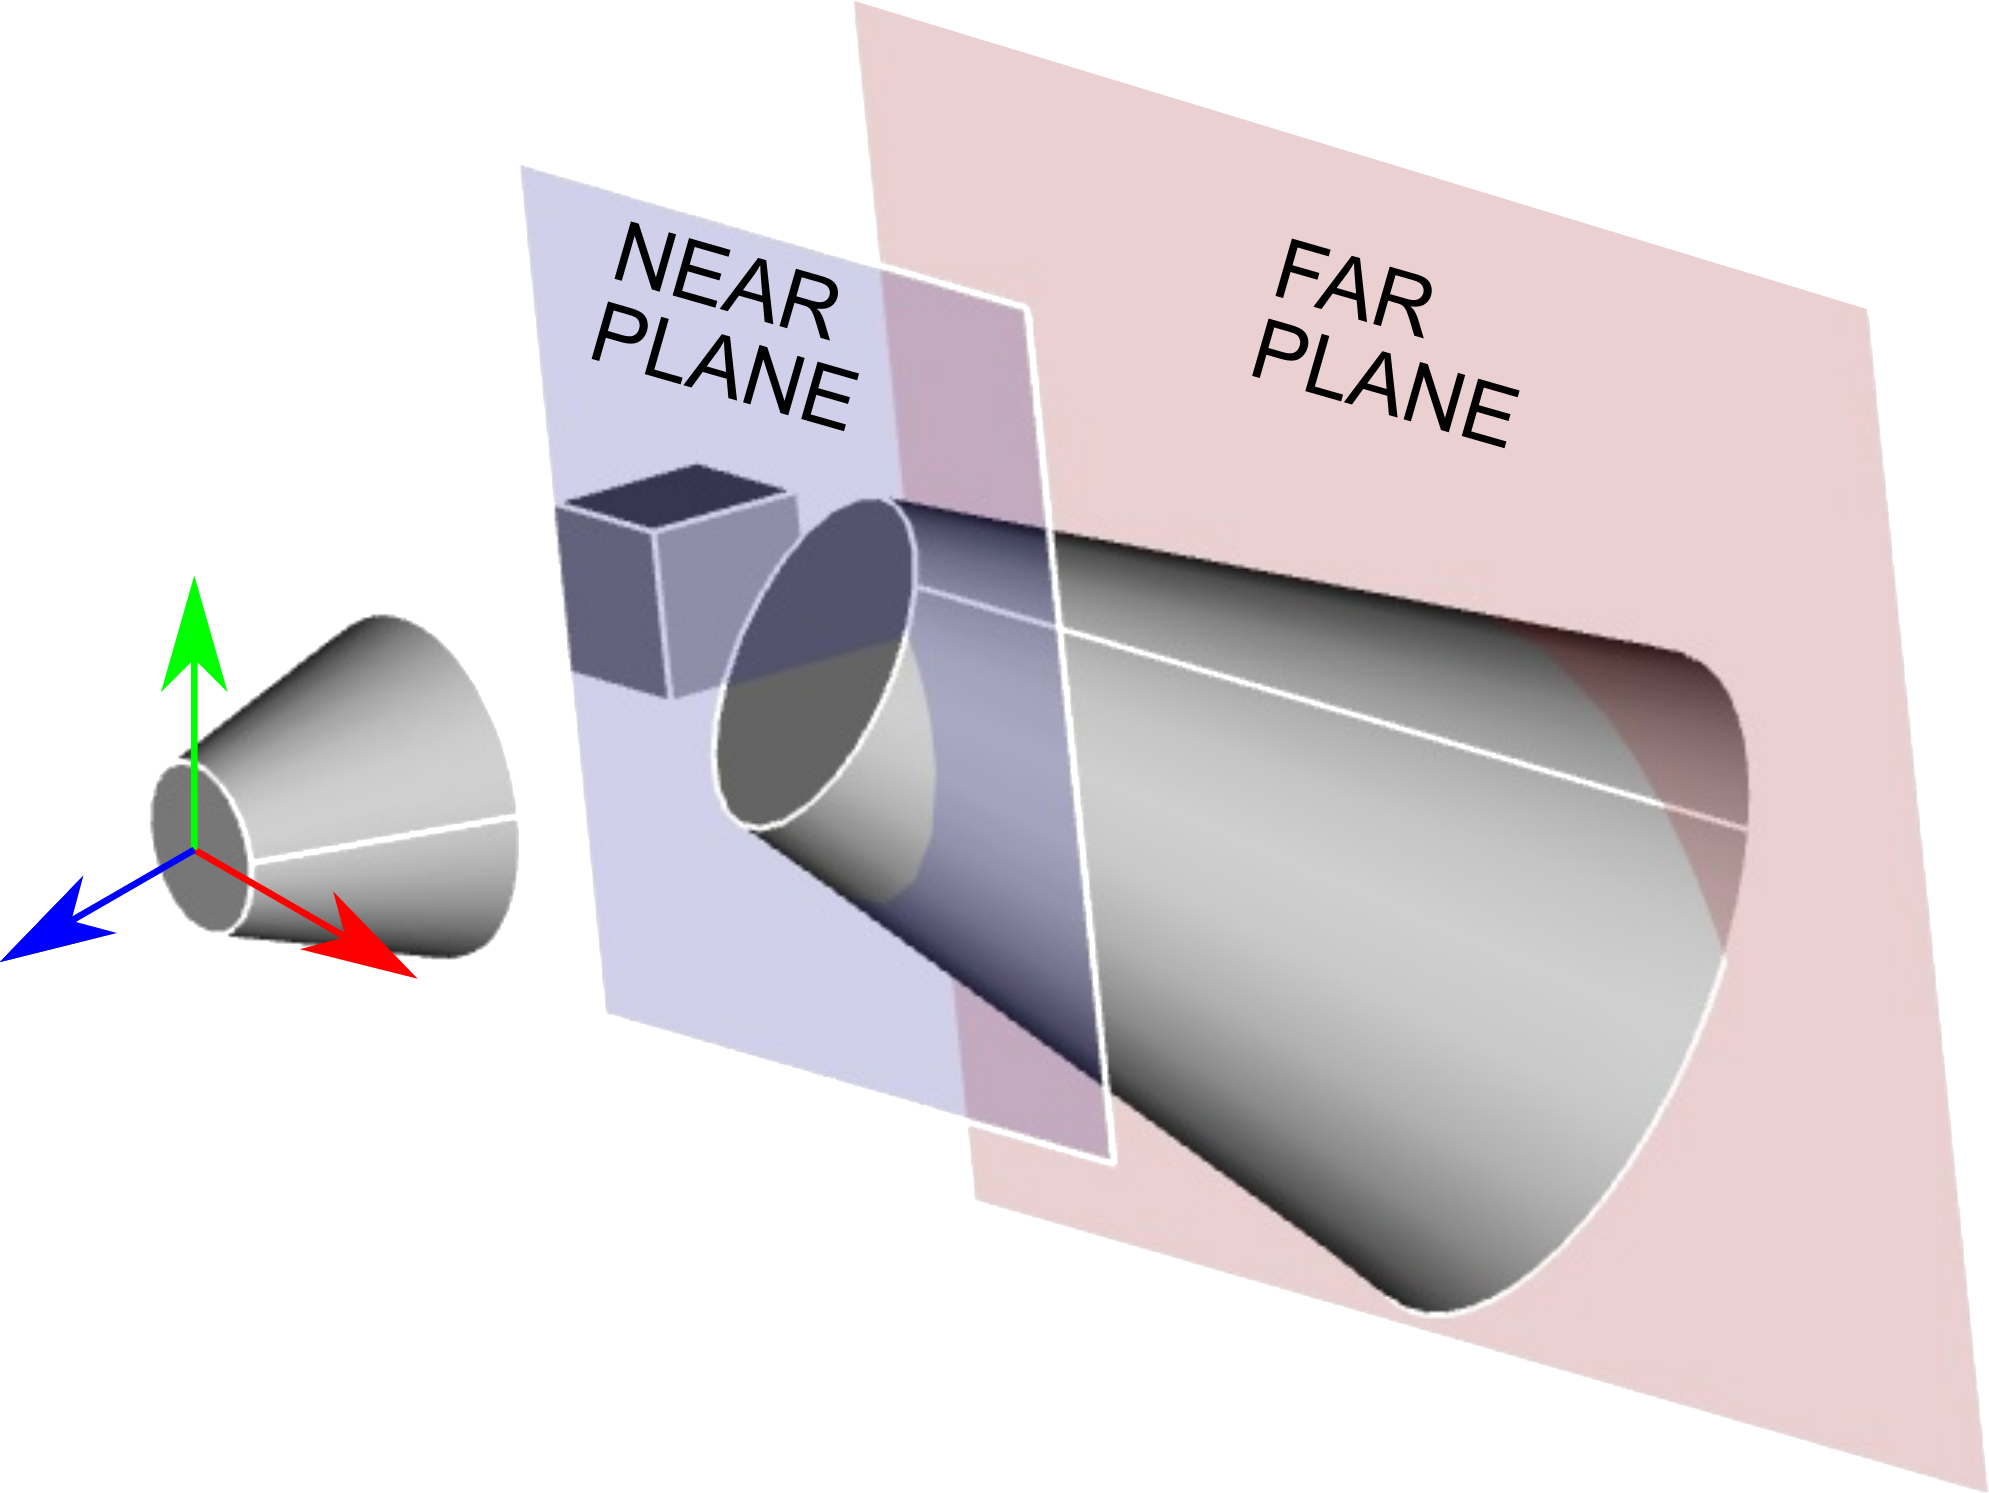
\includegraphics[width=4in]{./Graphics/clipping_planes}
  \caption{Defined into the camera's coordinate system (left), the near and far clipping planes are used to minimize the number of
  primitives to process, as well as reference points for depth computation. \label{fig:clipping-planes}}
\end{figure}

Raw colouring information in applied at this stage and primitives are finally
mapped into screen by a second $4\times 4$ matrix, the \emph{perspective
matrix}. At the end of this process objects are said to be in \emph{normalized
device coordinates \emph{NDC}}. In NDC, the (virtual) cube spawning the
$\left(-1,1\right)$ range in each direction is projected orthographically on the
output image buffer (considering $x$ and $y$ coordinates), with each corner
corrisponding to an angle of the window (called \emph{Viewport}) -- top, bottom,
right, left-- and depth buffer
(mapping the $(-1,1)$ $z$ coordinate to the range $\left( near , far \right)$ as described
before).

Finally, texture information in form of \emph{texels} (texture elements) is applied to primitives if needed and other
processing such as fog calculation is done. The image is completely rendered at
this point and can be accessed via direct reading from raw data buffers.

\subsection{Antialiasing of polygons and textures} \label{sec:antialiasing}
\label{sec:FBO}
%TODO antialiasing of textures
During the last phase of rendering, OpenGL's pipeline silently associate each
pixel primitive, with its matching texture and depth information, with a single
colour (RGB) and depth value (alpha). If only the geometric information relative
to the center of the pixels is considered (as done by default), this will cause
high rendering quality degradation: this is because contours of objects and
textures will be neatly mapped on a per-pixel basis, and so their lines --
especially if almost vertical or almost horizontal -- will appear more as a
polyline than a single, straight line. This effect is shown in fig.
\ref{fig:polyline}. To solve this issue, a set of techniques for what is called
\emph{antialiasing} are implemented. If implemented correctly, antialiasing of
polygons' edges and texture data can improve image quality by blending the
boundaries between adjacent polygons, thus providing a more photorealistic
render.

\begin{figure}[htbp]
  \centering
  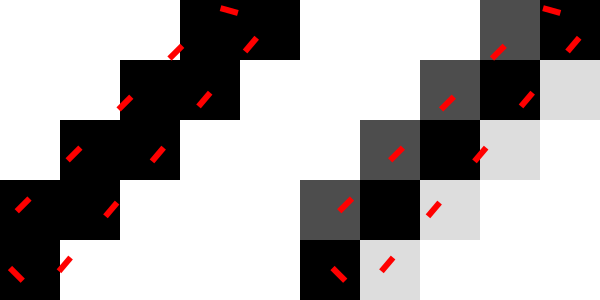
\includegraphics[width=2.5in]{./Graphics/antialiasing}
  \caption{A 1-pixel line generates rough boundaries on when rendering on a
  per-pixel basis. Multisample antialiasing can solve the problem by
approximating the line as a 4-pixel rectangle and averaging each multisampled
pixel with its neighbours. \label{fig:polyline}}
\end{figure}

Old versions of OpenGL provided a set of features called \emph{smoothing}, which
emulated transparency (alpha) value on pixels on the border in order to blend
them with neighbour pixels. Newer versions have deprecated this techniques in
place of \emph{Multisampling}. By using multisampling, each pixel primitive --
as the one obtained after the rasterization process -- is actually splitted in
four or more parts into a special, offscreen buffer, and the image is treated as
it was a render with higher resolution, except for coordinate systems which will
be left untouched -- so that the entire process is transparent to the
programmer. After rendering, the offscreen buffer is copied to the result buffer
and is said to be \emph{resolved}: in this stage, each pixel is formed by
averaging the content of the four micro-pixels which compose it. Multisampled
has been preferred over smoothing because, although requiring a lot of memory
for storing the high-resolution image -- which is not a problem with modern
graphics hardware as it was when smoothing was born --  it provides both faster
performance and better quality, as explained in \cite{opengl-book}.

The special buffer for offscreen rendering is implemented in OpenGL through the
means of a \emph{Framebuffer object (\emph{FBO})}.
Framebuffer objects are special drawing buffers, introduced with OpenGL 3.0,
which emulate a real framebuffer (i.e. the are of a video memory which
the software will draw onto), keeping the allocated memory area totally
independent from the actual video memory of the rendering window. Apart from
their physical location, they look totally equivalent to a normal rendering
window, and just like it they have a set of buffers to which the application can
draw, the main ones being the color and depth buffer. These can be bound 
at runtime to a physical location in memory by assigning (\emph{plugging}) new buffers to the \emph{attachment point} of a
framebuffer. A framebuffer can be drawn onto if and only if it is
\emph{complete}, i.e. if all its main attachment points (colour and depth) have
been bound to a physical buffer.

Apart from multiple uses which are irrelevant for this project (like dynamically
updating a texture by offscreen rendering onto it), the main scope of FBOs is
their multisample capabilities. In fact, it is sufficient to plug
multisample-capable buffers (which can be generated using OpenGL's allocation
functions) to the colour and depth attachment points of an FBO and select the
latter as the default rendering buffer to have the application draw all of its
raster data there, thus keeping multisample into account. 

When the final render has to be read, however, it is not sufficient to read the
raw drawing buffer from the FBO, as it has a totally different internal
structure in order to keep track of the needed geometric transformations needed
not to change the geometry's position despite of multisampling. A special
function, called \emph{blitting}, can be used to copy the multisampled data to
another framebuffer, allocated with raw RGB pixels and thus capable of being
read with the expected result. When blitting is applied to the multisampled
framebuffer, it is automatically resolved to pixels; in this way, the resolved
buffer can be copied byte-per-byte into the raw FBO.

Texture multisampling is also implemented with this method and provides a good
result. However, for textures the situation is different as also another factor
must be considered: as the object reduces
its dimensions, texture internal data will be dropped during the mapping from 3D
to 2D coordinate, because it actually is applied on a per-2D-pixel basis during the
last stage of rendering (after rasterization has been done), as depicted in sec.
\ref{sec:opengl-rendering}. This process downsamples heavily the texture -- even if
polygon multisampling is enabled -- as no interpolation is done when scaling
down the texture for appliance.

To solve this issue, OpenGL allows the programmer to specify a set of textures
of different size for the same object. Element of this set, which can be easily
generated automatically starting from the biggest texture, are called
\emph{mipmaps}. At the 2D texturing stage, OpenGL will choose the correct image
to map points to, and $(u,v)$ coordinates on it, based on a \emph{strategy}
which can be defined at runtime. Simpler strategies assume for example to always
take the first texture which is bigger or smaller than the primitive to cover,
while more complex ones allow to refine the result at expense of a bigger
computing time, by linearly interpolating between these two textures to produce
a middle texture component.

As said in sec. \ref{sec:opengl-intro}, OpenGL tends to be extrimely frugal in the
number of implemented features: the only supported method for adding mipmaps to
a texture is manually adding a series of differently sized images to the texture
data. As it is quite easy to generate this data automatically and with good
quality, however, the GLUT library exports useful functions to automatically
build the set of textures of increasing size and adding them to the texture.
A native extension for OpenGL allows to generate mipmaps when and only when
needed, at the cost of random loss of GPU cycles into the program; this extension is,
however, only present in newest versions of OpenGL and is not supported by some
graphic hardwares (e.g. Intel HD4000). The programmer must explicitely check for
its presence, and only when the extension is found by OpenGL he can safely
assume that no manual (or semi-automatic) mipmap generation is needed.

Texture mipmaps allow a 3D rendering application to reduce at its minimum the
number of discarded of data due to texture downsampling: instead, they allow to
produce high-quality, low-sized images when initializing the system (i.e. when
the program can afford to lose time to produce this data using complex filters
such as cubic interpolation). The visual result of texture mipmapping is
qualitative relevant and can be observed, together with the effect of
multisample on geometry, in fig. \ref{fig:multisampling-on}

\begin{figure}[htbp]
  \centering
  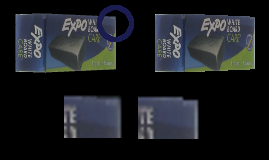
\includegraphics[width=2.5in]{./Results/antialiasing}
  \caption{Rendering with antialiasing and mipmapping on (left)
  can improve a lot the quality of the result with respect to the same options
turned off (right). \label{fig:multisampling-on}.}
\end{figure}

\section{Implementation of objects' rendering} \label{sec:renderer3d}
With the details explained in sec. \ref{sec:opengl-rendering} in mind, a mesh renderer has been implemented, capable of
reading objects' meshes from files as needed; together with meshes, it reads the full model of
camera with which training has to be done, and renders them in the required
pose, also extrapolating useful informations from the render which can be used
for training. All the interface of the renderer with the external world is done
using the conventions of the whole project: cameras are modelled using OpenCV's
standard reference systems and calibration matrices described into sec.
\ref{sec:camera_modelling}, while object poses are described as affine
transformations acting on homogeneous coordinates as in sec.
\ref{sec:homogeneous-coordinates}. At time of objects' creation, the Assimp library
is used to convert the mesh file, in whichever format it is, into Assimp's
unified structure, which for simplicity's sake can be simplifiethought of as a tree of
nodes, each representing a face, a texture to be applied to children, or
an affine transformation to be applied to children. When the renderer is created
it configures itself using GLUT to open a window and create the RGB and depth
framebuffers in which to render. Renderer's initialization is a one-time
operation, and is performed statically by the first object using GLUT. During
this phase, renderer also initializes the needed parameters for multisampling as
described in sec. \ref{sec:antialiasing}.

Three main features have been implemented, which can be used as an access point
to the renderer: the first one can set the
camera model by reading it from the project's camera data structure; the second
one can set the reference position of objects into camera's space (in this project's
conventions, i.e. in OpenCV not in OpenGL one); the third function can render a
mesh and extract RGB and depth buffers to OpenCV matrices for later use. This
last feature also extracts object's bounding box information and rendering mask,
which will be used for training and recognition filtering in sec.
\ref{sec:vision}.

\subsection{OpenGL camera modelling}
The goal of the first set of functions of the renderer is to interface OpenGL's
projection system with the global camera models used into the project; in
OpenGL camera's parameters are not defined and only a single matrix is used to
transform 3D coordinates in camera frame to 2D points onto the image. Keeping in
mind the definitions of intrinsic parameters of the camera, as described in sec.
\ref{sec:intrinsics}, this is accomplished into three steps.

First, the intrinsic matrix of the camera is extracted from the
camera's model, and from it the relevant camera parameters are read.

From this data, the projection matrix 
\begin{equation}
  M_{\text{int}}=\begin{pmatrix}
    f_x & 0 & -c_x & 0\\
    0 & f_y & -c_y & 0\\
    0 & 0 & (N+F) & NF \\
    0 & 0 & 0 & -1 
  \end{pmatrix}
\end{equation}

is built. This matrix is similar to the camera intrinsic matrix, but with two
main differences: first and most important, it operates on 3D points (in clip
coordinates) producing
other 3D points. If applied to a point, $x$ and $y$ coordinates in output are the same as they would be
if mapped using intrinsic matrix, but $z$ coordinate is mapped to the $near-far$
range. Second, the Z axis points forward in our convention, backward in OpenGL.
Thus the matrix is built so that the Z coordinate will be inverted while
preserving X and Y.

After this, clip coordinates have been transformed in what would are OpenCV's
camera coordinates, plus $z$. In order to port them into OpenGL's NDC, another
transformation is needed, which simply scales the view range (\emph{view
frustrum}) to linearly fit the NDC:

\begin{eqnarray}
  L = x_{\text{left}} & = & 0 \nonumber \\
  R = x_{\text{right}} & = & W_{\text{cam}} \nonumber \\
  B = y_{\text{bottom}} & = & H_{\text{cam}} \nonumber \\
  T = y_{\text{top}} & = & 0 \nonumber \\
  M_{\text{fit}} & = & 
  \begin{pmatrix}
    \frac{2}{R-L} & 0 & 0 & -\frac{R+L}{R-L} \\
    0 & \frac{2}{T-B} & 0 & -\frac{T+B}{T-B} \\
    0 & 0 & -\frac{2}{F-N} & -\frac{F+N}{F-N} \\
    0 & 0 & 0 & 1
  \end{pmatrix}
\end{eqnarray}

The two matrices are multiplied to get the final projection matrix, which is
passed to OpenGL as the matrix which maps clip coordinates to NDC:

\begin{equation}
  M_{\texttt{proj}}=M_{\text{fit}}M_{\text{int}}
\end{equation}

Also, OpenGL is instructed to which pixels and depth ranges correponds to the
NDC by setting its \emph{viewport}, \emph{near} and \emph{far} values.

At the end of this process, OpenGL will thus map automatically points in global
3D space with points in camera frame.

\subsection{Object movement into global space}
Into the project's convention, each object has got its own local coordinate
system, and the mesh is built with all its verteces into this system,with all
its verteces into this system,  as explained into sec. \ref{sec:cad-mesh}. Every
object is then stored into its mesh file as if it was centered into the global
origin. Assimp library is used to read this mesh file and produce a set of faces
together with their vertices' coordinates. From the external world, however, the global
renderer can display a mesh into a specified pose in the global coordinate
system obeying the specifications of the project. This system is different from
OpenGL's one, which only knows camera (clip) coordinates. In order to move
the object from the global system to the right position in OpenGL reference
system the \emph{Modelview} matrix is used: this will be automatically applied
to OpenGL when drawing each primitive, and will modify its coordinates
accordignly. In order to take into account the difference between the global
coordinate system and OpenGL's clipping coordinates, a $\pi$ rotation along the
$X$ axis is applied
to the Modelview matrix \emph{before} the actual pose, which as usual is
already represented as a $4 \times 4$ affine transformation matrix:

\begin{equation} \label{eqn:modelview}
  M_{\text{modelview}} = 
  \begin{pmatrix}
    1 & 0 & 0 & 0 \\
    0 & -1 & 0 & 0 \\
    0 & 0 & -1 & 0 \\
    0 & 0 & 0 & 1 
  \end{pmatrix} M_{\text{pose}}
\end{equation}

Another convenience function is presented to the user, which can emulate
camera's movement around the object: in this case, the object's pose is first
computed as the inverse of camera pose ($M_{pose}=M_{cam}^{-1}$), and it is
finally applied as in eqn. \ref{eqn:modelview}.

\subsection{Object rendering and image processing} \label{sec:meshdraw}
When all the rendering parameters has been set accordingly to the desired scene
parameters and emulated camera model, the renderer can be asked for to finally
get the rendered image of a mesh object. When done, it is actually the mesh that
renders itself into the OpenGL's framebuffer. As the mesh knows its internal
data as a tree structure, a recursive rendering algorithm is applied. Starting
from the mesh's root node:

\begin{itemize}
  \item{If the node contains a transformation, this has to be applied to the
      current node and all his children. Thus, the transformation matrix data is
      extracted from the node and it multiplies the current Modelview matrix.
      The old value of the Modelview matrix is saved in a stack using OpenGL's
      builtin facilities, in order to be restored when this node will end its
    drawing;}
  \item{If the node contains one or more meshes (here, indicating a set of
      faces sharing a common texture), these are drown into the scene: first the
      appropriate texture is loaded, then each face is drown considering its
      number of vertices $N_v$: either as a point (if $N_v=1$), or as a line (if
    $N_v=2$), or as a polygon (if $N_v \geq 3$);}
  \item{If a texture must be applied to the previously drown face, or the face
      has solid colour, it is applied at this stage. In the case of a 2D
    texture, UV mapping information is mapped to the vertices of the face;}
  \item{If the node has children, these are drown recursively. When the children
      start drawing themselves, the Modelview matrix will correspond to the
      stacked transformation of their parents: in this way, they will be able to
    specify their vertices' data in their local coordinate system;}
  \item{Finally, the previously stored Modelview matrix is popped from the stack
      in order to restore the initial state for the following nodes. The
      control is returned to the caller, be it its parent or the
    original caller of the drawing algorithm.}
\end{itemize}

When the algorithm exits, thus, the mesh will be drown on OpenGL's FBO %TODO
%capitoletto su FBO 
with both colour and depth informations and the render is ready to be read from the
caller's process. Also, the final state of OpenGL's render is equal to the
starting one, which allows to draw more than one mesh singularly without
setting the parameters for each.

\subsection{Framebuffer's data acquisition}
As all data has to be rendered off-window, OpenGL's \emph{framebuffer objects
(\emph{FBO})} have been used as explained in sec. \ref{sec:FBO}. Two main FBOs
are generated and replaced each time the camera model changes its dimensions:

\begin{itemize}
  \item{The \emph{Multisampled FBO} is the FBO that the application will
      actually use when drawing. At the time of its creation, two buffers are
      created, both of which with multisample capabilities of $4\times$. The two
      buffers are then bound to the attachment points of the FBO, one for colour
    and one for depth information;}
  \item{The \emph{Resolve FBO} is the FBO on which the previous FBO will resolve
      itself by means of blitting: it has two buffers like the previous one, but
      these are raw, non-multisampled buffers. These are actually internally
      represented as a C matrix and can thus be read sequentially.
      When the user wants to read the render's result, the multisampled FBO is bound
      as the FBO from which data have to be read, and the resolve FBO is bound
      as the FBO on which data have to be drown. The blitting function will copy
      the viewport area of the render and automatically resolve the
      multisampling. The resolve FBO is finally bound as the default FBO. The
      caller process can then read raw data from the default FBO and get
    back the multisampled render result in RGB format.}
\end{itemize}

When an application wants to drive something into the rendering, it first binds
the drawing buffer to the multisampled FBO, then calls its drawing algorithm as
explained in sec. \ref{sec:meshdraw}. Finally, it resolves the FBO as above and
reads the pixels' data from it. In order to comply with the global, internal
specifications of the project, this data is transformed into a \texttt{cv::Mat}
object; no data copying is needed because OpenCV's matrices' internal format is
the same as raw C buffers and camera frames have been set accordingly to both
specifications to have the result fit.

\subsection{Render postprocessing}
At the end of the rendering process, the renderer performs a simple serie of
operations which will be needed in the later training and recognizing process:

\begin{itemize}
  \item{
    First, the real depth values are reconstructed from the 12-bit value
    provided by OpenGL. These will be useful for normal feature estimation by
  the training algorithm;}
  \item{then, an object mask is generated for the render. This is intended to inform
the caller on which pixels on the image correspond to the actual object and
which are simply background. In order to find it, each depth value is checked to
be comprehended in the $near,far$ range which was set into OpenGL: if it isn't,
this means that the pixel was not generated by the render (it is 0 or NaN, i.e.
the depth buffer's clearing value);}
  \item{next, the object's bounding box is extracted from the mask. Assuming it
to be a rectangle, the bounding box can be computed by considering the minimum
and maximum $u$ and $v$ values in which the mask is not null:
\[
  \begin{array}{c}
    m_u=min\left(\left\{u | \exists i, mask_{(u,i)}\neq 0\right\}\right),
    m_v=min\left(\left\{v | \exists i, mask_{(i,v)}\neq 0\right\}\right) \\
    M_u=max\left(\left\{u | \exists i, mask_{(u,i)}\neq 0\right\}\right),
    M_v=max\left(\left\{v | \exists i, mask_{(i,v)}\neq 0\right\}\right) \\
    \Downarrow \\
    \text{rect}=\left\{\text{rectangle of width } M_u-m_u \text{ and height } M_v-m_v
    \text{ starting from } (m_u,m_v)\right\}
  \end{array}
\]
}
\item{finally, the RGB image is cropped to the rectangle found in the previous
    step. This will allow faster feature computation, possibility to easily save
    frames, low memory bandwidth usage (which is not negligible as the rendering
  process will be done thousands of times).}
\end{itemize}

The renderer returns all of this information to the caller, who will be able to
use it for image processing.

\section{Offline template generation using 3D meshes and OpenGL} \label{sec:training}
In order to efficiently train the object database for each model, it is needed
to create a big set of templates, which is able to cover the whole set of view
points. Training can be performed with either \emph{online} methods (i.e.
Physically looking at the object from different viewpoints with the chosen
camera) or \emph{offline} ones, which build the dataset starting from known
object informations such as pre-extracted colour features or shape informations.

In this section we present the proposed method for template database
creation, which is an implementation of the method used by modern template
matching algorithms such as \cite{linemod-paper} and \cite{TODO}, and
has the advantage of being quite fast, fully automated for any dataset size,
and highly scalable (different datasets from different vendors can be merged
together or distributed with no effort at all).

\subsection{Offline training advantages}
It has been suggested in \cite{TODO} that fully-automated, offline training method can
outperform online training methods used as a de-facto standard
in previous years \cite{TODO}. Main advantages of offline training methods like
the proposed one, with respect
to online ones, include:

\begin{itemize}
  \item{Offline training does not require human intervention. Human-based
      training is error prone, and cannot yield to good results if not done by an
      \emph{expert} person. In an industrial or research scenario, this implies
      employing a skilled human resource in a non-productive task, which has obvious
      consequences in terms of costs (at least if the process is repeated
      for a big group of objects) and team productivity (the charged person will be
      actually involved full-time in a task which is well below is actual
    capabilities);}
  \item{Accurate training is a time-consuming task and physical objects must be available. In an
      industrial scenario, this can mean a longer time-to-market or delayed custom products deli-
      very. On the other hand, offline training does not require a physical copy of the object: for
      example, the proposed approach only needs a CAD model of the object, which in modern
      scenarios is available well before the final product; this means that training can be done at
      early project phases, before the objects used for testing the project actually
    arrive;}
  \item{If offline training is accurate enough, it can bring much more precise results than online
      one. For example, pose information associated with each template are exact when generated
    offline, while naturally prone to human error if estimated online;}
  \item{Large objects can be modelled without the need of physical movement around them. As
      algorithms such as \cite{linemod-pipeline} will probably evolve their already good real-time capabilities, they will
      be able to be applied to environments such as cities, in which the traceable objects are too
    big to be modelled online at low cost.}
\end{itemize}

\subsection{CAD modelling of objects} \label{sec:cad-mesh}
The idea behind the training procedure is to exploit CAD models of the object
to recognize in order to generate realistic renders of it and use the latter
for feature extraction and database training. In this way, a physical camera is
simulated and full viewpoints' coverage can be easily obtained.

For the purpose of the thesis, meshes have been built with Blender
\footnote{www.blender.org} and FreeCAD \footnote{www.freecad.org}. The first is a
well-established free (GPL) software for 3D graphics, while the second is an
emerging free (LGPL) general-purpose CAD application. After modelling each
object with the CAD capabilities of FreeCAD, the corresponding mesh has been
exported using a common file interchange format (\texttt{.obj}) and has been
textured in blender by using photos of the object taken with a digital camera,
exploiting Blender's advanced UV unwrapping and mapping capabilities. The result
is a realistic model of the object like the one shown in fig.
\ref{fig:realistic_rendering}, correctly textured to mimic the real one.

\begin{figure}[htbp]
\centering
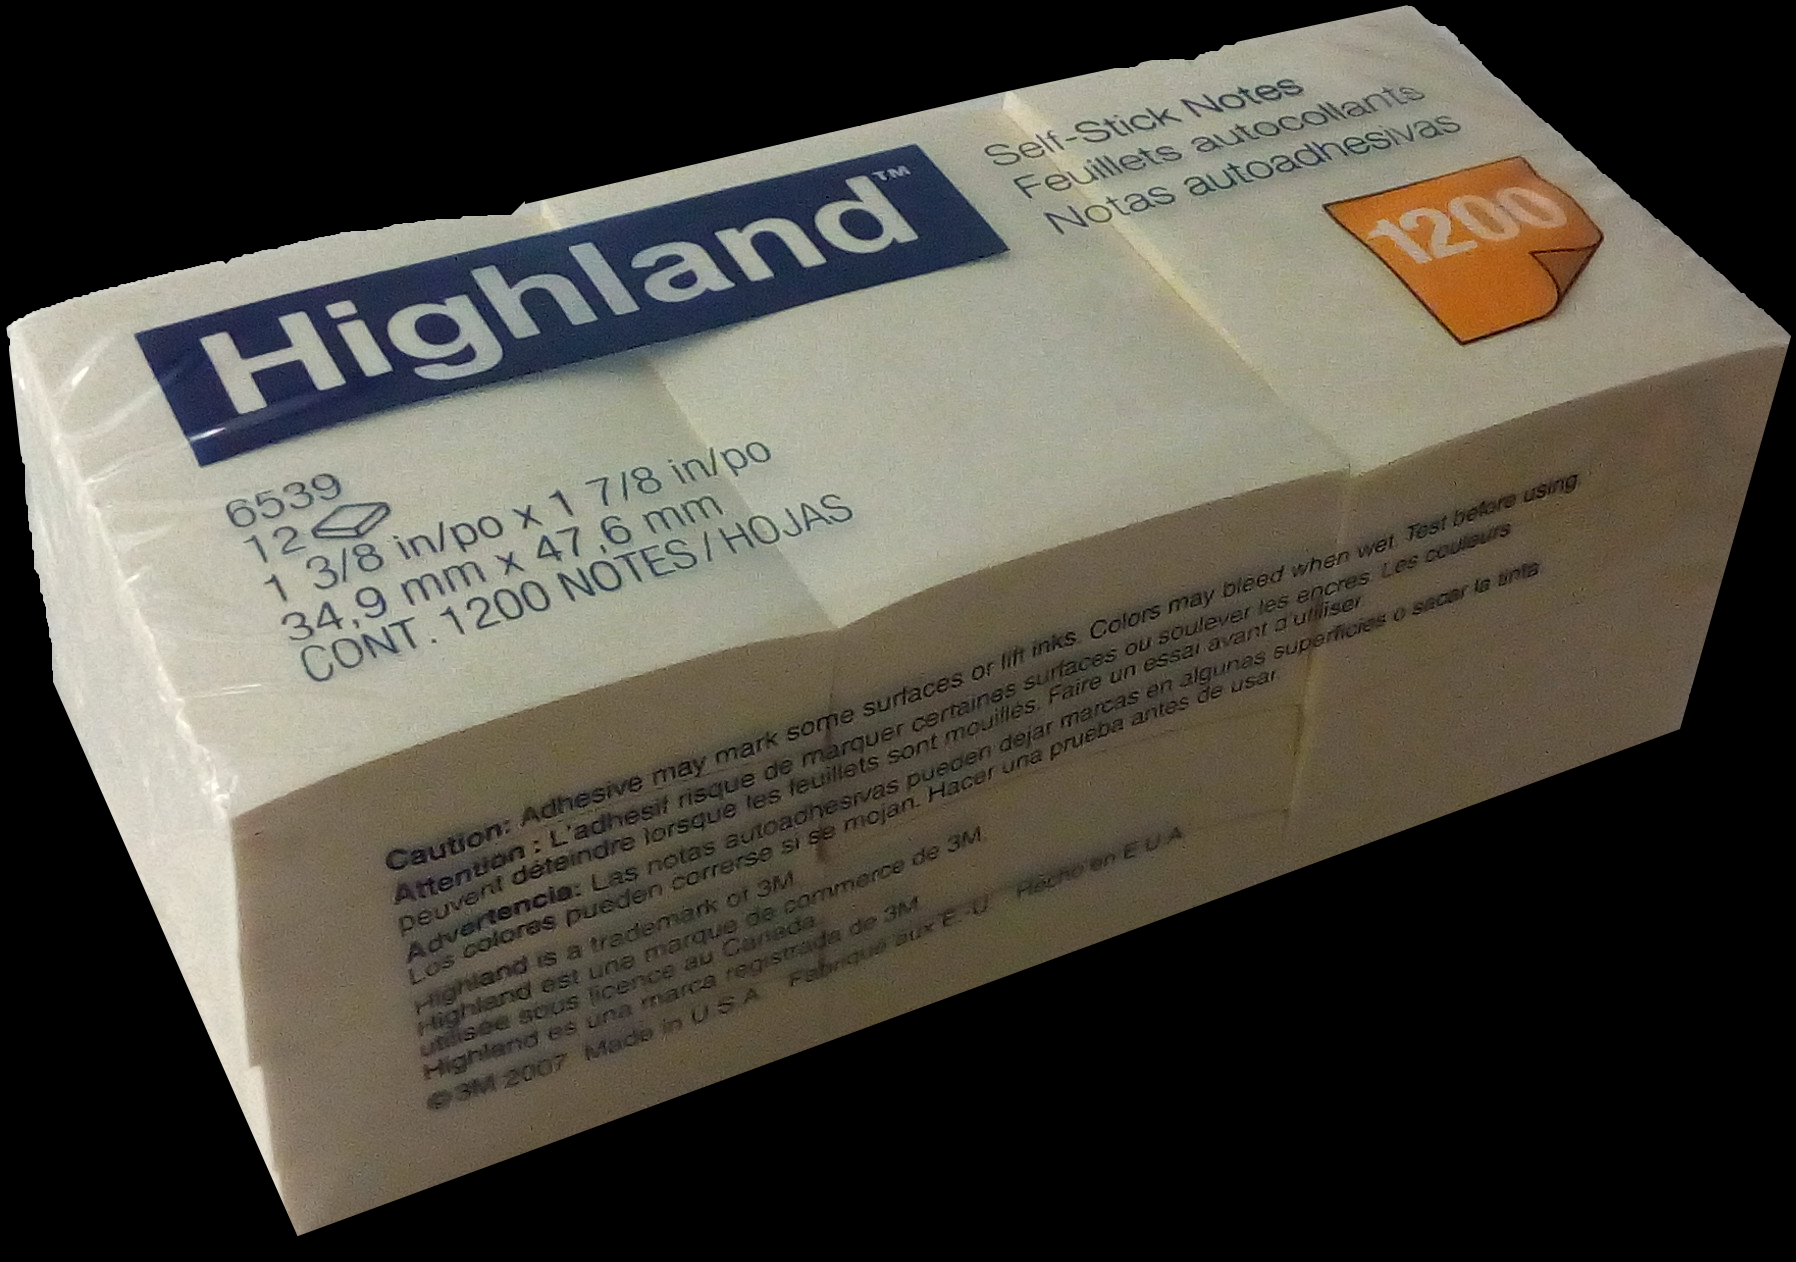
\includegraphics[height=1.5in]{./Results/postit_photo}
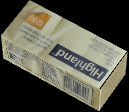
\includegraphics[height=1.5in]{./Results/postit_render}
\caption{Example rendering of mesh: the rendered mesh (right) is photo realistic
  if compared to real images (left),
and thus adequate to be used for template generation. \label{fig:realistic_rendering}}
\end{figure}

\subsection{Enumeration of possible object's positions}
The problem of covering the whole viewpoints' set for a particular object
implies a tight compromise between training speed, execution speed and
reliability. In fact, the number of templates needed for a particular object increases
both training time and recognition time. However, as the training procedure is
fully automated and not very long (about 15 minutes per object, as depicted in sec.
\ref{sec:TODO}), %TODO results-time cite check
the running time of the recognition algorithm is the main problem if too much
templates are generated. On the other side, if the object is not trained enough
at different positions and values, it could be not recognized correctly and the
whole algorithm could then fail.

The first discriminant to ensure running time is not wasted is not having
redundancy when enumerating possible poses: this excludes enumerating them via
increasing Euler Angles, as they can generate redundant transformations.

The chosen solution is to virtually keep the object still in the origin and
moving the camera around it, on the surface of a sphere of increasing radius.
This allows to enumerate all the rotations once, and at different distances too.

Two main methods exist to generate points on a sphere, which are the same
used by mainstream 3D graphics tools for mesh generation: U-V coordinates (i.e.
increasing latitudes and longitudes), and icosahedron cutting (the result of
which is called \emph{icosphere}). 

As depicted in fig. \ref{fig:uvsphere_vs_icosphere}, generating a sphere by changing latitude and longitudes of points has the 
disadvantage of having different points' densities between the poles and at the
equator, as changing longitudes results in a smaller movement if latitude is
near poles. 

The second -- and chosen -- method consists of starting approximating the sphere
as a convex icosahedron, and then iteratively subdividing each face in four
smaller faces, keeping the same radius in order to better approximate the sphere
itself. It can be easily seen that this is the best method to provide uniform
sampling method on the whole surface of the sphere, as each point will always be
at the same distance from its neighbours. 

\begin{figure}[htbp]
\centering
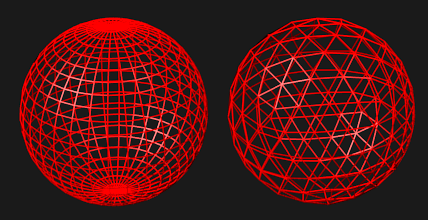
\includegraphics[width=4in]{./Graphics/uvsphere_vs_icosphere}
\caption{UV sphere (left) and icosphere (right): the latter has uniform distance
between points, which is a desirable property. \label{fig:uvsphere_vs_icosphere}}
\end{figure}

After subdividing the sphere and reaching the minimum required number of points,
the camera is moved onto each point and rotated in-plane, in order to complete
the enumeration of poses. The whole process is repeated at small distance steps
($5\sim10\unit{cm}$), so that the object can be recognized at different positions too.

After generating camera's position, its rotation is generated by computing the
camera's $\vec{up}$ vector (as defined by OpenGL \cite{opengl-book}) as a linear
combination of the vector perpendicular to the point's vector, heading to the
north pole, and the vector perpendicular to the point's vector, with horizontal
direction, heading east:

\begin{equation}
  \begin{array}{ccc}
  \vec{h} & = & \frac{ p  \times \vec{Z}}{\left\lVert p  \times \vec{Z}
  \right\rVert} \\
  \vec{v} & = & \frac{ p  \times \vec{Y}}{\left\lVert p  \times \vec{Y}
  \right\rVert} \\
  \alpha_i & = & \frac{2\pi}{i_{max}} i \\
  \vec{up}_i & = & \vec{h} \sin(\alpha_i) + \vec{v} \cos (\alpha_i)
  \end{array}
\end{equation}

Knowing camera's position $\vec{P_c}$ and $\vec{up}$ vector, the transformation matrix of
the camera with respect to origin can be computed as done in OpenGL:

\begin{equation}
  \begin{array}{ccc}
  \vec{f} & = & -\vec{P_c} \\
  \vec{s} & = & \vec{f} \times \vec{up} \\ 
  \vec{u} & = & \left( \frac{\vec{s} }{\left\lVert \vec{s}\right\rVert} 
  \right) \times \vec{f} \\
  M & = & \left(
  \begin{array}{cc}
    s & -x_c \\
    u & -y_c \\
    -f & -z_c  \\
    \vec{0} & 1
  \end{array} 
  \right) \\
  \end{array}
\end{equation}

\begin{figure}[htbp]
\centering
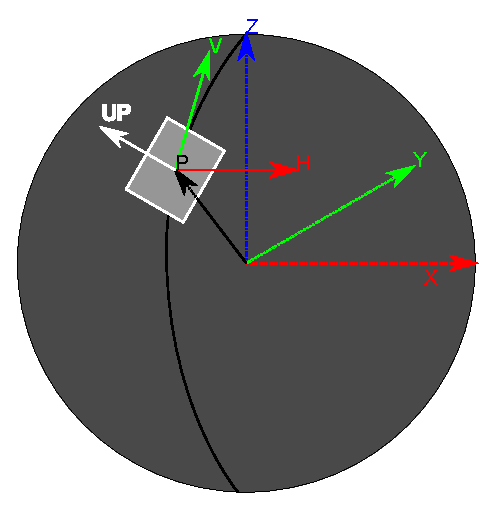
\includegraphics[width=3in]{./Graphics/up_vector}
\caption{In-plane rotation of camera by generating $\vec{up}$ vector as a linear
combination of plane's direction vectors \label{fig:up_vector}}
\end{figure}

This matrix is finally inverted to transform it in the object's position
relative to the camera, as it is in the coordinate system of the latter that the
object's pose will be estimated.

The object is then rendered on RGBD images into its position using the OpenGL renderer
described in sec. \ref{sec:opengl-rendering}. The rendered RGBD image, together
with the object's mask generated from rendering, is finally passed to the chosen
detector in order to extract a template.

\section{Line-MOD template matching} \label{sec:linemod}
Template matching has always been an attractive approach to computer vision,
especially for real-time applications; some of the main reasons for this
include ease of generalization of
these algorithms (several shapes can be associated to the same object), and
variety of applications (from rigid object detection -- like in this project --
to face recognition); another great advantage over other recognition methods,
such as neural networks, is the need of a relatively simple and fast training phase:
statistics-based methods, in turn, usually require a huge amount 
of samples to be given for evaluation. Usage of template matching also opens
the possibility of starting with a small, offline-generated template database, and training the
objects to be recognized \emph{online}, i.e. acquiring new samples while
recognizing them. In this sense, template matching offers both the benefits of
a fast, model-based training stage and the benefits deriving from
machine-learning algorithms, improving their performance the more they operate.

Two usual problems often come with template-based solutions: the first is that,
as a template usually consists of a set of features to be searched into the
target image, the high-number of templates (even for a relatively small
database) makes this technique come with an extremely high computational cost;
on the other hand, statistical methods require a much longer training phase but
usually base themselves, at recognition time, on a well-defined, very small set of
data (e.g. hue histograms, network coefficients) which is not proportional to the number of elements
analysed during training phase. Also, template matching usually has poor
results when the analysed object has little texturing information, as a low
number of features (\emph{keypoints}) can be extracted for each datum.

The Line-MOD template matching algorithm was introduced in 2011 by
Hinterstoi{\ss}er, S. et al. (\cite{linemod-paper}) as a way to address these
two problems of template matching approaches. It is based on a previous work by
the same authors, \cite{linemod-origins}, in which the LINE algorithm was
descript, which solved both the problem of template matching velocity and
texture-less detection, modified to give increased robustness and detection
rates. Another, following work is described in details in sec.~\ref{sec:linemod-pipeline}, and focuses on a practical application of these
algorithms, which is the one to which the system proposed into this project has
inspired.

In this section, this algorithm is explained in detail. Its key concepts are
introduced first, such the concept of image gradient (sec.~\ref{sec:linemod-gradient}) and depth normal computation (sec.~\ref{sec:linemod-depth}). Then, the modality of data representation, which is
the main reason for this algorithm's good performance, is shown in sec.~\ref{sec:linemod-binary}, and finally the algorithm's operating principle is
detailed in sec.~\ref{sec:linemod-usage}.

\subsection{Gradient orientation of images} \label{sec:linemod-gradient}
In order to efficiently detect matches into a non-textured image, which is one
of the problems which Line-MOD proposes to solve, a good metric that can be
used for defining salient features into the image is the value (and direction)
of the image \emph{gradient} $\vec{\nabla} (u,v)$ for each pixel. This vector
quantity is defined just like the discrete gradient for a function on the
domain $N$ of natural numbers: by quantizing the differential operator, the
discrete derivative of a function $f(x)$ is given by

\begin{equation}
\frac{df(x)}{dx}=f(x+1)-f(x)
\end{equation}

At the same way, an image can be seen as a set of  functions (one for each
channel) of two variables $(u,v)$, returning the corresponding pixel value at
the desired coordinate, for the desired channel. Thus, a partial, discrete
derivative can be computed onto this function, and the gradient can be defined
as usual as the vector of partial derivatives:

\begin{eqnarray}
\frac{\partial f(u,v)}{\partial u} & = & f(u+1,v)-f(u,v) \\
\frac{\partial f(u,v)}{\partial v} & = & f(u,v+1)-f(u,v) \\
\nabla f(u,v) = \begin{pmatrix} \frac{\partial f(u,v)}{\partial u} \\
\frac{\partial f(u,v)}{\partial v} \end{pmatrix} & = &
\begin{pmatrix}f(u+1,v)\\ f(u,v+1)\end{pmatrix}-\begin{pmatrix}f(u,v) \\
f(u,v)\end{pmatrix}
\end{eqnarray}

This is, anyway, an informal definition, which nevertheless finds its
application being simple to implement and computationally cheap. More formal
definitions exist, such the \emph{Sobel operator}, which instead of scanning the
image for difference into a single direction linearly approximates the image as
a continuous function -- it assumes, in fact, that the underlying intensity
function for each channel is continuous
and sampled only in correspondence of pixels' coordinates -- , and thus makes
uses of a convolution operator to approximate samples of the continuous
gradient $G(f)$:

\begin{eqnarray}
  G_x(f) &=& \begin{pmatrix} 
      -1 & 0 & 1 \\
      -2 & 0 & 2 \\
      -1 & 0 & 1 \end{pmatrix}
  \ast f \\
  G\_y(f) &=& \begin{pmatrix} 
      -1 & -2 & -1 \\
      0 & 0 & 0 \\
      1 & 2 & 1 \end{pmatrix}
  \ast f  \\
  G(f) & = & \begin{pmatrix} G_x \\ G_y \end{pmatrix}
\end{eqnarray}

Here, the $\ast$ operator represents convolution of a $3\times 3$ matrix $K$, called
\emph{kernel}, with another matrix $A$: after extending $A$ with a row of $0$ on
each of its four sides, the value of $K\ast A$ is defined for each coordinate
$(u,v)$ as:
\begin{equation}
  (K \ast A)_{u,v} = \text{sum}\begin{pmatrix}
    K_{0,0}A_{u-1,v-1} & 
    K_{0,1}A_{u,v-1} & 
    K_{0,2}A_{u+1,v-1} \\ 
    K_{1,0}A_{u-1,v} & 
    K_{1,1}A_{u,v} & 
    K_{1,2}A_{u+1,v} \\ 
    K_{2,0}A_{u-1,v+1} & 
    K_{2,1}A_{u,v+1} & 
    K_{2,2}A_{u+1,v+1}  
  \end{pmatrix}
\end{equation}

Depending on how the gradient of the image is approximated, the result could
slightly change. However, the intuitive concept is always the same. As an
example, the result of the application of Sobel operator $G$ on a reference
image\footnote{Image taken from the USC SIPI database
  ( http://sipi.usc.edu/database/ ), one of the most common computer vision reference
databases. Original source is unknown.}
 is shown in fig.~\ref{fig:scimmia}.

\begin{figure}[htbp]
\centering
\begin{tabular}{c|c}
  \multicolumn{2}{c}{\adjustbox{valign=m}{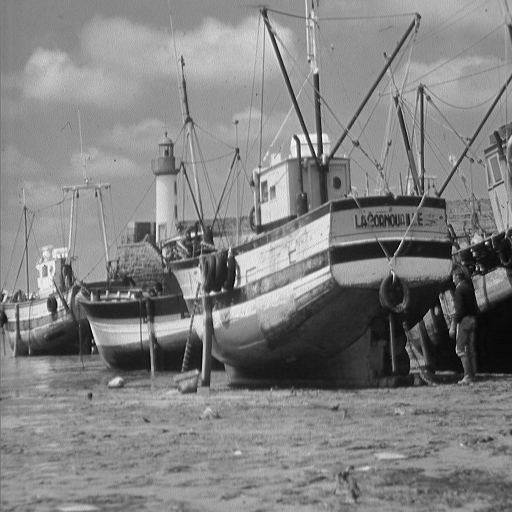
\includegraphics[height=2in]{./Graphics/scimmia}}} \\
    \multicolumn{2}{c}{\vspace{0.2in}} \\
  \adjustbox{valign=m}{
\includegraphics[height=2in]{./Graphics/scimmiagradient}} &
  \adjustbox{valign=m}{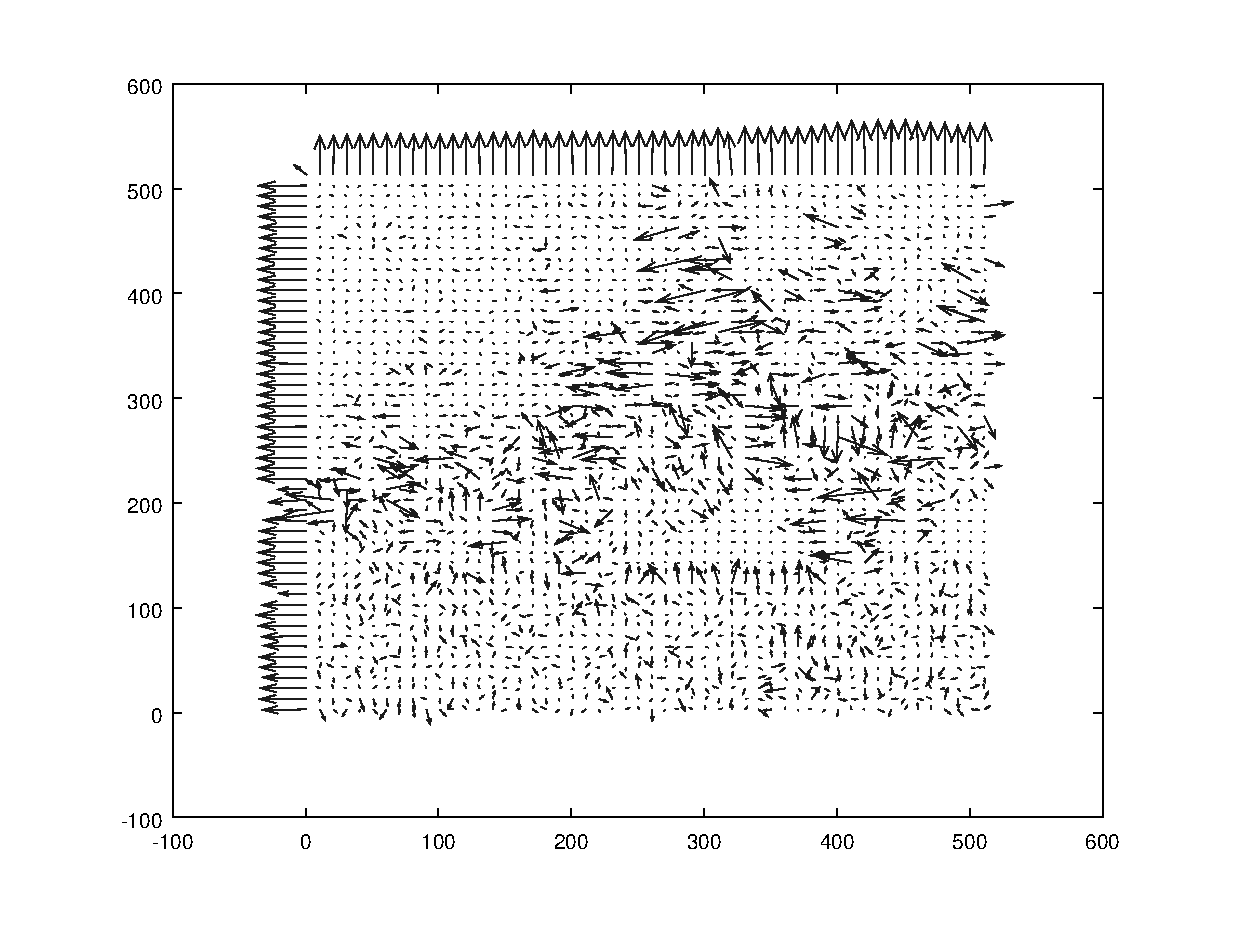
\includegraphics[height=2.5in]{./Graphics/scimmiafrecce}}
\end{tabular}
\caption{Grayscale, single-channel image (top) on which the Sobel operator $G$
has been applied. Resulting absolute value (left) and vector field
(right).\label{fig:scimmia}}
\end{figure}

\subsection{Fast normal computation from depth images} \label{sec:linemod-depth}
One of the most important features which can be extracted from a 3D
image is points' normals. These, just like an image's gradient, form a
vector field inside the image, representing the approximated normals
to the surface for which the RGBD picture has been taken, sampled in
correspondence of the image's pixel centres.

Of course, starting with sampled (and noisy) data from the image
implies that the normals which are computed are only a supposition:
if it is assumed that the quantized depth value is sufficient to give
informations about normals, the assumption must also be made that the
function is almost flat in local neighbourhoods, otherwise the Nyquist
theorem would be violated. With this assumption, nevertheless, it is
possible to approximate the planar surface corresponding to each pixel
with a plane connecting the plane and each of its neighbour points,
and from this compute the normal vector to each point.

The Line-MOD algorithm in its original implementation
(\cite{linemod-paper}) makes use of this idea to compute normals which will be used
as a feature for templates.

First, for each point $p$ in the image, the neighbour pixels are
considered. Assuming that the objects to be computed could be into a
cluttered scene, however, before taking each of them, a check is done
for drastic changes in the depth value $d$: if the variation is too
high (over a certain threshold $t_d$), this means that two separate
surface are actually considered, and this would break the assumptions
stated before, so the pixel is discarded; this technique also removes
possible outliers caused by bad sensor's performance.  The remaining pixels are put
into a neighbourhood set $N_p$. 

Considering the hypothetical plane which $p$ belongs to, its
orientation can be described by means of the gradient $\nabla$ of the
depth function $D(u,v)$. This, in turn, can be approximated by using first-order
Taylor expansion over the $(u,v)$ coordinate. For every point $p_2 \in N_p$:

\begin{eqnarray}
  p_2 & = & \begin{pmatrix} u_2 \\ v_2 
  \end{pmatrix} \\
  D(p_2)-D(p) & = & dp^{\tau}\nabla D (p) + o (p) \text{(Taylor
    expansion)} \label{eqn:taylor-depth-expansion}\\
  \nabla d(u,v) \approx \begin{pmatrix} \frac{\partial d(u,v)}{\partial u}
    \\ \frac{\partial d(u,v)}{\partial v}
  \end{pmatrix} & = & \begin{pmatrix} \frac{d(u2,v2)-d(u,v)}{u2-u} \\
    \frac{d(u2,v2)-d(u,v)}{v2-v} 
  \end{pmatrix}
\end{eqnarray}

With this approximation, each of the points in $N_p$ defines a
constraint over $N_p$, which is defined with the reasonable assumption
that at least 2 points in the neighbourhood will be considered
(otherwise, a null normal vector will be assigned to $p$). In the best
case of 8 valid neighbours, each of them is considered and, being the
system over-constrained, the
gradient $\nabla$ is computed in order to minimize the least-squared
error on eqn.\ref{eqn:taylor-depth-expansion}. This will smooth away
the noise on depth due to sensor's limitations and values'
quantization (assuming it is randomly distributed).

After computing the best approximation for the depth function's
gradient over $p$, the normal vector $N(p)$ can be approximated by computing
two principal axes of the surface's plane and deriving it from the
external product of these two:

\begin{eqnarray}
  dU & = & D(p)+\frac{\partial D(p)}{\partial u} \\
  dV & = & D(p)+\frac{\partial D(p)}{\partial v} \\
  N(p) & = & \frac{dU \times dV}{\lVert dU \times dV \rVert}
\end{eqnarray}
This algorithm, which is similar to what is implemented by most 3D
processing libraries -- most notably, Point Cloud Library --, produces
a good result in terms of an acceptable precision and a very good
performance. In this case, the latter is much more important as
precision in normal computation will be not very relevant, as the
algorithm will highly cut down the resolution of this computation to
better stand small transformations as explained in
sec.~\ref{sec:linemod-quantization}. On the other hand, computational speed
is important as Line-MOD wants to be able to have future real-time applications.

\subsection{Gradient and depth quantization} \label{sec:linemod-quantization}
The main innovation introduced by \cite{linemod-origins}, and thus by
\cite{linemod-paper}, is a big improvement over matching time due to
a novel, binary representation for templates' data. This
representation provides both fast matching time and robustness to small
deformation of the objects (or pose changes with respect to the
template's ground pose), as it spreads every feature into its surrounding
area, thus making it possible to detect them even in the case in which
they perform a relative movement between each other.

Before coding each template data with a binary pattern, it is
\emph{quantized}. The number of quantization steps to be considered
will affect many aspects of the algorithm's behaviour; in particular,
an high number of steps will result in bigger templates, longer
execution time, but much fewer false positives, as more accuracy will
be needed for the features to match; for the same reason, it also will
decrease the algorithm's tolerance to illumination or camera
changes. On the other hand, a lower number of steps will imply more
tolerant matches: this will provide faster execution time and an
improved detection capability in case of template changes, but at the
cost of a high number of false positives, which will have to be filtered.

The Line algorithm of \cite{linemod-origins} only considered colour gradient; however, Line-MOD
generalized this algorithm to be capable to match different set of
features, each represented by a \emph{modality} comprehensive of a
feature-computation algorithm, a quantization one, and a match score
computation. In this way, the binary encoding and matching algorithms
can be applied to whatever feature set is more appropriate for the
template, and thus the whole algorithm can be easily extended and find
new application areas. In practice, in this implementation two
modalities have been used, which are colour gradient as described in
sec.~\ref{sec:linemod-gradient} and depth normals as in
sec.~\ref{sec:linemod-depth}, for which good computation algorithms have
been already stated.

Before quantization, every feature is discarded if it is not strong
enough, i.e. if its corresponding vector's magnitude is less that a
threshold $t_{filter}$. This helps too keep only the most important
features into the image, which is important as the feature's magnitude
will be flattened in the following steps.

For the image colour gradient, quantization of the gradient's direction is
considered; this is represented by the angle $\alpha$ from the
base of the positive $X$ axis to the gradient's direction line. Given
the number $N$ of samples, the orientation angle is approximated to
the nearest discrete quantity $\alpha_d = \frac{k\pi}{N}, k \in
{0\dots N-1}$. 
This process is repeated for each of the three (in case of an RGB
image) channels, and only the gradient with the strongest absolute
magnitude is kept. The result of this last step is a gradient which is
much more descriptive of the actual image, with respect to the
standardized technique of computing the gradient over the
corresponding grayscale image: as it can be seen from
fig.~\ref{fig:duck-gradient}, in which the gradient has been computed
over a duck-toy image using both this and the standard algorithms,
borders are neatly identified: this approach is thus more appropriate for
template creation and detection. In this case the red arrow,
representing the gradient of a pixel into the image, is approximated
to the nearest location; also, as only the direction is considered,
the vector will never be approximated to a point lying into the lower
part of the angles' space.

\begin{figure}[htbp]
\centering
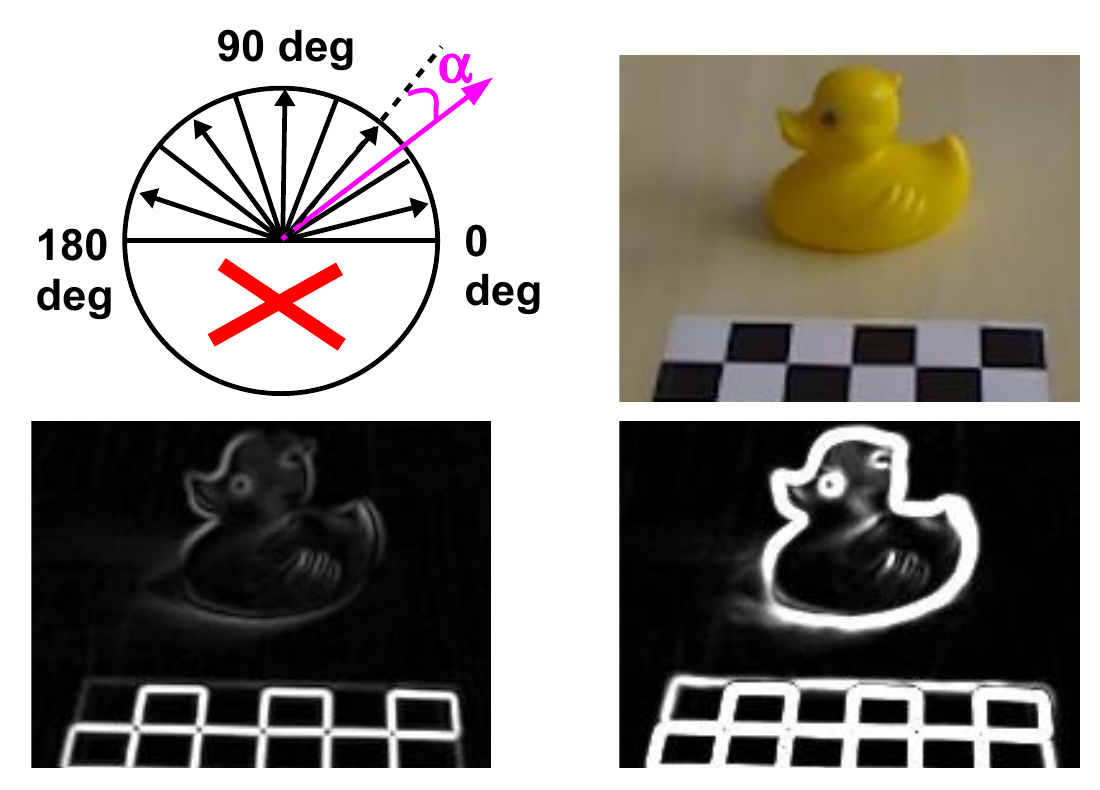
\includegraphics[height=2.5in]{./Graphics/duck-gradient}
\caption{Approximation of the gradient for the image of a duck toy:
  the quantization algorithm used by Line-MOD (right) provides a
  much better edge recognition performance with respect to standard
  algorithms (left). Image courtesy of Stefan Hinterstoi\ss er. \label{fig:duck-gradient}}.
\end{figure}

By considering only the direction of the gradient, and not its
full vector, two problems are solved: first, the gradient extracted
from the template will be compatible with the matching one,
independently of illumination changes. Second, by not taking into
account the way of the gradient, it will be valid both if the shape
stands on a dark background, and if it stands on a clear background:
the gradient will, in this case, maintain its module and direction and
only change its way, which will be discarded.

Regarding normals' quantization, the same considerations can be
applied. Dropping the normal vector's magnitude comes naturally, as
it will be $1$ by definition. Thus, again only the direction of the vector is
considered. Being a 3D vector, opposed to the 2D vector which is the
image's gradient, it is more difficult to find a good quantization function
for the possible values. The solution of \cite{linemod-paper} is to
quantize the normals' direction with respect to a set of possible
directions over the edges of a right, circular cone pointing towards
the camera. Each vector is then first flattened to the edge of the
cone, then to the nearest sample: in this way, the obtained value
is a representation of the radial direction in which the normal is deviating from the
camera's axis, which is a reasonable definition for what the normals
conceptually mean. Also, using a cone as a reference surface allows to
have a higher approximation level with a lower number of discrete
quantities, as each vector spawning the same radial direction
(longitude) will be well-represented no matter its latitude.

As depth sensors suffer from measurement noise, especially on the high
distances, after computing each pixel's normal vector and assigning a
quantized value to it, a convolutionary filter is applied to the whole
image: for each pixel, the local $5\times 5$ neighbourhood is
considered, and to that pixel is assigned, as a final depth value, the
sample that occurs most frequently into it (nulled normal vectors are
not considered at this step). This is useful as,
considering the surfaces as mostly smooth over a small area (sudden
changes in depth have been already removed by the normals' computation
step of sec.~\ref{sec:linemod-depth}), a voting algorithm can further
help with outliers' removal.

The result of this process can be seen in fig.~\ref{fig:depth-man}:
the man figured into the top-left corner has been captured with a
depth camera, and the resulting depth function can be seen in the
bottom-left corner; applying this quantization algorithm to the depth
map returns a result which is perfectly capable of distinguishing
different objects' borders (on which the image has been cut) and at
the same time subdivide smooth areas between each other.

\begin{figure}[htbp]
\centering
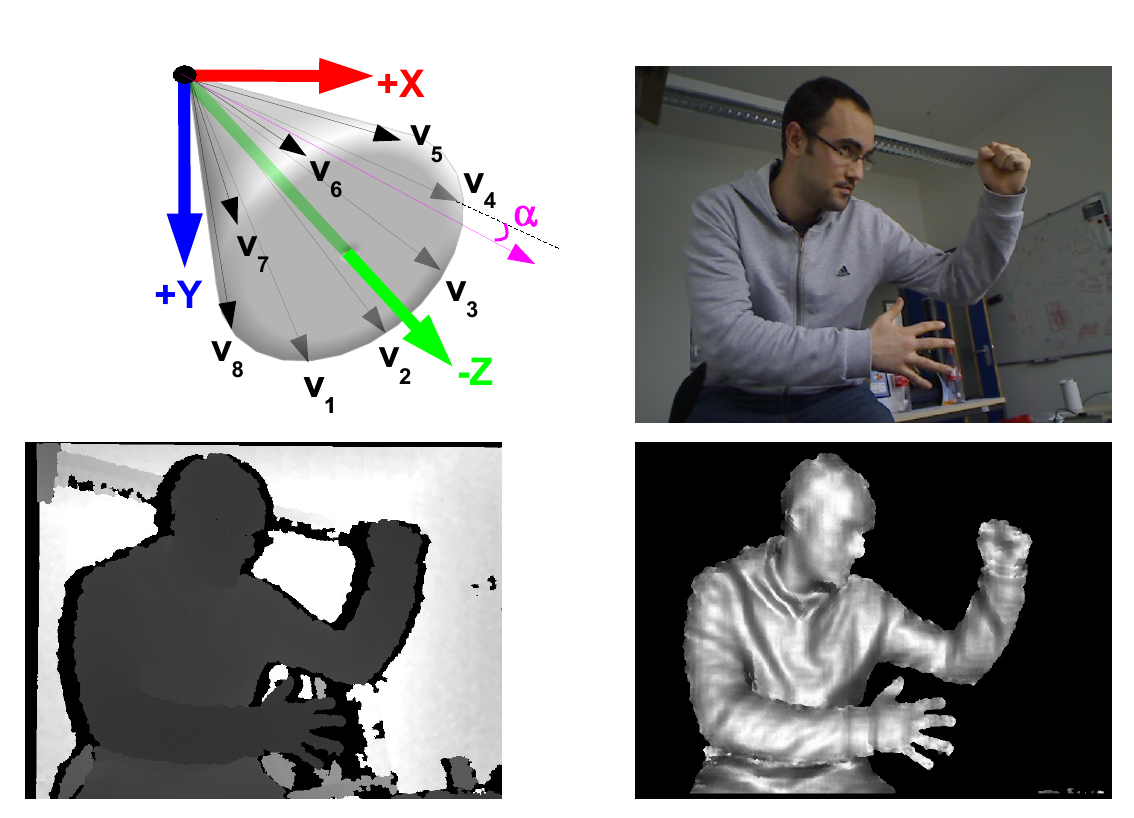
\includegraphics[height=2.5in]{./Graphics/depth-man}
\caption{Quantization of the possible values for a surface's normal
  vector to the surface of a circular cone (top-left). If applied to a
  real image (top-right), the input depth map (bottom-left) produces a
  normal map (bottom-right) which is already aware of difference
  between objects and can reproduce a good level of detail with
  respect to the original scene. Image courtesy of Stefan Hinterstoi\ss er. \label{fig:depth-man}}.
\end{figure}

\subsection{Binary representation of quantized images} \label{sec:linemod-binary}
After the images have been quantized, they are ready to be encoded
with a binary format, which is suitable for fast template
matching. Each quantized feature, being it gradient orientation,
normal orientation, or a custom one, is assigned to a $N$-bit value
($N$ representing the number of quantization levels), corresponding to
the value having a $1$ into one of its bits and $0$ into the other
ones: this allows a unique representation of both single values and
set of values. After this,
the values are ``spread'' in the neighbourhood of their corresponding
pixel. In simple term, each binary pixel from the previous step is
transformed into a binary pixel containing informations about which of
the quantization levels are present into the neighbourhood of size
$T$. At binary level, this is very easy and efficient to implement
given how the values are represented: in fact, it is sufficient to
generate $T^2$ images, each one shifted of a different number of
pixels in the range $\delta p = \left\{\left[-\frac{T}{2},
  \frac{T}{2}\right], \left[-\frac{T}{2},
  \frac{T}{2}\right]\right\}$; the result of a general \texttt{OR}
operation between all of these images will have the required
characteristics, as it will be formed of pixels having $1$ in the bits
corresponding to the features' values which are present at least once in
the adjacent pixels.

Spreading pixels in this way has the advantage of introducing at no
cost a good flexibility and robustness in terms of rigid deformation:
in fact, it maintains locality of features, but at the same time
permits to match features with a good margin of skew: the value of $T$
can be reduced if the algorithm is thought to be too permissive, but
it should never be deleted as this would cause all features to be
fixed to their pixel, which would cause obvious problems -- at least
due to the quantization error of the camera in terms of $(u,v)$
coordinates.

When the most important features have been spread in their surrounding
area, non-null pixels are left; this is the final result of the
template creation process, and the corresponding template can be
stored in memory for future usage. It is important to notice that a
template is actually a \emph{collection} of these sets of pixels
(i.e. features): for an image $I$, the corresponding template built
from modality set $M$ is thus a set of sets, $T(I) = \left\{ S_m(I), m \in M \right\}$.

\subsection{Line-MOD runtime algorithm} \label{sec:linemod-usage}
With all the premises of the previous sections, the Line-MOD algorithm
can be described. Line-MOD is a subset of Line
(\cite{linemod-origins}), which takes the same processing steps of
Line and applies it to match multiple features, computed from
different modalities, in parallel (hence the name, for
\emph{multiple-MODalities Line}). After computing and quantizing
set of modalities, seen by the algorithm through a simple abstraction
layer given by these three operations (the process at the upper level
is thus, indeed, completely modality-agnostic), this algorithm
converts them to binary form and spreads them, as explained in
sec.~\ref{sec:linemod-binary}. Each binary image is at this point filtered
through a certain logic, given by the feature itself: for example,
considering the case of untextured objects, colour gradients can be
found mostly onto the external edges of the objects: thus, only these
are extracted after gradient computation, as this will improve a lot
the algorithm's performance without impacting the recognition
process. As explained in sec.~\ref{sec:result-tests}, this has been
found to work for most cases with an actual good performance improvement.
On the other hand, considering normals on the edges would for sure
worsen the performance in terms of recognition accuracy, as normals
are not well-defined in proximity of the borders. Thus, normals are
filtered out and only those strictly inside the object are
considered. As shown in fig.~\ref{fig:duck-linemod}, this
complementary set of features, which cover the entire object if summed
up, is the main reason of the good performance of this algorithm with
respect to its predecessor as demonstrated in \cite{linemod-paper}.

\begin{figure}[htbp]
\centering
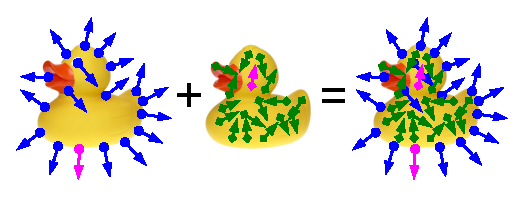
\includegraphics[width=4in]{./Graphics/duck-linemod}
\caption{Combination of different modalities, which is the main
  characteristic of the Line-MOD algorithm, allows to spread uniformly
  the detection of features upon the whole object, which is the main
  reason for its robustness. Image courtesy of Stefan Hinterstoi\ss er. \label{fig:duck-linemod}}.
\end{figure}

After feature spreading, each newly-created template is ready for
matching into an image. The scenario is thus changed from template
building to template matching, and the task to perform, for each
template $T$ which is put into a template list to be matched, is to
find a similarity measure $\epsilon_m (T,I)$ between the template itself
and a portion $P(I,c)$ of
the input image $I$, centred on $c$, on which the template has to be matched. Given a
similarity function $S_m(p_1, p_2)$ between two points $p_1$ and $p_2$
with respect to their quantized value with modality $m$ -- the ones
of which the templates' images are built -- the maximum similarity
score for each point in $P$ with respect to the corresponding
neighbour pixels in $T$ with maximum distance $r$ is taken, and these values are summed up:

\begin{equation} \label{eqn:similarity-function}
  \epsilon_m (T,I,c)=\sum_{p\in P(I,c)} { \left( \max \left\{ S_m
      (p,p_2) , p_2 \in P(c\dots c+r) \right\} \right) }
\end{equation}

Although similarity functions can be customized, the main ones used
by the Line-MOD algorithm consider the difference of direction between
corresponding pixels:

\begin{eqnarray}
  S(I,T,p_1,p_2) & = & \lvert \cos(\text{ori}(I,p_1) -
  \text{ori}(T,p_2)) \rvert \text{(for gradient)} \\
  S(I,T,p_1,p_2) & = & \lvert N(I,p_1)^{\tau} N(T,p_2)\rvert \text{(for normals)}
\end{eqnarray}

Here, $\text{ori}(I,p)$ indicates the orientation of the strongest
gradient of I at point p, as computed in
sec.~\ref{sec:linemod-gradient}, while $N(I,p)$ indicates the
approximation of the normalized vector normal to the surface of I as
computed in sec.~\ref{sec:linemod-depth}.

This is a good conceptual algorithm, but it would be enormously slow
if applied ad-litteram for each template and point into the image, as
it would require score computation for each point into the template,
each point into the image, each point into the neighbourhood; this
would lead to a cost of $O(\text{size}(I)\times \text{size(T)}\times
r^2)$, which is obviously unacceptable. A new data structure is used for
the purpose of matching, which is described below; usage of this
structure can lower drastically the computation time and bring it back
again to good levels.

The basic consideration for this is that the actual number $n_0$ of levels (bins)
on which each feature will be quantized, and thus the possible values
to which each pixel in the image will be matched, is actually really low; if,
for example, 8 bins are used to quantize values, after spreading the
binary representation of each pixel will be 8 bits, and thus contain
64 possible values. It is thus perfectly feasible to do a one-shot,
a priori computation of the score function $S$ for each possible
combination of input values. The spread image $I$ can be, in this way,
transformed into another serie of images $\tau_i(I), i \in 1 \dots 2^{n_0}$, resorting a lookup table, in
which each pixel corresponds to a list of values for $S$ which can be
easily matched with each possible value into the template $T$ by only
indexing it. Once this lookup tables has been built, the total
similarity function $S(I,T,c)$ will thus be much more easier to compute:

\begin{equation}
  \epsilon_m (T,I,c)=\sum_{p\in P(I,c)} { \tau_{I[p]} }
\end{equation}

It should be noticed that the lookup tables $\tau_i$ must be computed
only once, which reduces the computational effort of the matching
algorithm.

The result of this implementation is a fast (the computationally
intensive part has been reduced to direct memory accesses) and
versatile (the modalities can be of any type, as long as they provide
the characterising functions) matching algorithm, which can associate
to each couple $(T_i,p_j)$ of possible positions of a template into
the input image an output value which is a good representation of how
much the template fits well the chosen part of input. A natural but
important consequence of this is that no template will be flagged as
matching or not by the algorithm itself, so for example in case of light objects'
occlusions the ``good'' matches will find themselves to be the
ones with the highest score no matter the situation. After doing
this, it sufficient to discard every match for which the matching
score is below a chosen threshold -- which can be adapted with the
tradeoff of recognition capabilities versus potential false positives,
but will have no impact over performance -- in order to correctly
detect objects in every scene. With the same steps it is possible to
match more than one object type at the time, by simply putting more
than one template set into the list of templates to be recognized, and
assign to each a label indicating the object's type.

\subsection{Memory linearization for fast memory access on modern
  CPUs}
Being, for certain aspects, a quite low-level kind of algorithm, and
exploiting binary logic operations and intensive lookup tables access
for its matches, Line-MOD can improve a lot its performance by
exploiting the hardware features available to modern processors. In
particular, if the lookup table is not accessed properly, a high
number (near $100\unit{\%}$) of cache misses will impact heavily onto
the algorithm's performance. Line-MOD introduces thus the concept of
\emph{memory linearization} (from which the name \emph{Line} comes) to
ensure that, at matching time, the best possible sequence of pixels
will be matched in order to minimize cache misses.

One of the advantages of spreading the features' values as done in
sec.~\ref{sec:linemod-binary} is the fact that, if a feature is
present at point $p(u,v)$, it will be present also in all of its
neighbourhood of size $t$. As the similarity function only considers the maximum
value for each point into the considered pixel, it will be sufficient
to match one each $t$ pixels: if the point $p$ would affect this
maximum value, it will actually affect it being in a neighbourhood; if
it wouldn't, it can safely be ignored as it value would be obscured by
the maximum pixel's value.

Checking one every $t$ pixels would of course reduce the number of
steps by a factor $t^2$, but it would cause a lot of problems with
memory cache as stated above. Thus, the lookup table $S_i(I)$ is
reorganized in memory before matching by taking each $t$-th
pixel (i.e. creating a subsampled image starting at $p$) and storing it in a contiguous memory region, in a row-major
way; this will cause most of the image's salient points to fit the L1
cache of the CPU. When the subsampled image ends, the same process is
reiterated starting from the position following $p$. At the end of the
process, the whole image will be represented in memory in a manner
which is similar to how interlaced formats work, as shown in fig.~\ref{fig:linemod-linearize}.

\begin{figure}[htbp]
\centering
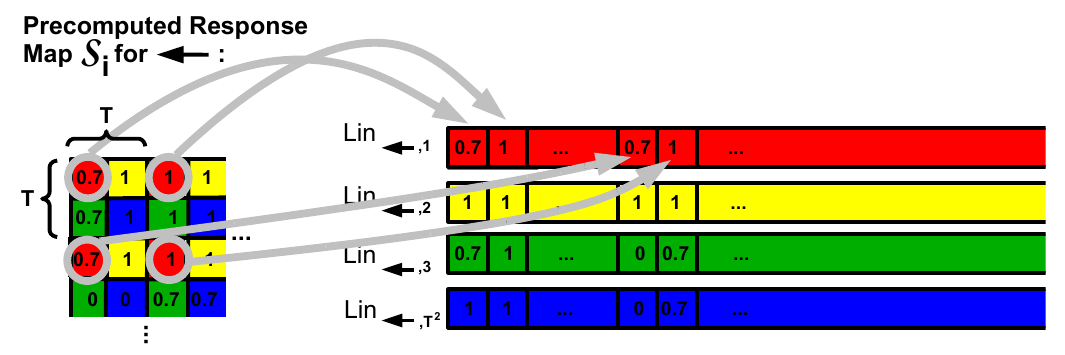
\includegraphics[width=5in]{./Graphics/linemod-linearize}
\caption{A precomputed lookup table $S_i(I)$ is, before matching,
  reorganized in memory so that the matching algorithm, taking one
  pixel every $t$, will seldom cause a cache miss. Image courtesy of Stefan Hinterstoi\ss er.\label{fig:linemod-linearize}}.
\end{figure}

\section{The iterative closest point (ICP) algorithm for 3D point clouds
alignment} \label{sec:icp}

A common problem when performing 3D point cloud analysis is the one of finding
matches between two sets of data, each sharing a partial set of points
corresponding to a part of the scene they refer to. After finding two sets of
matches which are known to correspond each other into the scenes, the
corresponding rigid transformation between the two can be computed. If one of the two
point clouds is then transformed using this transformation, the matches will
come in (almost) exact correspondence, and the two point clouds will then refer
to the same, global coordinate system. This problem is known as
\emph{point cloud registration} or \emph{point cloud alignment}. In this case,
the point cloud which must be aligned to a fixed scene is called \emph{data
cloud}, while the fixed point cloud, set into the global reference frame, 
which the data cloud must be aligned to is called \emph{model} or
\emph{reference cloud}.

If the scene is known to be still, this can be used to assemble together
different views of a same scene,
taken from different positions either by purpose or due to human error; in
fact, one of the most common use of registration algorithms is 3D scene
reconstruction starting from a set of views of the same scene. This is useful
for example in 3D scanning applications, where a 3D camera (like a Microsoft
Kinect) is moved slowly around an object and subsequent shots are taken;
after doing this, each image is registered to the previous one and a
bigger and bigger point cloud is obtained each time. When the last image is
reached, it is aligned to a known, ground-truth location to obtain a full
reconstruction of the scanned object in 3D global coordinates.

In this project, point cloud registration is used to find a transformation
between a computer-generated image -- the render of an object which is thought
to be recognized into the world -- and the real scene to which the image refers
to, i.e. the portion of image in which the object is thought to have been
found. The practical effect of this is that, if the object which will be
aligned to the scene is rendered with an associated, known pose, by applying
the resulting transformation the correct, refined pose of the object in the 3D
space can be found. This will be used in the later stages of the execution by
the gripper's algorithm.

Although numerous algorithms have been developed for 3D point clouds
registration, one of the most known and used ones remain the
\emph{Iterative Closest Point (\emph{ICP})}. Introduced first in 1992 in
\cite{icp}, the algorithm had sudden success into the computer vision
environment, due to its extreme simplicity, low computational cost and high
effectiveness. Numerous variants have been developed, which target either
computational efficiency, such the ones described in
\cite{icp-fast-algorithms}, or robustness with respect to certain parameters,
such as measurement noise, as in \cite{icp-bayes}, or a good compromise between the
two as in \cite{icp-robust}. The basic concept between these implementation
remains, anyway, always the same, and thus the processing steps stated in
\cite{icp} are taken here as a reference.

ICP is based on the assumption that, given a set of points with a good starting
guess for their reciprocal transformation, the point which corresponds to a
datum point into the data cloud is the one which is its
nearest neighbour in the reference cloud. At each instant within the
algorithm, a rough estimation of the transformation can be defined by computing
the transformation that would minimize the average distance between these
points. If the whole data cloud is then transformed using this transformation,
it will come closer to the reference; by iterating these steps several times a
solution can be found.

\subsection{Closest point computation}
First of all, the notion of \emph{distance} $d(\vec{p},C)$ between a point $\vec{p}$ in the data cloud
and a given model $C$ -- composed of $N_c$ model points $\vec{m_i}, i \in \{0 \dots
N_c\}$  -- is introduced:

\begin{equation}
  d(\vec{p},C) = \text{min}\left\{ E(\vec{p}, \vec{m}) : \vec{m} \in C \right\}
\end{equation}

Here, $E(\vec{x},\vec{y})=\lVert \vec{x} - \vec{y} \rVert$ represents the well-known
euclidean distance between two points. With this definition, the distance of a
point $\vec{p}$ to a cloud is given as the distance from $p$ to its closest
point within $C$. Using the same definition, the closest point $\vec{p_c}$ to
$\vec{p}$ is the point satisfying the equation $E(\vec{p},
\vec{p_c})=d(\vec{p}, C)$. Finding this point is an operation which can be done
with an average cost of $O\left(\text{log}\left(N_c\right)\right)$ using a K-D
tree as explained in sec.~\ref{kdtree}, and with a worst-case computational cost of
$O\left( N_c \right)$; thus, finding the complete set of closest points to
every point in the reference, i.e. finding the set $P_{c} = \left\{ p_c :
E(\vec{p},\vec{p_c}) = d(\vec{p},C) , p \in C \right\}$, has an average
computational time of $O\left( N_p \text{log}\left(N_c\right) \right)$, and a
worst-case one of $O\left( N_p N_c \right)$.

\subsection{Best transformation choice} \label{sec:icp-best-transformation}
After assigning to each point in the data cloud a correspondence within the
model cloud, the problem of finding the best transformation, which is the one
giving the least possible average squared distance between every point $p$ and
its corresponding point $p_c$, has two well-known solutions. 

In the case of 3D point clouds with no additional informations to register, a
good approach is the use of unit quaternions, i.e. quaternions $q$ which norm is
equal to 1:

\begin{equation} \label{eqn:quaternion}
q = \begin{pmatrix}a\\b\\c\\d\end{pmatrix}, a^2+b^2+c^2+d^2=1
\end{equation}

Unit quaternions are a well-known form of representation for rotations, which can
thus be combined with a translation to form a complete affine transformation
representing reciprocal pose\footnote{In this case, the scaling factor $s$ of
  the resulting affine transformation is assumed to be 1, as the registration is
  performed between clouds of the same scale (i.e. the registration process
results in a rigid transformation)}. Given the quaternion $q$ of
eqn.\ref{eqn:quaternion}, it can be univocally associated with a rotation
matrix, without redundancy:

\begin{equation} 
  R = \begin{pmatrix}
    a^2+b^2-c^2-d^3 & 2\left(b c - a d \right) & 2\left( b d + a c \right) \\
    2\left(b c + a d \right) & a^2+c^2-b^2-d^2 & 2\left( c d - a b \right) \\
    2\left( b d - a c \right) & 2\left(c d + a b\right) & a^2+d^2-b^2-c^2
  \end{pmatrix}
\end{equation}

If a translation vector $t=\begin{pmatrix}x_0 & y_0 & z_0\end{pmatrix}^{\tau}$
is combined with $R$, and this affine transformation is applied to the point
$p$, the resulting point $p_1$ will be:
\begin{equation}
  p_1=R*p+t
\end{equation}

Thus, in order to find the optimal transformation between the two clouds, $R$
and $t$ must be found so that

\begin{equation}
  S=\frac{1}{N_p}\sum_{i=1}^{N_p}\lVert p_{c,i} - Rp_i -t  \rVert
\end{equation}

is minimized.

It has been proven in \cite{extrinsics-algorithm}that the optimal rotation
quaternion $q$ can be found by first computing the centres of mass of the data
cloud $\vec{\mu_d}$ and of the reference cloud $\vec{\mu_r}$, then using these for
computing the cross-covariance matrix $\Sigma_{p}$ between the two points' set:

\begin{eqnarray}
  \vec{\mu_d} & = &  \frac{1}{N_p}\sum_{i=1}^{N_p}\left(\vec{p_i}\right) \\
  \vec{\mu_r} & = &  \frac{1}{N_p}\sum_{i=1}^{N_p}\left(\vec{p_{c,i}}\right) \\
  \Sigma_{p} & = &
  \frac{1}{N_p}\sum_{i=1}^{N_p}\left[\left(\vec{p_i}-\vec{\mu_d}\right)\left(\vec{p_{c,i}}-\vec{\mu_r}\right)\right]
\end{eqnarray}

After this, the matrix $A=\Sigma_{p}-\Sigma_{p}^{\tau}$ is built, and its cyclic
components are used to build a column vector $\Delta$. These data are used to
build the $4 \times 4$ matrix $Q$ shown in
eqn.\ref{eqn:q-of-extrinsics-algorithm}, and the best solution for $q$ is given
by the eigenvector of $Q$ corresponding to its maximum eigenvalue.

\begin{eqnarray}
  A & = & \Sigma_{p}-\Sigma{p}^{\tau} \\
\Delta & = & \begin{pmatrix}A_{2,3}\\A_{3,1}\\A_{1,2}\end{pmatrix} \\
  Q & = & \begin{pmatrix}
  \text{tr}(\Sigma_{p}) & \Delta T \\
  \Delta & \Sigma_{p}+\Sigma_{p}^{\tau}-\text{tr}(\Sigma_{p}I_{3}) 
\end{pmatrix} \label{eqn:q-of-extrinsics-algorithm}\\
q & = & \left\{ \vec{x} \in \text{Eigenvectors}(Q) :
  \text{Eigenvalue}(x)=\text{max}\left(\text{Eigenvalue}(x)\right) \right\}
\end{eqnarray}


After finding the rotation matrix $R$ as described above, it has been shown that the best solution for $t$
is for it to be the translation vector between the centre of mass of the
reference cloud $\vec{M_{r}}$ and the one of the rotated
data cloud $R\vec{M_d}$ 

\begin{equation}
  t = \vec{M_r}-R\vec{M_d} =  \frac{1}{N_p}\sum_{i=1}^{N_p}\left(\vec{p_{c,i}}-R\vec{p_{i}}\right) 
\end{equation}

With this procedure, best transformation between corresponding point clouds can
be found in $O(N_p)$ steps.

\subsection{Iterations and ending conditions}
The ICP algorithm applies the two previous steps of nearest neighbour search and
best transformation computation iteratively, hence its name; at every step, the
relative pose between the two clouds gets better. This is not only an heuristic
supposition, as a theorem has been proven
proven in \cite{icp}, stating that the whole algorithm will converge
\emph{monotonically} to a minimum of the distance function: thus, every
iteration will yield to a better result no matter the current state of the
algorithm.

Two main termination conditions are used by ICP: the first is the best-case one,
in which the total distance between the two point clouds $R$ and $D$ becomes smaller than a
given threshold:
\begin{equation}
  d(D,R) = \sum_{i=1}^{N_p}\left(p_i,R\right) < t_{\text{good}}
\end{equation}

The second is a condition that lets the algorithm end if it is stuck in a local
minimum of the distance function: in this case, as the error will always
decrease as stated before, its variation will decrease too and eventually become
smaller than a certain threshold $t_{\text{stop}}$ at time $t$:
\begin{equation}
  \Delta d_t(D,R) = d_t(D,R)-d_t(D,R) < t_{\text{stop}}
\end{equation}

The whole algorithm can be then summed up in this way:
\begin{enumerate}
\item{Start with given data cloud $D$, reference cloud $R$, transformation
  guess $P$, last transformation $T=P$;}
\item{Transform each point $p \in D$ using the current transformation $T$;}
\item{For each point, search for the nearest neighbour $p_c \in R$ and create
  the set of associations $A=\left\{(p,p_c) : p \in D \right\}$;}
\item{Find the best transformation from $D$ to $A$ as explained in sec.~\ref{sec:icp-best-transformation}, and save it into $T$;}
\item{Stack the current transformations together into $P$: $P=TP$;}
\item{If $d(D,R)<t_{\text{good}}$ or $\Delta d(D,R)<t_{\text{stop}}$, exit;}
\item{Go to step 2.}
\end{enumerate}
\subsection{$K$-d Trees} \label{kdtree}
In order for the problem of finding the closest point $\vec{p_c}$ to $p$ not to
have fixed computational cost $O(n)$, a \emph{$K$-d tree} (i.e.
$K$-dimension tree) is used; it is
a data structure which extends to more than one dimension the concept of binary
partition tree. If a point cloud is organized using a $K$-d tree, its points
result iteratively sorted with respect to their coordinates, which allows a
faster division of the search space.

As in a binary tree, data inserted in a $K$-d tree is organized in a
hierarchical way. Each item in the tree is a single vector with $K$ dimensions.
Starting from the top node, called \emph{root}, navigation into the tree is done
top-down: nodes have two trees below them (called \emph{subtrees}), containing one
or more elements, called \emph{children}; children in the first (or \emph{left})
subtree are always lesser then their father's node, with respect to a certain
evaluation function, while children in the second (\emph{right}) subtree are
greater\footnote{The case in which an exact duplicate of a datum is inserted is
 not covered here, as it is assumed that the point cloud to be transformed in a
 $K$-d tree is sparse enough.}. The discriminant function for a given node is usually chosen to be an hyperplane, to
which the node belongs to: in
this way, the whole points' space is, at each level, subdivided in half. Thus,
points which belong to the same subtree are spatially near each other.
Fig.~\ref{fig:kd-tree-subdiv} exemplifies this concept.

For 3D data, the choice of the hyperplane can be different at each level of
subdivision: the dividing plane is usually chosen to be parallel to the X axis
for the first level, Y axis for the third level, and so on; this makes the
discriminant function very lightweight, as it only consists of comparing one of
the coordinates of the object to be inserted (or searched for) with the same
coordinate of the current node.

\begin{figure}[htbp]
\centering
  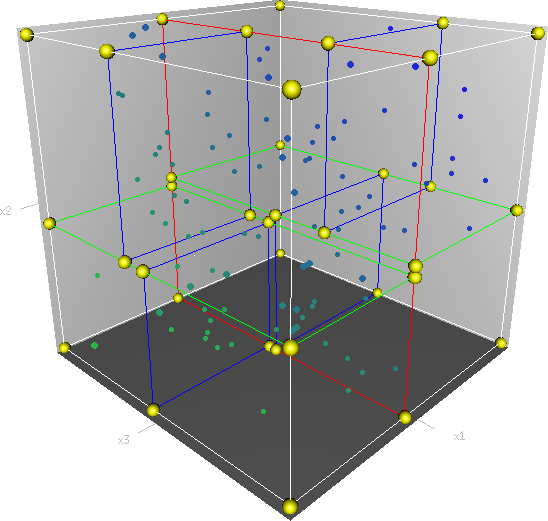
\includegraphics[width=2.5in]{./Graphics/kdtree} 
  \caption{A $K$-d tree recursively subdivides the data space in smaller
  hypercubes by means of hyperplanes: thus, points belonging to the same subtree
  are spatially near to each
  other. Image source:
https://upload.wikimedia.org/wikipedia/commons/b/b6/3dtree.png (GNU GPLv2)  \label{fig:kd-tree-subdiv}}
\end{figure}

If a new value must be inserted into a list, the usual rules of BSTs apply:
the value is compared with the root node, and the insertion algorithm moves to
the left or to the right subtree based on the result of this comparison. This
process is reiterated, and the
value is inserted when the algorithm reaches a node which has no subtree into
which to move further (\emph{leaf}). The problem with this approach is the
possibility of building a tree which is not \emph{balanced}, i.e. with a much
higher number of nodes in one of the subtrees with respect to the other. However,
when building a $K$-d tree out of a point list, the insertion algorithm can sort
the elements to be added before starting: in this way, a balanced tree is easier
to build, as it is sufficient to choose, for each subtree, the median element of
the data as the root.

When the whole tree has been built, it is easy to exploit its properties to
simplify the operation of nearest-neighbour search for a datum value. The
algorithm is recursive, and proceeds by searching the nearest neighbour in one
of the subtrees, then exploiting the properties of $K$-d trees to avoid
computation on the other subtree if not strictly necessary. In practice, given
the point $\vec{P}=\left(p_0,p_1,\dots,p_n\right)$, it goes
as follows:

\begin{enumerate}
  \item{At start, set the distance of the nearest neighbour to be $d=+\infty$
    and the root of the tree as the current node;}
  \item{the nearest neighbour is the root node if the tree has only 1 element
    (termination condition);}
  \item{if the current node $\vec{C}=\left(c_0,c_1,\dots,c_n\right)$ has a lower distance than the best one, set it as
    the nearest neighbour;}
  \item{search the nearest neighbour (recursion step) into the tree $T_1$ to which $\vec{P}$
      belongs to, i.e. into the left tree if $p_i < c_i$, into the right tree
    otherwise; update $d$ if a new nearest neighbour has been found;}
  \item{using the current best distance, examine whether the other branch $T_2$ of
      the tree has to be examined. This is the \emph{crucial} step of the
      algorithm, being the one that makes it better with respect to the trivial
    ones. Geometrically, the other branch of the tree must not be examined if no
    point lies on the other half of the space such that it is contained in the
    hypersphere centred in $\vec{P}$ and with radius $d$; however, for how the $K$-d
    tree is structured, it can be seen that this definition is equivalent to
    saying that the same sphere does not cross the division hyperplane generated
    by $\vec{C}$: this, in turn, is equivalent to saying that the distance from $\vec{P}$
    and $\vec{C}$ (taking only the $i$-th coordinate into account) is less than $d$:
    \begin{equation}
      \not \exists \vec{x} \in T_2 : \lVert \vec{x}-\vec{P} \rVert < d
      \Leftrightarrow \lvert c_i-p_i \rvert < d
    \end{equation}
    if this property, which is shown in fig.~\ref{fig:kdtree-hypersphere}, does not apply, search recursively into the other branch
  $T_2$ as well.}
\end{enumerate}

\begin{figure}[htbp]
\centering
  \adjustbox{valign=m}{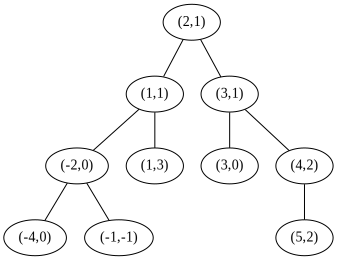
\includegraphics[width=2in]{./Graphics/kdtree_graph}} 
  \vspace{0.5in}
\begin{tabular}{c|c}
  \adjustbox{valign=m}{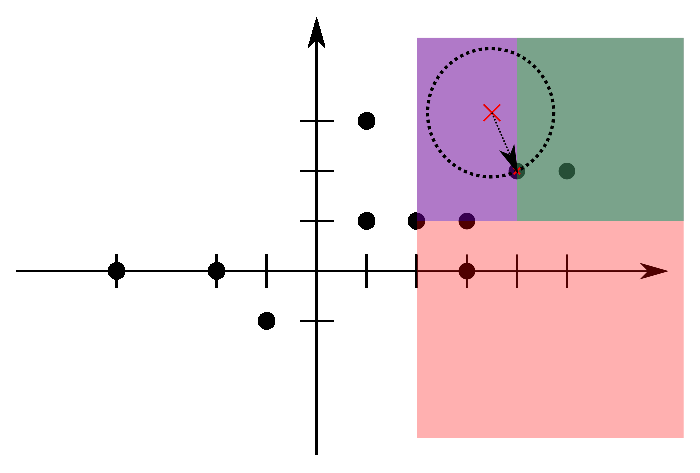
\includegraphics[width=2in]{./Graphics/kdtree_plane_2}} &
  \adjustbox{valign=m}{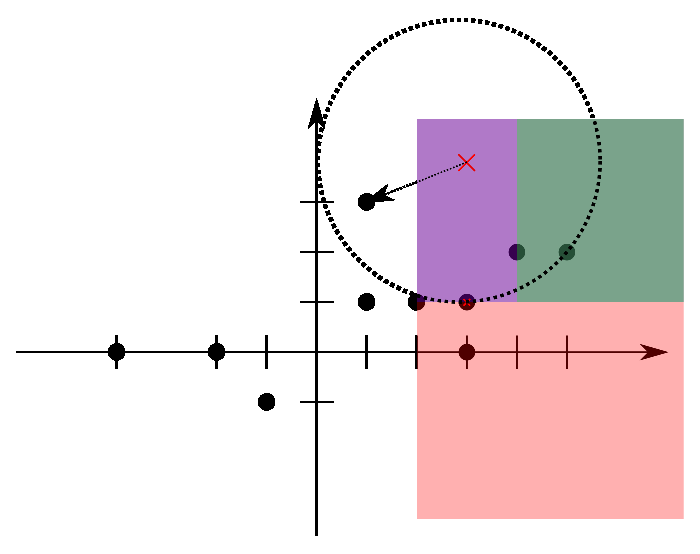
\includegraphics[width=2in]{./Graphics/kdtree_plane_1}}
\end{tabular}
    \caption{A $K$-d tree, like the one shown on the top, subdivides the
      points' space based on points' coordinates. If the distance from a point
      $\vec{P}$
      to an hyperplane is less than a value $d$, then no points on the other
      half of the space have a distance smaller than $d$ to $\vec{P}$ (left). If
      there is such a point, the distance from the point to the plane is smaller
    than $d$ too: this means that the hypersphere centred in $\vec{P}$ of
  radius $d$ crosses the plane (right). \label{fig:kdtree-hypersphere}} 
\end{figure}

Exact computational analysis of this algorithm is quite tricky; however, it is
intuitive to see that, given a well-balanced $K$-d tree and a point chosen
randomly, the algorithm will skip processing half of the tree about one half of
the times: this gives an average  execution time of $O(\log N_p)$, as stated
before.


\section{Recognition and pose estimation pipeline} \label{sec:linemod-pipeline}

In this chapter a pipeline similar to the one introduced in
\cite{linemod-pipeline} is presented, which is used to detect and estimate
the pose of the objects to be recognized. First a template matching approach is
used to detect the objects, then matches are progressively excluded (false
positives detection) based on hue values; finally valid matches are
progressively refined by physically moving a precision depth camera and
performing depth-based alignment of the match and the real object.

\subsection{Image matching using the Line-MOD algorithm} \label{sec:match-with-linemod}
The proposed object recognition algorithm is started by an upper
algorithm, managing the whole gripping strategy, which requires to the
recognition system to find a set of known objects into an RGBD
image. Three images are actually passed for recognition, which are
assumed to be registered at a pixel level: the RGB image of the scene,
the corresponding depth image, and a mask. The latter is an 8-bit
image with the same size of the whole scene, having each pixel with
value 255 if the pixel must be evaluated for recognition, and 1 if it
must be discarded.

For each object, the recognition system can be instructed to use a
recognition algorithm different from Line-MOD: if it isn't, the object
is assumed to correspond to a valid object for the Line-MOD
training database. This is the case which is treated in the rest of
this section.

For each model which has to be recognized using Line-MOD, the
corresponding training database is read from memory; this database
is created at initialization time from a directory tree which
associates each object's ID with the corresponding detector
description (number of modalities, type of modalities, mesh used for
rendering the object, etc.) and with the list of templates which are
associated to the object. After reading the objects, all of their
templates are merged together to form a single template list which
will be used for matching: information about the nature of each
template is maintained inside the template itself, as each item of the
list contains both the template's features and some metadata, like the
object ID the template refers to, the pose of the object which
corresponds to it, and additional informations which can were saved
during training (for example, if a simple filtering algorithm for false
positives  based on RGB histograms has to be implemented, it is enough
to link these data to the templates when training, and they will be
easily recovered when matching); the features of the image which is
included into the input mask are then computed, their binary
representation and response map are generated as described in
sec.~\ref{sec:linemod-binary}, and each template is matched upon
this. As the most intensive part for Line-MOD is the computation of
the response map for the scene's image, while template matching is
almost instantaneous, it is very convenient to match all the possible
templates in a single pass, as this will require the scene image to be
processed only once.

For each match, a corresponding matching percentage is defined. Given
the similarity function of eqn.~\ref{eqn:similarity-function}, the
percentage $S_\%$ of match for each template $T$ can be easily defining by noting
that the maximum possible similarity score, given when the two
images match perfectly, is given by the similarity function of the
scene's section $I$ with itself:

\begin{equation} \label{eqn:match-percentage}
  S_\%(T) = \frac{S(I,T)}{S_{max}(I)} = \frac{S(I,T)}{\sum_{p \in I}
    \left( \tau I_{p} \right)}
\end{equation}

In order to avoid considering matches which bring too little
information due to the extremely low matching area, a filter is put on
all the matches that come out from this cycle, checking both the
matching percentage defined in eqn.~\ref{eqn:match-percentage} to be over
a threshold $t_\%$ and the total area (in pixels) of the template
which matched to be over a threshold $t_{\text{area}}$. All the
matches that pass this check are kept as valid and stored into a
match list.

When this loop exits, thus, it will output a list of matches which are
tolerably strong and matched with a valid object pose and ID.

As it operates on multiple objects at the same time, this algorithm
will make sure to find at least a valid match for each object before
exiting; if this does not happen at the first iteration, the
Line-MOD algorithm is started again, and the minimum similarity
threshold $t_\%$ is decreased by a factor 0.95; matches (which can
uniquely identified by the object ID, template ID, and matching
coordinates $(u,v)$) which have already been processed will be
discarded in the following loops in order not to count them twice.

\subsection{Pyramidal matching for faster match}
As with most of the vision algorithms operating on medium-sized (VGA)
to large-sized  images, it is often inconvenient to process the
whole source image each time a detection query is made from a part of
the program. The solution used in this cases to significantly speed up
the performance of the recognition pipeline is the usage of
\emph{image pyramids}.

If pyramids are used to process a sample, the recognition algorithm
doesn't actually process the whole if it: instead, before recognition
a set of derivative images are built from the source one, each of a
smaller scale (usually, halved scale), until a predefined scaling
level is reached. In order not to lose too much information,
especially regarding image's features -- which, by definition, often
are present only in a narrow range of the image -- scaling
is not done roughly by downsampling the image: instead, first the
full-scale image is blurred using either a \emph{gaussian} or
\emph{laplacian} transform, and downsampling is done only after this
step. The images' set (the pyramid) is built top-down, iterating over
the lowest-scale image to produces the subsequent one; the mathematics
behind this transformations has been well studied in literature and is
omitted here, a good explanation for it can be found in most computer
vision books such as \cite{computervision}. An example of the pyramidal
images' building process is seen in fig.~\ref{fig:pyramidal-images}.

\begin{figure}[htbp]
\centering
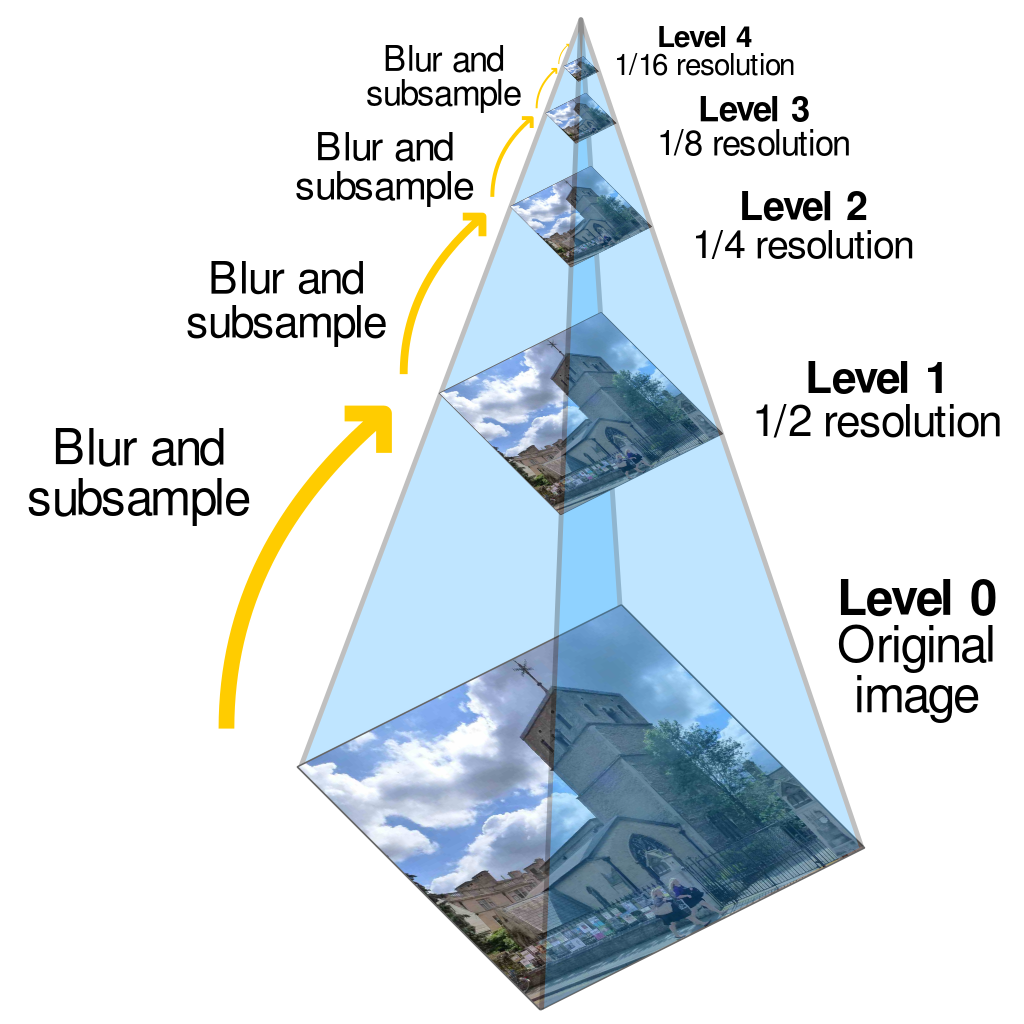
\includegraphics[width=3in]{./Graphics/pyramidal-images}
\caption{Building an image pyramid from an image: at each iteration,
  the top level of the pyramid (i.e. the image with the smallest
  scale) is blurred and downsampled to produce the next pyramidal
  level. Image source: Cmglee (own work) (CC-BY-SA 3.0)
  \label{fig:pyramidal-images}}
\end{figure}

The Line-MOD algorithm's implementation used into this project, based
on the one implemented into the OpenCV libraries, actively uses
pyramidal matching in order to speed up its operation. When an
object's model is requested to create and store a Line-MOD template
for subsequent usage, it takes the input images and creates a
two-levels pyramid from them. It then extracts features and template
data for both levels; in this sense, a template for this detector type
is actually a set of templates, each operating at a different
scale. When the detector is told to use its informations to
match templates over an image, filtering matches with a certain
confidentiality threshold $t$, it first builds the same pyramid from
the source image, and searches for template matches on it. Templates
are accepted only if they match within a certain threshold, which is
set to a fraction of $t$ in order to sustain the loss of information
that the lower scaling factor brings with it. Although the matching
threshold is lowered at this step, this already helps a lot in
discarding templates which are not present into the source image, and
thus fastens the operation, as matching at each subsequent pyramidal
level means having one order of magnitude less of complexity in
matching.\footnote{although matching templates is an almost
  instantaneous operation, the big number of templates which have to
  be matched into the image has to be considered}. Only the templates
which survive this first matching step are matched against the
full-scale image; also, as matching at a deeper level already gives a
good hint about where each template could be present into the whole
image, when matching at full scale only those parts which are within a
small radius with respect to the previous match's origin have to  be
searched, which brings to further performance improvement on the algorithm.

The important thing to notice about all of this process is that,
starting from full-scale images (when recognizing) and templates (when
training) the whole process is \emph{totally transparent} to the user:
this is an obvious advantage as the user probably will not be willing
to further manipulate its source images when matching if not strictly needed.

\subsection{False positive rejection based on hue values}
The first step of pose matching is made by purpose to be overly tolerant in
template matching. This is because the used objects are quite small and simple
in shape - which can reduce the number of features to match - and at the first
step are seen from far away (more than 1 metre) in order to maximize the
field of view without increasing the needed number of cameras. The counterpart
for being sure to match \emph{at least} something is having a huge number of
  false positives, which must be recognized and excluded before starting the
  alignment.


To do this, after performing each match together with a rough pose estimation,
the object is rendered again into its estimated position, and the portion of
source image corresponding to the render is taken. The two images are then
compared on a per-pixel basis, considering only the pixels that lie on the
depth mask created during rendering. 

Before comparing, the two images are converted to the HSV colour space, and
comparation is done based on the hue values. This allows to only consider the
actual colour of the model and match, and discard all information about
surface behaviour with respect to light, together with variations in the images
depending on different lightning conditions.

HSV colour space has singularities on the hue dimension when the chosen pixel is
either black or white; in this case, in effect, the hue of the pixel is
undefined due to the low saturation or low luminosity (\emph{value}). To fix
this, white and black pixels are turned to be zero-saturated, zero-valued
pixels with fixed hue, corresponding to yellow (for white) and blue (for
black). When matching, these are treated as special values and two pixels are
said to match either if their actual hue match (which
is robust to moderate lightning changes) or if their modified hue, saturation
and values match
(which happens if both the model and the scene appear to be actually white or
black). 

After computing the new HSV values, the four resulting images (two belonging to
the source image, two belonging to the rendered one) are scaled down of a
factor $K_s$. This makes the four images to be downsampled, and improves the
success rate of the subsequent step as it does minimize small alignment errors
due to the pose estimation error within the template. The render's mask $m$ is
scaled down of the same factor.

After scaling, the mask is first filtered in order to keep only the points for
which the mask's value is 1 (thus correcting the interpolated values on the
border which come out of the scaling algorithm) and then
eroded by a small amount (1 pixel). This allows to further remove the noise
which usually comes into the object's borders.

Finally, for each pixel belonging to the newly created mask, a comparison if
done between the corresponding render's and scene's pixel. If their difference
is below a certain threshold $t$, the two pixels correspond. The corresponding
pixels are counted and the matching ratio $P_{match}$ is computed with respect to the
total number of pixels belonging to the scaled mask:

\begin{equation}
P_{match}=\frac{\text{count}\left[(u,v) : m_{u,v}=1 \wedge \left( \lvert
\text{Hue}(r_{u,v})-\text{Hue}(s_{u,v})\rvert < t \vee R_{u,v}=S_{u,v} \right)
\right]
}{\text{count}\left[ (u,v) : m_{u,v}=1 \right] }
\end{equation}

Here, $r$ indicates the scaled-down render, $s$ indicates the scaled-down scene
portion, while $R$ and $S$ indicate the corresponding images with modified hues.

The whole matching and filtering part is repeated until at least one match
passes the filtering step. If no valid matches are found during the first
iteration, the threshold level for the LineMOD algorithm is decreased
just like it was done in the previous step of the pipeline; in this
way, objects with small, partial occlusions can be recognized.

If the threshold $t_\%$ falls below a threshold $t_{\%,\text{bad}}$
and no valid matches have still been found to pass this check for every object, however, the
algorithm exits anyway: experimental tests have, in fact, shown that
when the matching threshold becomes below about $80\%$ the algorithm
tends to recognize almost every template as matching, but it will
still fail to recognize correctly the object in its correct
position. This will lead to a huge number of false positives (about
$50\%$) of the total templates, and the hue matching step described in
this section will in turn last several minutes just to continue
failing, which is a situation to avoid. 

\subsection{Point cloud alignments and pose refinement}
The matches that passed the first false-positive rejection step are saved and
sorted based onto their matching percentage. At this point, matches are probably
valid, but only colour information has been considered. Also, a good pose
approximation has been obtained for each match, but coming from a template, it
is not precise enough to be used for grasping. To overcome these problems,
another step is required for each match, which is pose refinement through point
clouds' alignment. In this step, colour information is dropped, and only depth
information is used. 

The Microsoft Kinect RGBD camera provides good depth informations for the template-matching
requirements, but it is not suitable for precisely find the pose of an object
for grasping. This is due mainly to the limitations of its depth sensor, having
a nonlinear depth error of about $1\%$.
Although this is quite a standard error, it must be combined with the minimum
depth range of $80\unit{cm}$ for the sensor. This leads to an error of about
$1\unit{cm}$ on the depth's values at medium ranges, as shown in \cite{kinect-evaluation}. Also, the field of view of the (fixed)
kinect does not allow to precisely detect the object's pose, as the depth error
increases the more the object is not centred with respect to the sensor. As a
higher precision is needed for good 
object grasping, a dedicated, precision depth sensor (\emph{Structure Sensor by
Occipital})has been mounted onto the robot's arm.


This camera's specifications\footnote{http://structure.io/developers} are much better than the kinect's ones, although it
does not provide RGBD images but only depth informations -- hence the need for two
different cameras; it has a much lower minimum range of $40\unit{cm}$ and is suitable for
precision depth measurements, having a maximum error of about $1\%$, which comes
down to $0.15\%$ at $40\unit{cm}$ of distance. This means having an absolute
error of less than $0.2\unit{mm}$ when the camera is close enough to the object.

As the matches already provided a good estimation of the object's position, the
iterative closest point algorithm explained into sec. \ref{sec:icp} can be
applied. 

First, the point cloud for the scene is obtained as explained in sec. \ref{sec:cloud-reconstruction}.
As explained, a scene's snapshot obtained by the precision depth
sensor used and the alignment process is done upon it. In order to
do this, the found match is rendered again into the position in which
it would be as seen from the camera -- whose extrinsic characteristics
are known because of the fixed locations of the bin; if this was not
the case, it would be enough to find it again at before rendering
using the algorithms of sec.~\ref{sec:camera-calibration}, as they
have negligible cost with respect to the whole recognition pipeline.
As the mask of the render has already been computed, it is exploited at this
point and only the part of the scene corresponding to the actual
object, increased by a low margin, is
transformed to a 3D point cloud.

During the process of 3D reconstruction a lot of invalid values can be
generated: these are the points for which the depth sensor failed to obtain a
valid measurement, and are ignored from this same algorithm. Two kinds
of values are dropped: those for which the depth measurement is
outside the range specified into the camera's specifications, which
is increased by a small margin to keep uncertainties into account, and
those for which the camera actually reports a $NaN$ value (e.g. in
case of a reflecting surface, for which the speckles patterns results
too heavily distorted).

Both the model's and the scene's cloud are moved to be in global
coordinates after reconstruction; this is done by transforming them
with the inverse of each extrinsic transformation.

When this is done, it will be very probable that the two clouds will
have different point densities, especially for the process of
information dropping coming from the recognition pipeline. This could
harm the premises of the ICP algorithm, as different point densities
or missing points could cause wrong correspondences between points.

To prevent this situation, after reconstruction and transformation,
both the point clouds are evaluated and filtered through what is
called a \emph{Voxel grid}. This filter creates a 3D grid of fixed
size through all the 3D space occupied by the point cloud, and
maintains the crossings onto the grid which correspond to the cells
occupied by at least one input point. In practice, this means that the
output of a voxel grid having a scattered point cloud as an input is
an approximation of the same point cloud made with \emph{equally
  spaced}, regular points. Using the latter instead of the first for
the ICP algorithm results in benefits to the proper
operation of the algorithm itself, as points' correspondence will
lead to zones of the clouds that actually correspond perfectly into the 3D space.

After tessellating the two point clouds, whose points are set in global
coordinates, the resulting filter outputs are aligned using Iterative Closer Point: if the
algorithm converges correctly, the cumulative transformation
$T_{\text{final}}$ of the ICP is used to transform the initial guess for the object's
  pose and obtain the final, refined pose estimation for the object.

Summing up all the points presented into this chapter, the proposed
system for object detection composes thus a complete system by its
own: in particular, the recognition pipeline is fully automatized and
can, starting from the two images taken from the cameras, arrive to
the estimation of the pose of different objects with sub-millimetric
precision. This system can thus be used with success into the solution
of the stated grasping problem.

\chapter{Object grasping via multi-object grasping strategy}
\section{Objects' representation and processing for best grasp computation}
After recognizing the objects which are present into the scene and having a
good pose estimation, the robot used for objects' picking must compute the best path
in which to travel in order to correctly grasp it. In this project, this task
is accomplished by simulating a set of predefined poses over each object before
gripping. As the goal of the project is grasping a \emph{set} of objects, a
good grasping strategy must be implemented too; this strategy is described in
detail in sec. \ref{sec:TODO}. However, this means that, independently from the
chosen global strategy, grasping pose computation has to assign to each
possible set of movements (which we will refer to as a \emph{grasp} from now on)
a \emph{score} representing the difficulty of picking
for that particular grasp. The chosen algorithm assigns to each grasp a
probabilistic score, based on the intersection volume between an emulated
gripper and the scene, from which the object to grasp has been removed.

In this section, first it is described the score concept (sec.
\ref{sec:grasp_score}), then the chosen way of modelling the gripper (and robot) and
the scene (sec. \ref{sec:shapes}). Finally, a flexible way to compute the score for a set of possible
grasps is presented, together with details for particular cases (sec.
\ref{sec:grasp_computing}).

\subsection{Probabilistic grasping score} \label{sec:grasp_score}
For the implementation of any high-level grasping strategy for multiple
objects, i.e. for the program to be able to correctly choose which object to
pick first at each time instant, a score has been assigned to each possible
grasp and for each possible object. For each pickable object, only the best
grasping poses are kept.

In order to well define the score (i.e. difficulty) of a grasp, which we will
indicate as $d$, a few
considerations have been done:
\begin{itemize}
  \item{First, an easy to do grasp with no obstacles
      into its path shall have score $d=0$. It shall, in fact, be  the preferred
    object for the high-level strategy to pick first;}
  \item{on the other hand, a grasp which puts the
      gripper at risk of hitting the borders of the object's container -- being them
      the edges of a bin or the floor -- shall have score $d=+\infty$. Trying to pick the
      object with this grasp could cause physical damage to the robot, the floor or
    even humans, thus the high-level strategy should discard it completely;}
  \item{if a grasp puts the gripper in contact with other objects of a scene, its
      difficulty can be evaluated by virtually assuming these objects will stay still and
      computing the intersection volume $V_{\text{int}}$ between them and the
      gripper for each of them;}
    \item{If the intersection volume $V_{\text{int}}$ is small enough to be
        under a certain threashold $V_{\text{easy}}$, the score could be assigned low enough for the
      grasp to be considered valid. In this way, if the gripper brushes the object
      without entering it completely, the grasp can be done, which in real situations
      will result in the gripper slightly moving apart the touched object without
    damaging it; }
  \item{the intersection volume, especially is considered to grow linearly, is not
      enough for evaluating the score: first, the score must grow consistently if the
      object is not touched only by the border but by a consistent part of the
      gripper, and finally saturate to $d=+\infty$ if the intersection volume
      reaches an acceptability threshold $V_{\text{max}}$. Also, as touching an object will result in moving it, grasp score
      should keep into account the actual difficulty of moving the intersected
      object. For example, bouncing with a closed, rigid box would probably not damage it
      also if the gripper enters it by a visible amount, while bouncing with an
      open book would almost for sure damage its pages. Thus, a \emph{movement
    coefficient} shall be assigned to each of the objects into the scene.}
\end{itemize}


With these considerations in mind, a suitable, global score function $s(V_{\text{int}})$
can be found. The score function must obey certain properties which can be
extracted from the above:

\begin{itemize}
  \item{The function must be monotonic and always positive;}
  \item{it must be linear when x is low enough, in order to evaluate
    lightly touches adequately;}
  \item{it must be continue in the whole domain: this does not come
      from the previous properties, but is needed in order to compute it without
    the need of caring about floating point's approximations;}
  \item{it must have a parameter $\alpha>0$ defining how much
    intersection volume globally affects hardness of grasp;}
  \item{it must have another parameter $K\geq1$ defining how much the hardness is
    increased rapidly after reaching the brushing threshold $V_{easy}$;}
  \item{when the intersection volume is greater than the brushing threshold, the
      function
    must never grow less quickly than when the volume is in the brushing
    region, i.e. $\text{max}\left( \left\{ \frac{ds(x)}{dx} | 0 \leq
    x \leq V_{\text{easy}} \right\} \right) \leq \text{min}\left( \left\{
  \frac{ds(x)}{dx} | x > V_{\text{easy}}\right\} \right)$.}
\end{itemize}

The chosen function, which satisfies all of the above properties, is

\begin{equation}
  s(V_{int})=\left\{
    \begin{array}{lcr}
      \alpha V_{\text{int}} & \text{when} & 0 \leq V_{\text{int}} \leq V_{\text{easy}}, \\
      \alpha
      \left[1-K\left(\frac{V_{\text{max}}-V_{\text{easy}}}{V_{\text{int}}-V_{\text{max}}}\right)\right]
      & \text{when} &  V_{\text{easy}} < V_{\text{int}} < V_{\text{max}}, \\
      +\infty & \text{when} & V_{\text{int}} \geq V_{\text{max}}.
    \end{array}
  \right.
\end{equation}

It is shown in appendix \ref{sec:TODO} that $s(V_{int})$ satisfies all
of the above properties for any $K\geq1$, and is thus suitable as a score
function. Some examples of this function varying the two parameters $\alpha$ and
$K$ are shown in fig. \ref{fig:score_function}.

\begin{figure}[htbp]
  \centering
  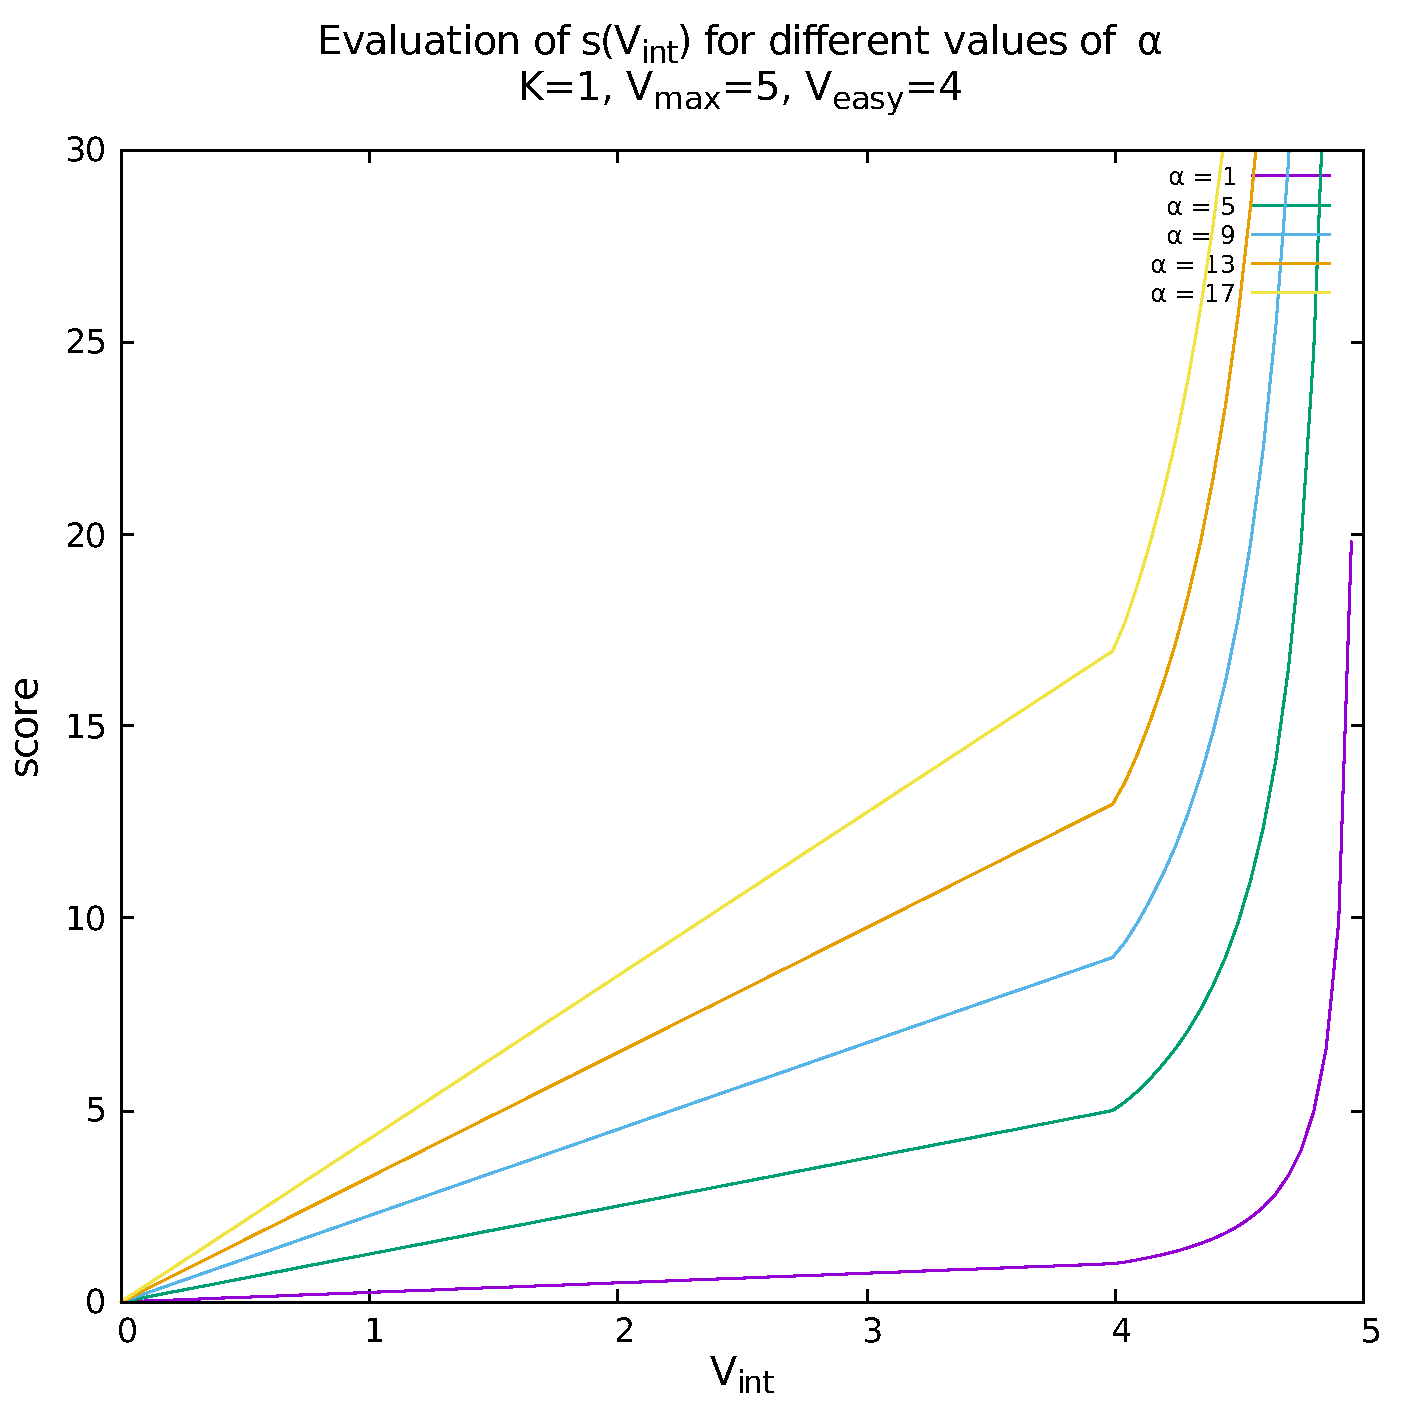
\includegraphics[height=3in]{./Graphics/score_alpha}
  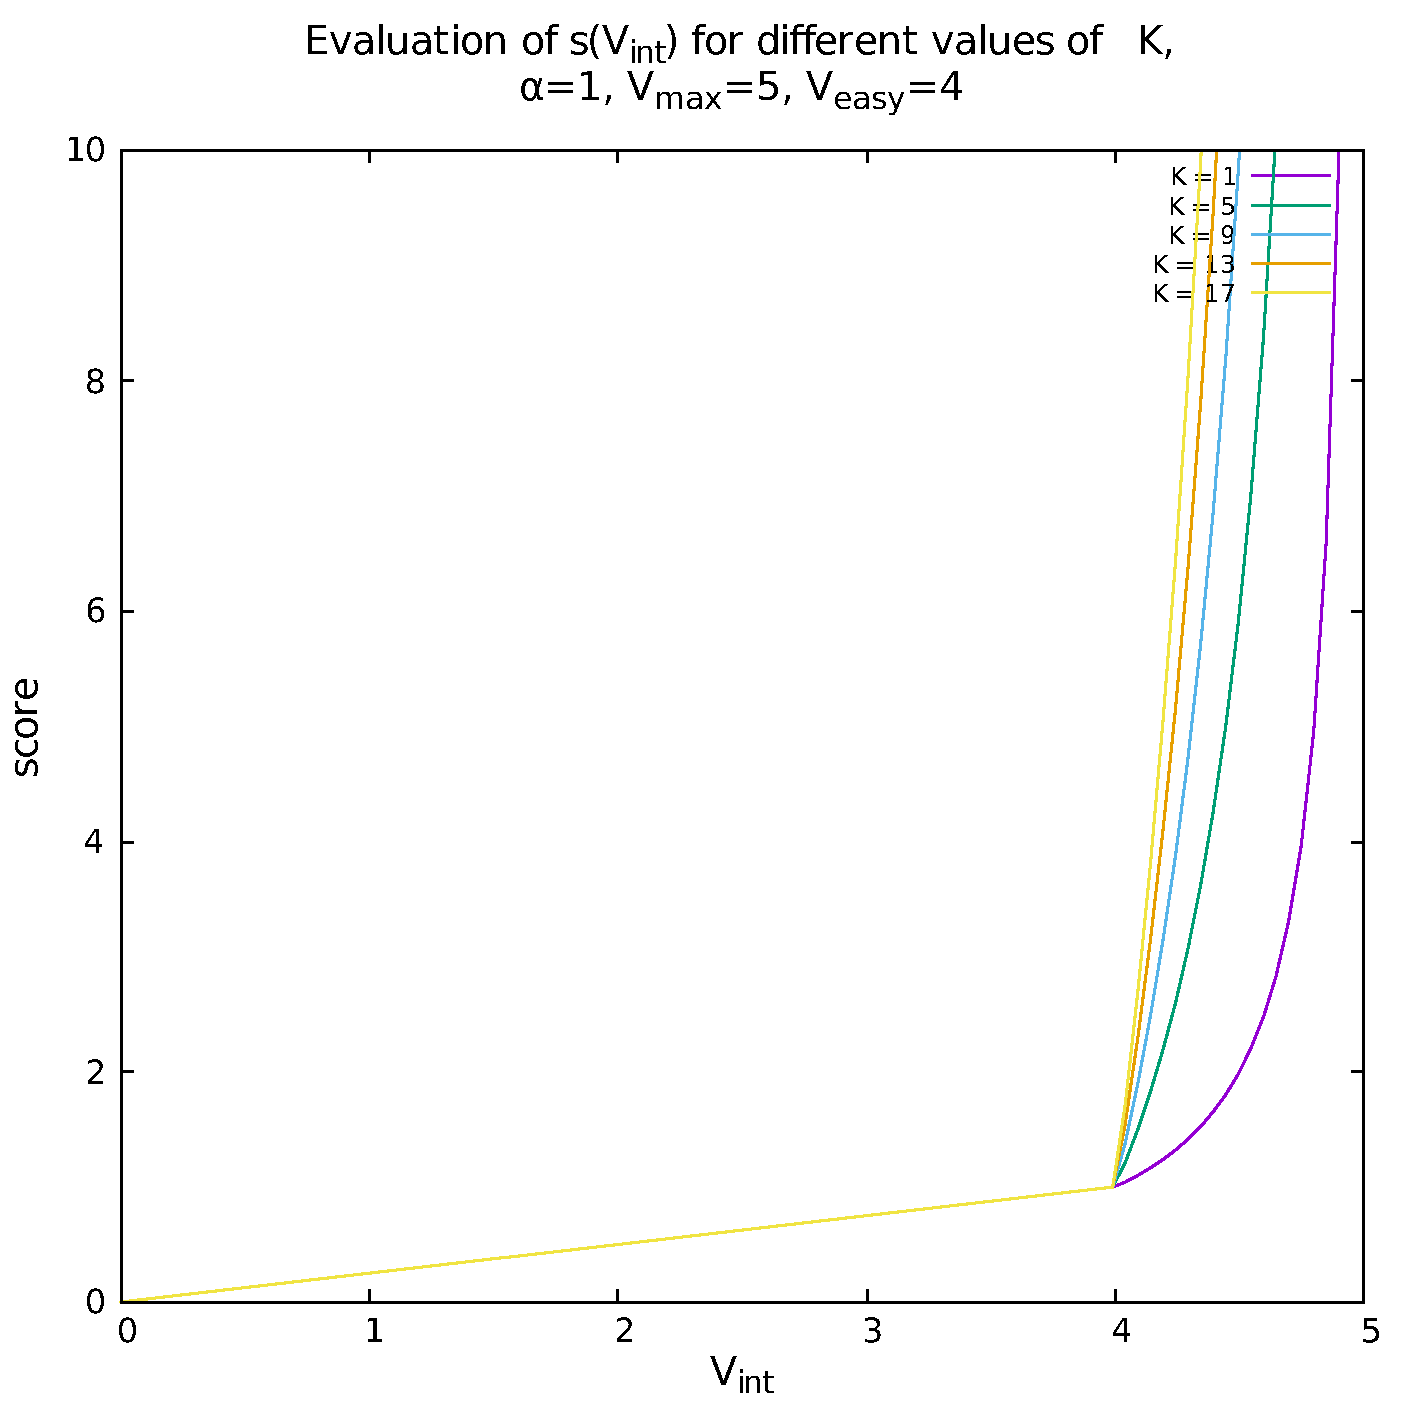
\includegraphics[height=3in]{./Graphics/score_k}
  \caption{Resulting score function for different values of $\alpha$ (top) and
  $K$ (bottom) \label{fig:score_function}}
\end{figure}

\subsection{Object representation as elementary shapes} \label{sec:shapes}
A good representation of objects is essential in order to compute efficiently
their intersection. In this project, objects have been represented by means of a
uniform data structure breaking down complex meshes to the union of simpler
shape, as done with the \emph{Constructive Solid Geometry (\emph{CSG})} tools of
most mainstream CAD applications. Each object is represented, for the purpose of
grasp computation, by means of simpler, basic shapes, associated to their pose
relative to the object's reference system. These will be called
\emph{primitives}. A tree structure can also be created
by considering compound objects created in this manner to be a shape type on
their own, thus allowing recursive object building. This is similar to what the
\emph{assembly} and \emph{group} tools of common CAD applications do, as well
as what the library used for mesh representation (Assimp) does for
multiple-nodes meshes. This approach has a serie of advantages:
\begin{itemize}
  \item{Every object shares a common data structure. This makes it easier for
      the intersection algorithm to be as general as possible with little to no
    effort;}
  \item{the tree representation of the object makes it easy to save single or
      multiple objects to file and to create objects' configuration by-hand,
      which is useful both for debugging and for execution purposes (for
      example, the database of objects, together with their shapes, can be made
    distributed with no effort and version control tools can be useful);}
  \item{using an approach similar to what is supported by CAD
      applications results in the possibility of scripting the latter in order
      to automatically produce an exact representation of the object starting
      from a CAD model, which could be the same used for training in sec.
    \ref{sec:cad-mesh};}
  \item{the approach is very flexible because of the relative independency
      between the object's model and the rest of the algorithms: new use-case of
      the algorithm (e.g. for moving or nonrigid objects) could leave this part intact, and
      only work by modifying the informations about the position of the whole,
    or part of, the object.}
  \item{new, complex shapes which have to be implemented in future can be added
      to the primitive shapes as an extension, without the need of rebuilding
      the whole objects' database. This is the main advantage of using an
      object-oriented approach based on polimorphism for the implementation of this
    part.}
\end{itemize}

For this project, four main shape types have been implemented, and with these
the whole set of objects kept in consideration have been succesfully
represented.

Each primitive is represented by its shape type and a set of dimensions, which
is checked at runtime to be coherent to the associated shape. To the shape is
associated a pose information, represented as an affine transformation as in the
rest of the project. To each shape type functions have been implemented to
recognize whether a it intersects with, or contains, a point, an edge, a line, or
another shape. When computing intersections, these are efficiently used as
special cases to recognize whether an intersection exists or not before
eventually running the computationally expensive intersection's volume
algorithm.

\paragraph{A \emph{cuboid}} is a shape representing a parallelepiped. It is represented by
three dimensions: its width $W$, its height $H$, and its depth $D$; its origin is fixed in one
of its corners, and its reference system's axis are on its edges' directions:
width extends over the $X$ axis, height extends over the $Y$ axis, and depth
extends over the $Z$ axis.

A point $P$ (in normalized homogeneous coordinates, i.e. with $w=1$  can be checked for belonging a cuboid $C$ of dimensions $(W,H,D)$ and
pose $A$ by first representing it into
the cuboid's coordinate system, and then checking its coordinates to be into the
cubes'dimensions:

\begin{equation}
P \in C \Leftrightarrow \begin{pmatrix}0\\0\\0\\1\end{pmatrix} \leq A^{-1}P \leq
\begin{pmatrix}W\\H\\D\\1\end{pmatrix}
\end{equation}
  
A line segment $L$ intersects the same cuboid if, by projecting it on one axis at a time,
all the three projections belong to the projection of the cube:

\begin{equation}
  L \in C \Leftrightarrow \left(L_x \in C_x\right) \wedge
  \left(L_y \in C_y\right) \wedge \left(L_z
    \in C_z\right)
\end{equation}

\paragraph{A \emph{sphere}} is a shape representing a sphere of fixed radius,
which is the only one of its dimensions. The reference system of the sphere, 
which its transformation refers to, is fixed into the sphere's center. Having
central simmetry, the rotation part of the sphere's transformation will actually
be ignored.

A point $P$ belongs to a sphere $S$ of radius $R$ if, after moving it into the
sphere's reference system, its distance from the origin is less then the radius:

\begin{equation}
  P \in S \Leftrightarrow \left(A^{-1}P\right)_{x,y,z}^2 < R^2
\end{equation}

Also, a line $L$ belongs to the same sphere if its distance from the origin is less
than $R$.

\paragraph{A \emph{cylinder}} is a shape representing a rect, circular cylinder.
Its two dimensional values represent the base's radius and the height of the
cylinder. Its coordinate system is fixed at the center of the circle, at the
base of the cylinder, with the
Z axis pointing upwards on the length direction.

A point $P$ belongs to a cylinder $C$ of radius $R$ and height $H$ if, after
moving it to the cylinder's reference system, its projection on the XY plane
belongs the base circle and its Z coordinate is lower than the cylinder's
height:

\begin{equation}
  P \in C \Leftrightarrow \left(A^{-1}P\right)_{x,y}^2 < R \wedge
  \left(A^{-1}P\right)_z > 0 \wedge \left(A^{-1}P\right)_z<H
\end{equation}

A line segment $L$ in the cylinder's reference system belongs to the same cylinder if its projection on the $XY$
plane belongs to the base circle and its projection over the $Z$ axis belongs to
the cilinder's height segment:

\begin{equation}
  L \in C \Leftrightarrow
  \left(L_{x,y} \in C_{x,y} \right)
  \wedge
  \left(L_{z} \in [0,H] \right)
\end{equation}

\paragraph{A \emph{compound}} is the composition of any number of shapes, called
\emph{children}. Children can be compounds too. This shape has no dimension
information, but only a reference system to which all the children's reference
systems are applied before any evaluation. For example, in order to transform a
point to a children's reference system for intersections' evaluation, the point
is first transformed using the compound's reference system, then it is
transformed again using the child's reference system. In this way, assembly-like
shapes can be formed.

A point, or any other primitive, $P$ belongs to a compound $C$ with children $c_i$ if it belongs to
\emph{at least} one of them:

\begin{equation}
  P \in C \Leftrightarrow \exists i : P \in c_i
\end{equation}

Using this four composing blocks, it is easy to form every object. Also, every
object can be evaluated for intersection with at least a point, which is the
base for the volumes' evaluation system described into sec.
\ref{sec:grasp_computing}; some objects can also be intersected more efficiently by
exploiting other special case features as line evaluation. Also, it has been
shown how the easy structure of each primitive, together with the use of
compounds, makes it easy to add further extensions to this system and immediately
make use of them.

\section{Efficient volume computation of objects' intersections} \label{sec:grasp_computing}
After defining the score function $d(V_{\text{int}})$, the only remaining
obstacle for computing the best possible grasping strategy is the actual
computation of shapes' intersections. In order to complete this task the problem
has been splitted on many levels: a trivial, resource-consuming -- but always
working -- algorithm to use whenever the actual volume must be computed and
there is no known better way to do it, a serie of heuristic algorithms to use if
the same problem can be brought to a closed-form, more efficient solution for
the shapes kept in consideration (e.g. for sphere-sphere intersection), and
another serie of heuristic considerations which can avoid the actual volume
computation if the problem is meaningless (e.g. when the chosen objects are
known to not intersect at all). 

\subsection{Point approximation of shapes on different levels of precision}
The basic algorithm is based on splitting one of the two shapes to intersect into a serie of cubes of
fixed dimension.
Cubes are then represented with their center only, and only this information is
used to compute the shapes' intersections' volume: for each cube, if the center
of the cube belongs to the other shape, the whole cube is considered to belong
to the latter. The final intersection volume is brought by the sum of the
volumes, actually approximating via Riemann's series the real value of the
intersection, as if it was
analitically computed by an integral. More in detail, each shape knows how to
approximate both its surface and its volume at different levels; both these
representations are returned by the shape as a serie of points, or \emph{point
cloud}, which is the same representation used for visualization purposes% TODO as described in blablabla
. While the surface's points represent real points onto the surface of the
object, the volume's points are the center of the approximating cubes described
before. Each shape also knows how to analitically compute its total surface and
volume, which is a trivial geometric task for each primitive.

For each representation, the \emph{level} $l$ of approximation is a representation
of how good the approximation is; it is not well-defined in order to make it
easier for the shapes to compute their representations, however three
constraints are needed for the algorithm to work properly:

\begin{itemize}
  \item{The first constraint on the  concept of level
      (which is what makes the concept itself meaningful) is that the number of points
      $N_p$
      computed for a particular level (which is what the computational complexity of
      all of the algorithms used for intersections' computation depends linearly on)
      is roughly, i.e. asimptotically, proportional to the square of the level in the
      case of surface approximation, and to the cube of the level in the case of
      volume approximation. In simpler, though less precise, terms, this means that
      the level value affects the sampling distance $d$ that the shape will apply in each
      of its dimensions when computing itself; this can be used by the algorithms to
      control the precision/speed tradeoff which comes naturally from the
      approximation of each intergral term with Riemann's series:

      \begin{eqnarray}
        N_{p,\text{surface}}(l)& = & O(l^2) \\
        N_{p,\text{volume}}(l) & = & O(l^3) \label{volume-l-3}\\
        d & \propto & \frac{1}{l}
      \end{eqnarray}
    }
  \item{also, because of how the volumes are treated in the integration
      algorithm, another constraint of the approximation functions is that, for
      volume approximation, at any level \emph{no points} of the approximation
      must lie neither outside the shape itself, nor on its surface. This allows the
      integration algorithm to assume that at least a neighbourhood of the point
    $V_{\epsilon}$ will actually be contained into the shape;}
  \item{a third, desirable property of the approximation functions is for the
      points to be as equally sampled as possible; although this constraint can be
      relaxed (it is not important that the points are \emph{exactly} equally
      spaced when approximating), it is important
      that asimptotically the density of points $\frac{p}{V}$ generated by the approximation
      is the same in every neighbourhood of the shape's volume and surface, so
      that the approximation error becomes negligible if enough points are
      generated:
      \begin{equation} \label{eqn:points_with_constant_density}
        \lim_{l \rightarrow \infty} \nabla \frac{p(l)}{V} = 0, \forall V
        \in S
    \end{equation}.
  }
\end{itemize}

Some levels of approximation of different surfaces can be seen in fig. \ref{fig:approximate_shapes}.

\begin{figure}[htbp]
  \centering
  \begin{tabular}{c|c|c}
    \adjustbox{valign=m}{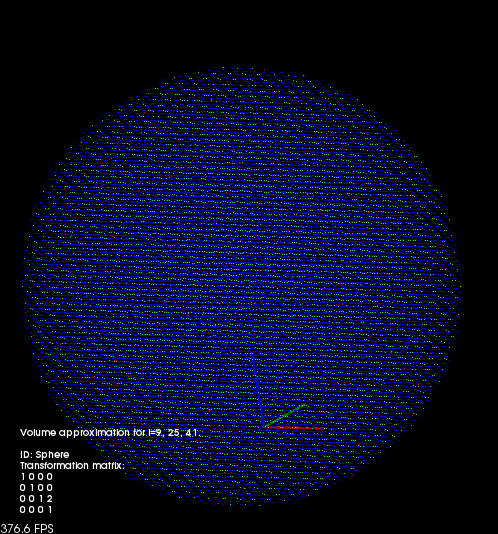
\includegraphics[width=2in]{./Results/sphere_vol}}&
    \adjustbox{valign=m}{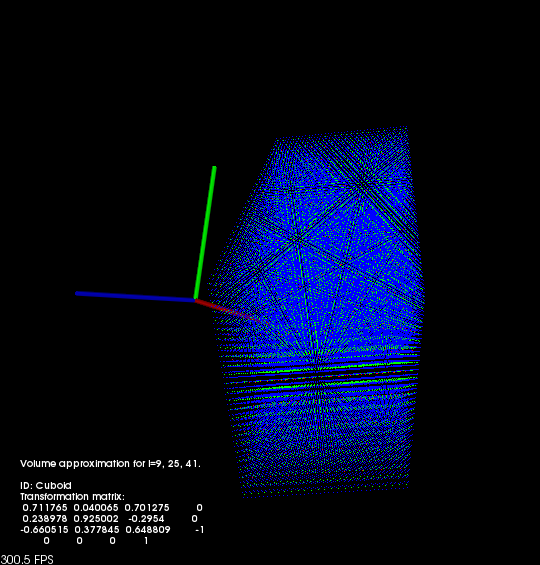
\includegraphics[width=2in]{./Results/cube_vol}}&
    \adjustbox{valign=m}{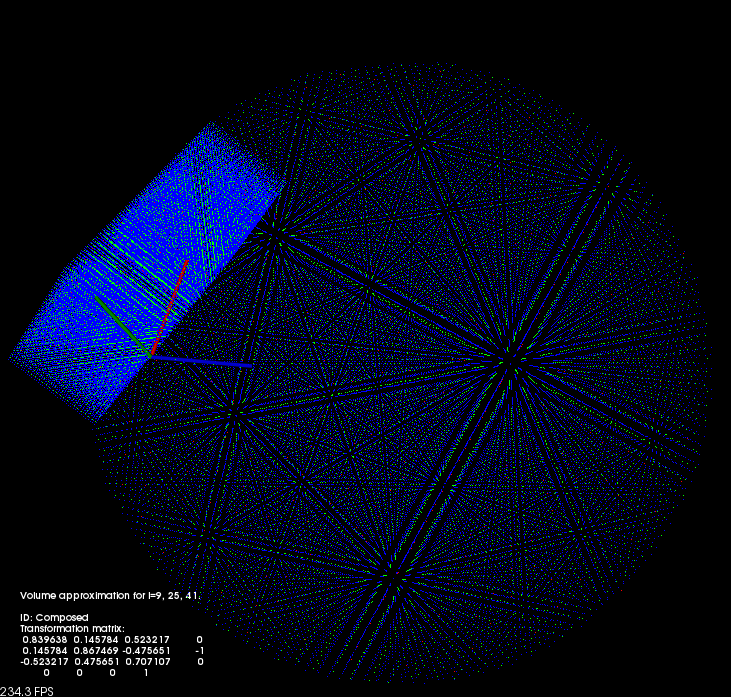
\includegraphics[width=2in]{./Results/compound_vol}} \\
    \adjustbox{valign=m}{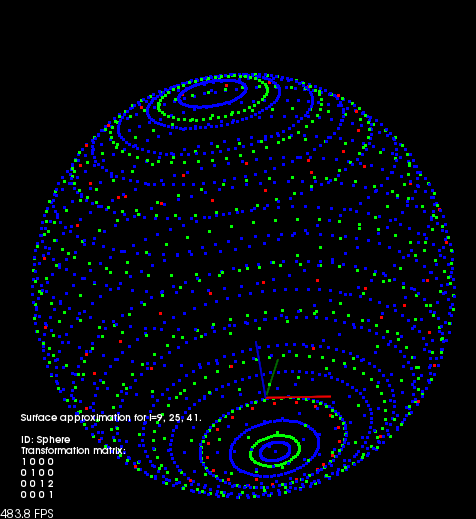
\includegraphics[width=2in]{./Results/sphere_surf}}&
    \adjustbox{valign=m}{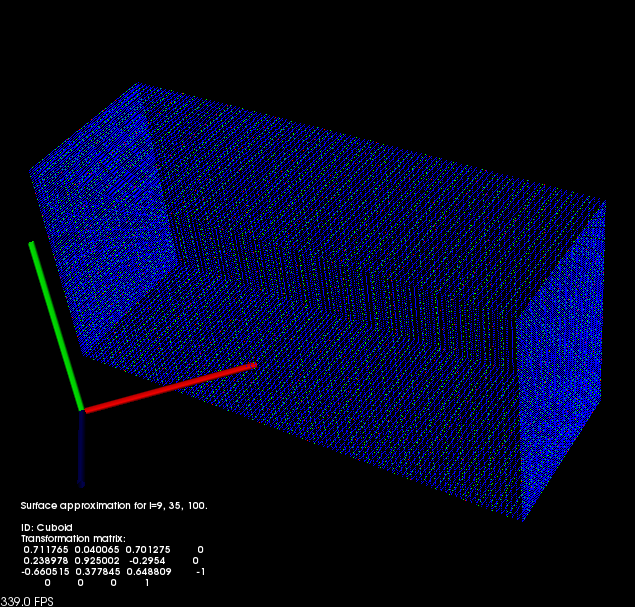
\includegraphics[width=2in]{./Results/cube_surf}}&
    \adjustbox{valign=m}{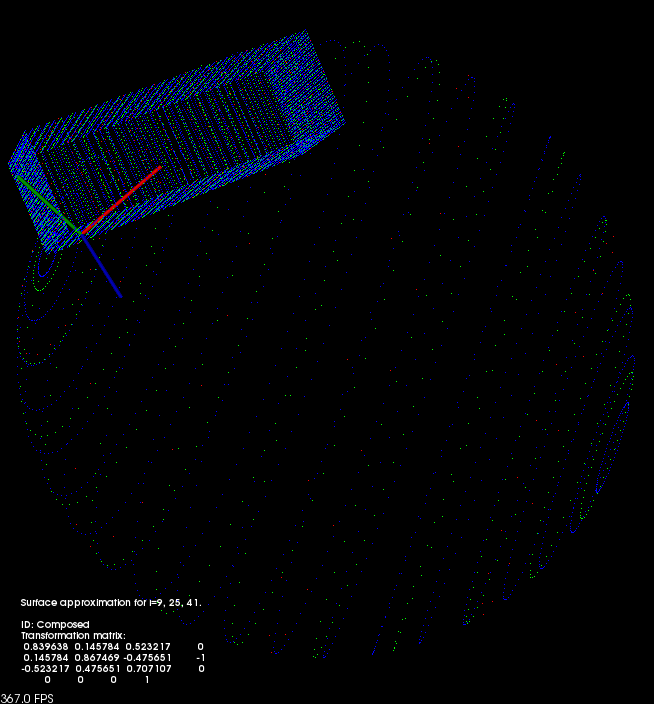
\includegraphics[width=2in]{./Results/compound_surf}}
  \end{tabular}
  \caption{Surface (top) and volume (bottom) approximation of a cube (left), a sphere (center) and a compound
  (right) for different values of $l$, depicted in red, green, and blue. \label{fig:approximate_shapes}}
\end{figure}

\subsection{Volume computation via central points} \label{volume-via-points}
After getting the approximation of the shape as a set of points, the
intersection volume is trivial to compute: as each shape knows how to check
whether a points is contained into it, it is sufficient to count the number of
points which it contain, and then assume that each point corresponds to the same
fraction of the shape's volume: $V_{\text{cube}}=\frac{V_{\text{shape}}}{N_p}$.
This assumption will be valid for sure, i.e. the computed sum will converge to
the actual intersection value if $l$ is high enough, thanks to the third
property of the approximation function stated in eqn.
\ref{eqn:points_with_constant_density}.

The total intersection volume $V_{\text{int}}$ computed with approximation level
$l$ will then be
\begin{equation}
  V_{\text{int}}(l)=V_{\text{shape}} \frac{N_{\text{in}}}{N_p(l)}
\end{equation}

\subsection{Optimized volume computations for particular cases}
The method presented in sec. \ref{volume-via-points} is universally valid,
being able to be applied for every combination of shapes. However, this is
clearly not efficient if applied to large datasets; also, the computational
complexity increases cubically with the level of approximation as stated in
eqn. \ref{volume-l-3}. Thus, when performing intersections for shapes for which
a closed form solution is known, this is preferred. In this project the case of
sphere-sphere intersection has been implemented as an example, but other cases
can be easily added due to the polimorphic structure of the algorithm.

The volume of the intersection of two spheres $S_1$ and $S_2$ can be reduced to three cases which only
depend on the distance $d$ between the centres of the spheres and their radii
$R$ and $r$, with $R\geq r$:

\begin{equation}
  V_{int}\left(S_1,S_2\right)=\left\{\begin{array}{lcr}
      0 & \mbox{if} & d\geq R+r, \\
      \frac{\pi \left(R+r-d\right) ^2 \left(
      d^2 + 2dr - 3r^2 + 2dR + 6rR-3R ^2 \right) }{12d}
      & \mbox{if} & R-r<d<R+r, \\
      \frac{4}{3}\pi r^3 & \mbox{if} & d \leq R-r.
  \end{array}\right.
\end{equation}

\subsection{Computation skipping via surface and edges intersections}
Another consideration can improve a lot the execution speed of the algorithm:
due to the real-life nature of the application scenario, the gripper will
actually seldom hit more than one object at a time. Thus, if the algorithm is
able to detect if two objects actually intersect \emph{before} computing their
volume, the resulting speedup will be important.

A sufficient and necessary condition for two shapes $S_1$ and $S_2$ to intersect is that, fixing
one of the two, at least one point of the surface $B$ of the other must be contained
into the first, or viceversa:

\begin{equation} \label{eqn:no-surface-in-volume}
  V_{\text{int}}\left(S_1,S_2\right)\neq 0 \Leftrightarrow \left(\exists P \in
    B\left(S_1\right) : P \in S_2\right) \vee \left(\exists P \in
    B\left(S_2\right) : P \in S_2\right) 
\end{equation}

When computing an intersection, the volume can thus be set to $V_{\text{int}}=0$
if no point of the surface of each shape is contained into another; as
approximating the surface of each shape results in $O(l^2)$ points, the
computation time taken by the algorithm if this strategy is applied will be
reduced by a factor $l$ if the shapes don't intersect (which is the most
probable case, given the above heuristic considerations), while the penalty for
computing the surface in case of failure of the strategy will be negligible with
respect to the volume computation's execution time.

On the other size, if of of the two shapes is fully contained into the other
one, the intersection's volume is equal to the volume of the contained shape.
A sufficient and necessary condition for a shape $S_1$ to be fully contained into
another shape $S_2$ is that all of the points of the surface $B$ of the first
are contained into the second, and none of the points of the surface of the
second are contained into the first:

\begin{equation} \label{eqn:surface-in-volume}
  S_1 \in S_2 \Leftrightarrow \left( P \in S_2 , \forall P \in B(S_1) \right)
  \wedge \left( \not \exists P \in B(S_2) : P \in S_1 \right).
\end{equation}

A lot of special cases exists for these situations too, that can improve the
execution speed (although this is asymptotically negligible, as the average
execution time will already be $O(l^3)$); for example, for cube-to-sphere
intersection, eqn. \ref{eqn:surface-in-volume} can be reduced to constant time by
noticing that it is sufficient for all the vertices $V$ of the cube to be
contained into the sphere in order for its whole surface to be contained too;
more in general, for polygonal, convex, meshes-like shapes, only the edges must
be checked to be contained one into the volume of the other. Also, if the shapes
are \emph{simply connected}, the second part of eqn. \ref{eqn:surface-in-volume}
can be omitted as it is implicitly true if the first part is. The number of
points to check is thus halved or reduced to a constant number in these cases --
which actually represent the majority of cases.



\section{Grasping poses' filtering, best grasp computation, high-level
  grasping strategy}  \label{sec:best-grasp-computation}
In this section the algorithm for selecting a set of good grasp from the set of
possible ones is presented, together with the high-level strategy for
order management, which is a closely related task for how the
implementation is done. The rationale to the  approach which is
presented here is to make the main order-management software aware of
which items can be easily grasped, and which will be difficult or
dangerous to take. In this way, by starting from the most simple ones,
it is possible for the hardest objects to take to have their way
freed and become so more accessible by the robotic arm.

When a set of poses has been generated for each object, either automatically or
manually, the main problem with it is that it will be a very big set (assuming
10 samples on each direction for each plane of the object, for example, would
lead to 600 samples for a cuboid, plus manually-added poses). As intersecting
objects is the most time-consuming task for this part, is thus
important to filter the poses in a good way.

In the project's specification it has been stated that the list of
objects to be grasped will come from a text file, and will have a
predefined bin from which the grasp will have to be done; this section
refers to this particular situation, but as it will be seen it is
trivial to make this algorithm use different constraints in order to
suite anyone's needs.

The implemented strategy goes as follows: when pose computation is required for an object,  the whole set of
its poses is put into a list and is then sorted base on preference
scores.
In this way, important poses will be tried first, and the
algorithm will be able to stop itself if a good pose has been
generated for the object which does not collide with anything into the
scene.

Taking out one by one the possible poses from this list, the main
function to compute volume intersection is called. Keeping in mind all
the heuristic strategies stated in the previous sections, the
operations described in the next paragraphs are performed.

First, an empty scene (represented as a list of shapes) is created,
located into the origin, and the shape $B$ of the bin for which the grasp has to be computed
is appended into it. This object is cached to speed up the next
computations, as each shape is able to cache its own point cloud
internally and the bin shape's approximation will probably be quite computationally
long to compute, being it a compound too.

The scene list, which is the list of objects which are present into
the bin, together with their poses, is built, and the object which has
to be taken -- identified by its index into the scene list -- is
removed. This will lead to a scene representing only objects that
the gripper will need not to bump in. This new, scene object, is then
transformed using the inverse of the object's transform: this will
make the scene make use of the object's coordinate system, in which
all the gripper's poses are.

Possible grasping poses are popped one at a time from the poses'
list. A new compound, representing the gripper into its corresponding
pose, is built now. Then the algorithm for shapes intersections is
called for each object into the scene. The score function of
sec.~\ref{grasp-score} is then computed on this result,
weighting in by means of its $\alpha$ parameter, which is used as the
already introduced movement coefficient in order to define which
objects can be bounced into without risk and which are hard or
impossible to touch; for example, the bin object will have a very high
$\alpha$ value, while lightweight objects will have $\alpha \approx
1$. At the end, a total score is computed by summing up all these
values, intersecting the gripper with the scene both into its approach and its
gripping pose.

If the total grasp score is approximately 0, i.e. below a threshold $\epsilon$, this means that the pose is
the best one, so the algorithm can stop. If the returned value is
greater than 0, a better pose could be still in the list, with a worse
preference value: in this case, the algorithm should prefer it
first. Thus, the algorithm moves on with finding another pose.

At the end of this search loop, the current best pose will be the
searched one both in terms of obstacles avoidance  and preference
score. 

\section{High-level order management} \label{sec:order-list}
With the grasping strategy described into
sec.~\ref{sec:best-grasp-computation}, it is possible to compute the
best possible grasp for each object, regardless of the current order
state, and assuming to be in an ideal situation in which the exact
pose is well-known for each object into the bin. In practice, this is
at the very least ingenuous: first, the recognition algorithm could
fail for some objects due to high occlusion or poor illumination
conditions. Second, some runtime errors (for example, the robot not
being sure whether a grasp succeded in the past) could lead a bin to a
situation in which the actual state of the bin is totally
unknown. Last, no grasping poses could have been found for an object
which guarantee no intersections at all with the rest of the scene. In
this sense, it is bad to assume that, given the best grasps for every
object, the order in which these are executed does not influence the
success of the algorithm. Given the list of objects which have to be
taken, it is thus important to \emph{sort} them in a simple way, in
order to first fulfill simplest orders, and possibly making it easier
to fullfill the most difficult ones in the subsequent iterations.

\subsection{Order list' sorting strategy} \label{sec:sort-order}
Preference score is already used when computing single grasps as a field on which ordering of
grasps is performed: however, as explained, it is preferred to be able
force a grasp to move up or down as needed. Thus, a more complete strict
ordering for grasps have been implemented:
\begin{itemize}
\item {If a grasp has been manually flagged as good, it has
  precedence over every other grasp which has been not; this is
  useful, for example, if the object is known to be the only one into
  its bin;}
\item{If a grasp has been manually flagged as bad, every other object
  which has been not has precedence over it; this can be used to mark
  objects into a bin for which the state is unknown;}
\item{The total volume of every object which has not been found into
  the bin in which the grasp has to be done is summed: grasps with a
  lower value (which is indicative of lower uncertainty over
  obstacles) have precedence over grasps with a higher one. This
  will ensure that grasps are done first if objects have been
  correctly mapped into the bins' space;}
\item{In all other cases, the normal intersection score introduced
  in \ref{sec:grasp_score} is applied.}
\end{itemize}

With this final taxel, the robot is capable of full automatic
operation. In particular, given an order list as an input, this is the
serie of steps which it will be able to do in order to complete it at
the best of its possibilities:

\begin{enumerate}
\item{At initialization time, the gripper model $G$ is read from a
  model file and stored into memory; a set of bins' position is read
  from a file too; these are treated as a set of local reference
  frames on which shapes $B_i$ will be placed when searching for a
  grasp on a specific bin, in order to consider the bins' borders; the
  bin's shapes $B_i$ are read from file too.}
\item{The input JSON file is parsed, and the contents of each bin are
  updated with the set of contained objects. When searching for a
  particular object into a bin, every object's position will be actually
  identified into it. At this time, objects' positions are all set to
  local bin origin $(0,0)$ and every bin is marked as \emph{dirty}.}
\item{A table is built to store the list of objects for which a
  valid pose has already been computed: as the poses of objects won't
  change if the robotic arm will not pass near them (i.e. in their
  bin), this will make it possible to reuse already-computed poses for
  every bin until they are actually executed or become invalid;}
\item{The order list is scanned from the JSON file, and saved in
  memory;}
\item{All depth cameras are shut down to avoid mutual interference;}
\item{For each item into the order list, if the bin corresponding to
  the object to be grasped is marked as dirty, the positions of the
  objects into its local reference system are updated. To do this, the
  camera assigned to the object is turned on, a shot is taken, and the
  camera is turned off again. After this, the precision depth camera
  is moved in front of the bin and another shot is taken, again turning on
  and off the sensor. These images are saved into a global
  bin-to-frames table. For each object which is stored into the bin,
  the corresponding recognition algorithm (mainly, Line-MOD) is
  called; the recognition process will take care of optimizing this
  process, e.g. by calling a single instance of Line-MOD for all the
  objects which can be recognized this way; after a first pass, the
  same recognition algorithm will try to refine the pose of the known
  objects using the depth image obtained previously, as explained in
  detail into the whole sec.~\ref{sec:vision}; for all the objects for which
  these algorithms converge correctly, the corresponding count of
  properly detected objects is updated into the bin status and their
  pose is saved.}
\item{Each of the objects into the order list is checked to see
  whether it has been correctly recognized at the previous step; if it
did, and its bin is marked as dirty, the best grasping pose for it is
recomputed as described in sec.~\ref{sec:best-grasp-computation}; if
this object is the only one left into its bin, this pose is marked as good;}
\item{Each dirty bin is marked as not being dirty anymore;}
\item{The order list is sorted according to the strategy of
  sec.~\ref{sort-order};}
\item{One order is popped from the top of the sorted order list, and
  the corresponding grasp is executed: first, the robotic arm moves in
  front of the bin (to have a safe starting position); then, it moves
  to the approach pose associated with the grasping pose, and finally
  to the  grasping pose itself. The gripper then returns back to the
  approach pose, and finally to the safe position;}
\item{The robot moves the object into the delivery bin and releases its grasp;}
\item{The bin from which the object has just been taken is marked as
  dirty;}
\item{If the order list is empty, the robot stops. Otherwise, the
  algorithm is restarted from point 5.}
\end{enumerate}

This is, obviously, a proof-of-concept algorithm: it does, however,
show how a robot can be programmed with extreme simplicity to
automatically grasp a complex set of heterogeneous items using the
framework developed into this project. Also, as every part of the
framework has been made with a way to expand and control it,
exploiting the strengths coming out from high-level C++ programming,
it can be seen how different strategies could be easily developed in
order to apply this same ideas with the use of different recognition
algorithms or gripping pose generations.

\section{Gripper model}
In this section the choice of the gripper mounted on the test robot is detailed
and explained. The variance within the dataset of chosen objects to grasp being
so large, the chosen gripper has been chosen in order to be as general as
possible, which is the main reason between most of the planning choices behind
it.

The gripper consists of a mounting flange to quickly mount and
dismount it on the robot's base, a aluminium shaft to let the gripper enter
easily into the objects' bin, and a serie of picking tools attached to the end
of the shaft.

The mounting flange is the one shown in fig.~\ref{fig:mounting-flange}. At one
of its side, it is adapted to fit COMAU Racer999's mounting holes. This makes
the gripper easy to mount also by nonexpert users, as mounting it only requires
screws' tightening without prior alignment. On the other side of the flange,
six mounting holes provide a solid basement for the gripper's shaft. 

\begin{figure}[htbp]
  \centering
  \includegraphics[height=3in]{./Graphics/gripper_flange}
  \caption{CAD model of the mounting flange of the gripper, depicting
  Racer999's standard mounting holes and plug for air feeding. \label{fig:mounting-flange}}
\end{figure}

The shaft is composed of a simple aluminium tube, which is both resistant enough
to hold the picking tools and picked object without damage, and slim enough to
fit the bin from which the objects will be picked. This is necessary as the
base of the robot, being it COMAU Racer999 as in this use case or another,
industrial one, will seldom be able to fit the bin with easiness, and to reach
objects close to the side of the bin itself; this would either reduce a lot the
choice of grasp possibilities, or make the grasping algorithm fail completely,
both of which are undesirable situations.

Finally, at the end of the shaft various tools can be applied. Three
tools have been attached in order for the gripper to be suitable for every
object: the preferred ones are two suckers, connected internally to an air
compressor, which can easily grasp most of the big objects, the only
requirement being their surface to be smooth enough. The two suckers are put
onto opposite sides of the shaft, and occupy almost no space on the device. Two
different sizes are needed because  the bigger one could either put too much
force on an object and damage it (using the same pressure of the smaller one),
or be too big to find a suitable surface on the object to pick, in particular
in the case of non-flat objects; the smaller sucker, in this sense, provides a
lot more options for picking poses, at the expense of worsened stability of
the grasp, especially during object's movement, due to the weaker sucking
strength. On the front side of the shaft, also, a picking plier is applied,
which is needed for the smallest or thin objects, and more in general for
every objects for which suction can't be applied: books, for example, can't be
picked properly with sucker as opening their pages could result in damage;
objects with irregular shape, also, wouldn't feel enough force because of air
losses and thus need to be picked by the closing clamp.

Both the shaft and the flange are internally cave: this lets the air and power
cables to be routed into the inner part of the gripper's body. At the middle of
the flange, this routing is exported to the external side and connections are
present for supplies.

The suckers and the plier are commanded electrically by onboard relays; these
are driven by the robot's firmware. A software has been implemented using
COMAU's proprietary language, \emph{PDL2}, as one of the main processes running on the
robot. using PDL2's APIs, the software implements a simple TCP server, which
listens for commands and toggles the gripper between five possible
configurations: in the first one (reset), the gripper just remains idle and all
the relays are shut off. This is the main state used during robot's
movement. In the three next ones (close), the gripper closes all the relays
in forward direction, making the plier close and the suckers start. The air
compression's strength can been controlled onboard for both the suckers at the
same time, by operating onto the air's closing valve. In the last state (open),
the gripper actively releases its pick, by turning on relays in reverse
direction, thus making the plier open and the suckers blow. This last state  is
necessary, especially for suckers, because if they are left idle the vacuum
created while picking the object will remain active and so the object will not
be released.

Using this gripping system, which model can be seen in fig.~\ref{fig:gripper}
every object in the set has a good number of valid grasp poses, from which the
control algorithm can choose from. Interfacing is also simple from the
programmer's side as the gripper is seen as a TCP server, and this has made it
possible to write a simple library to operate it from within every point of the
program.

\begin{figure}[htbp]
  \centering
  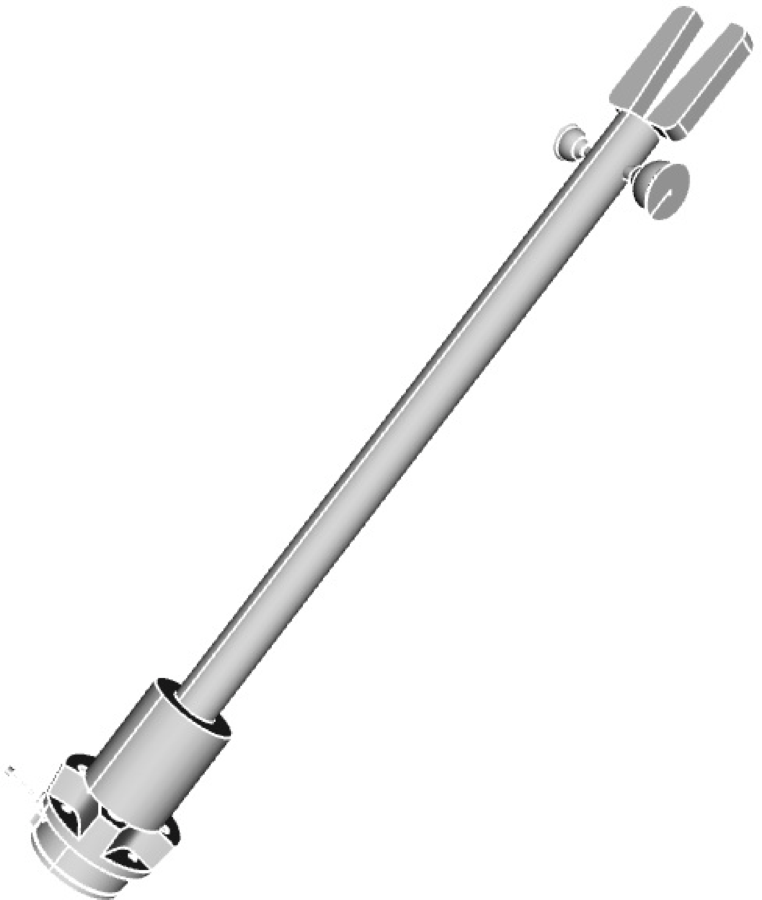
\includegraphics[height=3in]{./Graphics/gripper}
  \caption{CAD model of the gripper, with the two suckers on the sides and
  pliers on the front. \label{fig:gripper}}
\end{figure}


\subsection{Shape modelling of the chosen gripper}
After projecting the used gripper with a CAD application and producing it, the
gripper has been modelled as a shape object of the type described in sec.
\ref{sec:shapes}; naturally, it has been modeled as a compound.

After splitting the gripper into several parts, pose informations regarding
different keypoints of each part have been
extrapolated from the CAD application in order to obtain the transformation of
each compound's part with respect to its parent; this allowed to easily build
the model from scratch, and is indeed an approach that could easily be automatized by
scripting is needed.

The base flange of the gripper has been approximated to a cylinder of the same
radius and height as the flange. Cuttings into the flange have been just
ignored, which is a resonable approximation in terms of accuracy because 
of the gripper's flange being big and seldom entering the object's bin.

The gripper's main shaft can be represented with no error at all by a cylinder
of equal size.

In order to operate more comfortably onto the picking tools' representation,
all the tools have been represented together with another compound primitive,
in order to change their reference system to a system sharing the common origin
of the tools, which can be noticed from the model.

Each tool has then been represented as a single primitive, with a pessimistic
model that  
keeps into account the fact that the shapes are not convex, but concave, and if
concavities were not taken into account when computing intersections, there
would be the risk that the object could pick up something -- like a hook. Thus,
the suckers have been represented with a cylinder of radius equal to the maximum
tool's radius, while the pliers have been represented as a parallelepiped, its
dimensions being the clamps' ones when it is fully open.

When the gripper is connected to the robot, is is desiderable that the arm to
which it is attached never enters the objects' bin: it is too big to move
properly inside it and the risks of damage would be too high. Thus, another
cuboid has been added to the gripper's model, of dimensions equal to the arm's,
which will avoid this case. The rest of the arm can't be properly modeled as
the position of its shapes depend on the actual configuration of the robot's
joints, but this will never be a problem, as the lower part of the robotic arm
will never manage to reach the objects due to its limited length.

The final surface of the object's model as computed by the shape approximation
algorithm can be seen into fig. \ref{fig:approximation-of-gripper}; it does --
although without a certain margin of tolerance, especially for concavity
regions -- approximate well the gripper and is appropriate for grasping pose
computation.

\begin{figure}[htbp] \label{fig:approximation-of-gripper}
\centering
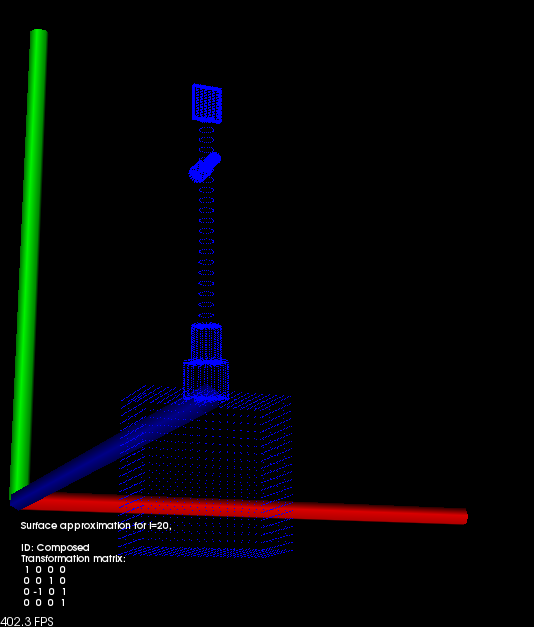
\includegraphics[height=3in]{./Results/Gripper_approx}
\caption{Gripper shape's approximation as a compound -- gripper's origin has
been moved away for visualization purposes}
\end{figure}



\section{Offline pose training}
An algorithm have been produced which can automatically generate a set of
poses, or read a set of poses from file. In this way, poses for a given object
can be generated, and heuristic poses can be given by the programmer as a hint
for the grasping algorithm.  

Each grasping pose is associated with a \emph{preference score} $P_{g}$: this will be taken
into account as a second-level sorting value for grasps, meaning that the
grasping algorithm will first search for the grasp with the lower score (i.e.
intersection volume, as described in sec. \ref{sec:grasp_score}, but in case of
a tie, it will prefer the grasp with a higher preference score.

The parameter used to assign to each grasp a preference score is the supposed
easiness to grasp the object without having it dropped during the subsequent
movement phase: for example, for the duck-toy object shown in fig.
\ref{fig:duck-toy-grasps}, a grasp done with a sucker on the plastic covering
should work properly enough, but, being the plastic covering not rigid, the
object is not sure to be taken without possibility of falling. Instead, a grasp
done with clamps on the rigid, cardboard top of the envelope would work almost
for sure. In this case, both poses would be added to the grasp list, but the
latter would be preferred if both would not make the gripper collide with the
rest of the scene.

The pose generation has been splitted into two, minor problems: indentifying a
set of points onto the object which can be used for efficient grasping, and
assigning to each point a reference frame into the gripper's model; after these
informations have been combined, the desired gripping pose is well-defined, as the
whole pose of the gripper can be computed. Problem splitting is useful in this
case, as the two parts are independent and only a little number of gripper's
reference frames -- the one corresponding to the gripper's tools -- are actually
useful for grasping. On the other hand, the problem of  generating poses for a generic
reference frame can be solved by exploiting the geometric properties of the
object itself, and this makes the algorithm agnostic with respect to the actual
gripper's shape and thus more flexible and general.

The point of connection between the two subproblems has been constrainted at the
implementation's level for simplicity's sake: all of the generated pose
points will be associated to a vector at generation time. This vector will
coincide with the tool's $Z$ axis at the time of pose binding. When describing
the pose of the tools associated with a certain set of gripping poses, it will
be sufficient to set their $Z$ axis into the operative direction (e.g. suiction
direction for suckers) in order to have the generation algorithm automatically
bind points to an actual gripper's pose.

\subsection{Pose generations on a line and on a plane's surface}
If a set of poses on a plane surface must be generated, a good method is simply
to sample the plane onto equally distanced points. Starting from the center of
the plane, which would be the preferred point for the gripper to land onto,
samples can be taken at increasing distances until the border of the surface is
reached. when doing this, it assumed that the algorithm requiring pose
generation will already have taken into account a good margin from the gripper
to operate, and so none of the poses will actually result into a gripping
failure. With this in mind, a good preference score can be obtained as the
squared distance from the gripping point $\vec{p}$ to the center $\vec{c}$ of the surface:

\begin{equation}
P_{g}=(\vec{p}-\vec{c})(\vec{p}-vec{c})^\tau
\end{equation}

Regarding the pose's orientation, the $Z$ axis is well-defined, as it will
coincide with the plane's perpendicular vector. Two cases have been considered,
as it is useful to have two different descriptions for the plane's section: if
the plane is described using a width and a height vector, named $\vec{w}$ and $\vec{h}$ the perpendicular
direction is the direction of their product:

\begin{equation}
  \vec{z_{g}}=\vec{w} \times \vec{h}
\end{equation}

On the other hand, it is helpful sometimes to describe the plane by its
perpendicular direction and center point: in this case, the $Z$ axis will just
be the same as the perpendicular vector.




\chapter{This section is just to fix TODO references, remove it after they
disappear!} \label{sec:TODO}
\printbibliography
\end{document}
